
\documentclass[subfig,blackref]{drexel-thesis}

%% Enter the appropriate information here
\author{Vincent J. Baker}
\title{Traveling waves in low-dimensional neuronal systems}
\DUTmonth{September}
\DUTyear{2021}
\degree{Doctor of Philosophy}
\advisor{Luis Cruz, Ph. D.}
\copyrighttext{\copyrighttextCCBYSA}

\usepackage[super,sort&compress,comma]{natbib} % fancy citation extensions
\bibliographystyle{unsrtnat}
%\bibliographystyle{ieeetr}
\usepackage{notoccite}

\usepackage{fancyvrb} % nicer verbatim handling
\DefineShortVerb{\|}  % \verb+TEXT+  ->  |TEXT|

\renewenvironment{preamble}{% look, we're clobbering an environment!
  What preamble?\begingroup\color{white}}{\endgroup}

\usepackage[english]{babel} % English blindtext
\usepackage{blindtext} % macros for producing dummy output
\addto\captionsenglish{\DUTnames}

%%Begin packages used in previous papers
\usepackage{amsmath}
\usepackage{times}
\usepackage{amsfonts}
\usepackage{amssymb}
\usepackage{graphicx}
\usepackage{tabularx}
\usepackage{wrapfig}
\usepackage{csquotes}
\usepackage{xcolor}
\usepackage{rotating}
\usepackage{bbm}
\usepackage{latexsym}
\usepackage{placeins}


\begin{document}
\includegraphics[width=\textwidth]{GraduateThesisSignaturePage}

\begin{DUTpreamble} % "DUT" because original preamble was clobbered.

\begin{dedications}
\rule{\textwidth}{1pt}
\\
\centering
\textsc{This thesis is dedicated to my wife Amanda and my mother Michelle.
Their unwavering support and encouragement kept me going when it would have been all too easy to abandon this work.}
\\
\rule{\textwidth}{1pt}
\end{dedications}


\begin{acknowledgments}
I would first like to thank my advisor Dr. Luis Cruz. 
His patient guidance kept me coming back to the path, despite my tendency to wander.
I'd like to thank mt commitee,  Drs. Urbanc, Richards, Liang and Rosenwinkel, for their patience with my early efforts in finding the thread of this research.
Thanks to my colleagues at Lockheed Martin's Advanced Technology Laboratories, especially the management team who allowed me to pursue my education in parallel with my professional requirements.

Finaly I would like to thank my son Alex. 
He was 9 months old when I started this journey, and I'm thrilled he got to see me finish it.
\end{acknowledgments}

\tableofcontents
\listoftables
\listoffigures

\begin{abstract}
Traveling waves of neuronal activity have been observed in many locations within the mammalian cortex.
Several functional roles have been proposed for these traveling waves including visual and audio processing, information transfer between cortical areas and memory consolidation.
Computer simulations of such traveling waves are typically performed in strictly one-dimensional or two-dimensional systems using homogeneous neurons with isotropic connectivity. 
Here we perform a computational investigation of traveling waves in more diverse systems with variations in neuron parameters and connectivity.
We explore quasi one-dimensional and quasi two-dimensional networks of heterogeneous neurons with a biologically influenced computational model of neuron dynamics and connectivity.
Our simulations reveal the model parameters for which traveling waves are supported, as well as how these parameters affect wave characteristics such as speed.
We find that a uniform random stimulus reliably evokes traveling waves in networks with local connectivity between neurons, with low-threshold-spiking inhibitory neurons influencing the wave initiation sites.
We reproduce the circular, plane and spiral wave patterns that have been observed in vivo and demonstrate the spiral waves are mroe likely to form when the inter-neuron connections are weaker.
We extend previous work suggesting that traveling waves mediate information transfer by demonstrating that traveling waves can act as an encoding and transport mechanism for neural population activity.

\end{abstract}
\end{DUTpreamble}

\begin{thesis}
\pdfbookmark[-1]{Main Matter}{Main Matter}

%%
%% This is file `example-1.tex',
%% generated with the docstrip utility.
%%
%% The original source files were:
%%
%% drexel-thesis.dtx  (with options: `example-part')
%% 
%% This is a generated file.
%% 
%% Copyright (C) 2010 W. Trevor King
%% 
%% This file may be distributed and/or modified under the conditions of
%% the LaTeX Project Public License, either version 1.3 of this license
%% or (at your option) any later version.  The latest version of this
%% license is in:
%% 
%%    http://www.latex-project.org/lppl.txt
%% 
%% and version 1.3 or later is part of all distributions of LaTeX version
%% 2003/06/01 or later.
%% 

\chapter{Introduction}
Connected neurons that fire sequentially can stimulate firings from neighboring neurons, creating a traveling wave of neuron spikes. 
These traveling waves of neuronal activation have been observed in the cortex as reviewed in \citet{Muller2018}.
Traveling waves have been observed in mammalian brains \citep{Golomb1997}\citep{reimer2010}\citep{Sato2012}  as well as in vitro \citep{wu2008}\citep{huang2004}\citep{Golomb1999}, 
and subsequently have been reproduced in silico \citep{keane2015}\citep{Senk2020}\citep{Golomb1996}\citep{ermentrout2001}. 
Various functional roles have been proposed for these traveling waves including spatiotemporal processing in the visual cortex \citep{Chemla2019}\citep{Muller2014}\citep{Nauhaus2009}, 
place field coordination in the hippocampus \citep{lubernov2009}, and memory consolidation during sleep \citep{Dickey2021}.
Traveling waves have been shown to carry information in the  motor cortex \citep{Rubino2006} and visual cortex \citep{Besserve2015}.
These waves can provide synchronous activations of a population to serve functions such as gating perception of low-contrast images \citep{Davis2020}.
In addition to extensive observations in vivo, traveling waves have also been observed in neuronal network simulations at the mesoscopic level 
in simple one-dimensional systems \citep{Wilson1973}\citep{Golomb1999} and two-dimensional sheets \citep{keane2015}\citep{Pyle2017}\citep{Townsend2018}.
Traveling waves have also been studied in large-scale simulations of the entire brain \citep{Roberts2019}.

\section{Biological observations}
Early observations of large-scale brain activity revealed oscillations in the overall neuron activity level.
Hans Berger, the pioneer of the electroencephalograph (EEG), published recorded evidence for brain waves in 1929\citep{Ince2020}.
EEG recordings revealed temporal oscillations at different frequencies that depend on the subject state.
These temporal oscillations are categorized by frequency as delta waves ($0.5-4~Hz$), theta waves ($4-8~Hz$), alpha waves ($8-12~Hz$), 
beta waves ($12-35~Hz$) and gamma waves ($\>35~Hz$).
Although EEG recordings do not have the spatial resolution required to capture the propagating behavior of traveling waves within cortical units, 
the relation between oscillation frequencies and subject state is valuable for studying traveling waves.

Techniques with higher spatial resolution are required to study traveling waves of neuronal activations.
At the microscopic level, electrodes and electrode arrays allow for measurement of electrical activity down to the individual neuron level, known as \textit{single-unit recordings}.
More often electrode arrays are used to measure the \textit{local field potential} (LFP), the average voltage in a larger volume of tissue containing multiple neurons.
Early work using local field potentials studied traveling waves in vitro\citep{Chervin1988}\citep{Golomb1997}.
These in vitro experiments involved chemical dis-inhibition and strong electrical stimulation of cortical slices to produce traveling waves.
Early work with in vivo local field potentials found temporal oscillations \citep{sanes1993}.
\citet{Rubino2006} measured propagating waves in the motor cortex of monkeys using local field potentials 
and similar waves have been observed in local field potentials in human subjects\citep{Takahashi2011}.
\citet{Riehle2013} combined simultaneous recordings of both local field potentials and single-unit recordings from the motor cortex.

Mesoscopic traveling waves have also been observed with optical imaging techniques using \textit{voltage-sensitive dyes} (VSD).
These techniques measure neuronal activity with simultaneous high spatial and temporal resolution \citep{Grinvald2004}\citep{Shoham1999}. 
\citet{wu2008} provides a review of the use of VSD techniques to image traveling waves.
VSD imaging has revealed complex spiral patterns in vitro \citep{huang2004} and wave compression and refraction in vivo\citep{Xu2007}.
Since VSD can be used to record cortical dynamics from awake and freely moving subjects \citep{Muller2014}\citep{Ferezou2006}, 
VSD creates a powerful tool to study reasoning primates.  

Further advances in both electrode arrays and data processing techniques have provided competitive results to 
VSD when measuring traveling waves from LFPs and single-unit recordings.
\citet{Besserve2015} analyzed LFP using \textit{transfer entropy}, an information-theoretic technique for determining directed information flow,
to show that a visual stimulus could change the direction of gamma-band waves in the visual cortex
\citet{Takahashi2015} used a similar information-theoretic technique known as \textit{Granger causality} with a combination of LFPs and single-unit recordings
to demonstrate that the waves detected using LFPs in the motor cortex are also detectable using the single-unit recordings.
Further advances in both electrode arrays\citep{Maynard1997} and data processing techniques\citep{Muller2016} have allowed researchers to detect traveling waves in electrode data 
related to visual processing\citep{Davis2020} and memory consolidation\citep{Dickey2021}.

Traveling waves have been extensively studied in the primate brain, and new experimental and data processing techniques 
continue to expand our understanding of spatiotemporal dynamics in the cortex.
To fully understand the functional role of traveling waves will require corresponding higher fidelity simulations of cortical dynamics.

\section{Large-scale approximate models}
Traveling waves have been studied in high-level approximate models of neuronal systems.
Two of the most relevant approaches have used mean-field approximations and coupled oscillators as behavioral representations of large collections of neurons.
These approaches provide computational tractability and insight into large-scale behaviors but can not fully capture the complex behavior of coupled systems with the wide variety of neuronal, 
synaptic and dendritic dynamics found in the brain.

Mean-field models attempt to reduce the complex activity within a large population of neurons to a set of mean-field equations.
One of the earliest uses of a mean-field approaches was developed by Amari\citep{Amari1972}\citep{Amari1977}.
Wilson and Cowan\citep{Wilson1973} created one of the earliest models that showed traveling waves. 
They developed equations for neuronal activity as a function of position and time in a one-dimensional system and showed that there exist traveling waves solutions of those equations.
This approach was further expanded \citep{Ermentrout1979}\citep{Sompolinsky1988}\citep{Vreeswijk1998}\citep{Faugeras2009}\citep{Zhang2016} to neural field models incorporating 
varying degrees of heterogeneity in the neuron dynamics and connectivity models.
Traveling waves emerge as solutions of most of these mean field equations.
This is not surprising since the topology and connectivity of the underlying neurons are assumed to be regular and isotropic, naturally leading to 
spatially periodic potentials with traveling wave solutions similar to crystal lattices in solid-state physics.

Large systems of neurons have also been studied using coupled oscillator models.
Kopell and Ermentrout \citep{Kopell1986} considered chains of weakly coupled oscillators with symmetric coupling and found stable wave solutions of their equations.
The coupled oscillator model is also applied to pulse-coupled oscillators \citep{Ermentrout1990}\citep{Mirollo1990}. 
Ermentrout and Kleinfeld \citep{ermentrout2001} separated wave-like behavior into three categories: delayed excitations from a single oscillator, 
propagating pulses in an excitable network and phase-locked weakly coupled oscillators.
We consider the traveling waves observed in our work to belong to the first two classes.

These approximate models have provided useful characterization of the average dynamics of cortical regions.
They provided a computationally tractable method for predicting behavior of systems composed of many neurons.
However, these models obscure many of the real variation and anisotropy in the dynamics of systems of real neurons, axons, synapses and dendrites. 

\section{Spiking neuron models}
Neurons are complex biological assemblies, and neuron membrane potentials are driven by electrochemical processes.
When the internal neuron dynamics are disturbed far enough from equilibrium there is a sudden depolarization of the membrane potential, followed by an equally sudden return to the equilibrium state.
This disturbance, termed a neuron spike, results in an electrochemical signal that is sent down the neuron's axis and transmitted to many other neurons through synaptic connections 
to the post-synaptic neuron's dendrites.
The axons, synapses and dendrites all have their own rich electrochemical dynamics that determine the post-synaptic neurons response to the spike.
We review computational models of the neuronal system that are relevant to traveling waves of neuronal activations.

Biophysical modeling of the neuronal systems largely began with Hodgkin and Huxley's work on the giant squid axon \citep{Hodgkin1952}.
Their equivalent electrical model included three ionic currents and the resulting set of four differential equations is still used in neuron modeling today.
The Hodgkin-Huxley type of model has been further extended to include more ion channels\citep{Wilson1999}, resulting in more complex models that can better replicate spiking patterns observed in biological neurons.
Large simulation frameworks such as NEURON allow researchers to simulate neural systems with high fidelity models of neurons, axons, synapses and dendrites.
These types of models capture the underlying electrochemical processes but are computationally expensive, 
so simpler models must be used when modeling structures of many neurons across long time intervals.

Simplified models of the neuron have been developed to represent the fundamental neural processes in a mode feasible for simulating systems of many neurons.
McCulloch and Pitts\citep{McCulloch1943} developed one of the earliest simplified models of a neuron:
\begin{align}
  \begin{split}
    g(x_1,x_2...x_n) &= g(\boldmath{x})=\sum_{i=1}^n x_i \\
    y = f(g(x)) &= 1 \text{ if } g(x)>\Theta \\
		&= 0 \text{ if } g(x)<\Theta \\
  \end{split}
\end{align}
The \textit{McCulloch-Pitts} model includes several features used in many computational models.
It sums the values from many input neurons \textbf{x}, applies an \textit{activation function} f, and provides an all-or-nothing response based on a threshold $\Theta$.

Many phenomenological studies use the \textit{leaky integrate-and-fire} (LIF) model\citep{Abbott1999}. which may be stated as in (\citet{Trappenberg2010} Section 3.1.1):
\begin{align}
  \begin{split}
    \tau_m \frac{dv(t)}{dt} &= -(v(t)-E_L) + RI(t) \\
    \displaystyle\lim_{\delta \rightarrow 0} v(t^f + \delta) &= v_{res}\\ 
    I(t) &= \sum_j \sum_{t^f_j}w_j\alpha(t-t^f_j)
  \end{split}
\end{align}
where $v(t)$ is the membrane voltage of a neuron, $\tau_m$ is the membrane voltage time constant, $E_L$ is the equilibrium membrane voltage, $R$ is the membrane resistance, and
$I$ is the current due to the sum of spikes from presynaptic neurons $j$ at times $t^f_j$ transformed by a synapse response function $\alpha$ and weighted by synaptic conductances $w_j$.
The second line is a reset that is performed when the membrane voltage reaches the spike threshold and fires a spike at time $t^f$.
The LIF model captures the all-or-nothing spiking behavior of biological neurons as well as the tendency of a neuron that is slightly perturbed from equilibrium to return to equilibrium,
The synaptic weights in the LIF model can capture the stochastic connectivity of biological neurons, and the model can represent excitatory and inhibitory presynaptic neurons through the signs of the $w_j$.

There is a third class of neuron models that seeks to represent the dynamics of neurons without explicitly calculating the ionic currents.
These models use principles of dynamical systems in phase space such as equilibrium, limit cycles and bifurcation to represent neuron dynamics with simplified models.
For our work we choose the Izhikevich model\citep{izhikevich2003} which is fully described in Methods.
The Izhikevich model can replicate neuron behaviors not captured in the LIF model including variable spiking rates, intrinsic bursting, chattering, post-inhibitory rebound spiking and low-threshold spiking.
The original presentation of the model also includes stochastic parameter values to represent the variation in dynamics seen in cortical neurons.

\section{Traveling waves in spiking neuron models}
Traveling waves have previously been shown in simulations of neurons.
One-dimensional waves have been observed in simulations using firing rate neurons \citep{Roxin2005}, integrate-and-fire neurons \citep{Bressloff1997}\citep{Golomb1999} and Hodgkin-Huxley neurons \citep{Golomb1997}.
\citet{Senk2020} used populations of both rate neurons and integrate-and-fire neurons and developed a method to translate parameters between the two different models.
More recently, two-dimensional waves of multiple types have been studied using integrate-and-fire neurons \citep{Mehring2003}\citep{keane2015}\citep{Keane2018}\citep{Spreizer2019}\citep{Chen2019}.
It is somewhat surprising that a  more complete study of traveling waves in simulation has not been undertaken given the extensive biological observations of traveling waves
and their proposed functional significance.

\section{Neuromorphic processing}
Although our primary interest lies in understanding cortical function there are also applications of our modeling to purely computational systems.
Modern machine learning is focused on feedforward networks with the equivalent of McCulloch-Pitts neurons.
Recurrent networks of spiking neurons may offer a more powerful, energy-efficient computational paradigm.
Modern work on analog neural networks including photonic neurons\citep{Xiang2016}\citep{Coarer2018}\citep{Fok2010} and electrical neurons has shown the potential for low power computation.

Traveling waves in analog systems have been proposed as an efficient machine learning platform\citep{Hughes2019}.
Advanced electronic and photonic systems are largely two-dimensional based on the methods required to create dense integrated circuits.
Two-dimensional systems of spiking neurons are likely to favor local connectivity as it is difficult to route many long-range connections in a two dimensional geometry.
A spiking neural processor with local connectivity would be expected to exhibit traveling waves.
Therefore, understanding the mechanisms and functional roles of two-dimensional traveling waves may provide insights into analog neural processors.

\section{Thesis Organization}
The remainder of the thesis includes a chapter on the methods used, three chapters presenting the research and results, and a conclusion.

We first discussed the common Methods used in this research in Chapter 2.
We describe the models used for neuron dynamics and neuron connectivity.
We also describe our methods for characterizing neuronal systems and for detecting traveling waves.

Chapter 3 covers quasi one-dimensional systems. 
We introduce our model of a neuronal minicolumn and present the relevant model properties.
We present reference model parameters  that are used throughout the work.
We show that traveling waves are supported in these minicolumn structures and vary the model parameters about the reference point 
to characterize the effect of the model parameters upon traveling wave formation.
We find that \textit{low-threshold-spiking} (LTS) inhibitory neurons can act as wave generators in our system.
We also identify spatiotemporal patterns that look like traveling waves but arise from axonal conduction delay instead of local connectivity.

Chapter 4 covers two different types of two-dimensional systems.
We first examine traveling waves in a 2-D sheet of neurons.
We find several types of 2-D waves including circular spreading waves and plane waves.
We also find that rotating spiral waves emerge with weaker connectivity between the neurons.
We again find that LTS inhibitory neurons acting as wave generators.
The second 2-D model is a forest of minicolumns where the lateral extents of the forest are much longer than the length of the individual minicolumns.
The separation between minicolumns is greater than the separation between the neurons within the minicolumns,
resulting in an anisotropic connectivity.
We see waves spreading laterally through the forest, but the lateral waves propagate more slowly than the vertical waves down the minicolumns.

Chapter 5 explores a functional role of traveling waves as carriers of information.
We show that our minicolumns can encode and transmit the average firing rate of a population of neurons.
The population rate is encoded into the traveling wave rate within the minicolumn.
The graph of traveling wave rate against population firing rate resembles the activation functions of individual neurons or 
populations of neurons when exposed to a constant stimulus.
We therefore term this relation the \textit{activation function} of the minicolumn.
The population activity encoding via a single minicolumn is noisy and unreliable,
but we find that our forest of minicolumns has a reliable activation function with low variance.

Chapter 6 provides a conclusion, summarizing this work and suggesting future research.


\endinput
%%
%% End of file `example-1.tex'.

%%
%% This is file `example-1.tex',
%% generated with the docstrip utility.
%%
%% The original source files were:
%%
%% drexel-thesis.dtx  (with options: `example-part')
%% 
%% This is a generated file.
%% 
%% Copyright (C) 2010 W. Trevor King
%% 
%% This file may be distributed and/or modified under the conditions of
%% the LaTeX Project Public License, either version 1.3 of this license
%% or (at your option) any later version.  The latest version of this
%% license is in:
%% 
%%    http://www.latex-project.org/lppl.txt
%% 
%% and version 1.3 or later is part of all distributions of LaTeX version
%% 2003/06/01 or later.
%% 

\chapter{Methods}
To study traveling waves in small columnar ensembles (SCE) of neurons we created a MATLAB simulation of our model based on \citet{izhikevich2003} . 
We first construct these assemblies by placing neurons at the vertices of a cubic lattice described by two short  dimensions (X,Y) and one long dimension (Z). 
Each neuron is  randomly chosen to be  either excitatory (E) or inhibitory (I), with the fraction of excitatory neurons indicated as $P_{exc}$.
After placing, we connect two neurons based on their relative distance according to a connection probability that favors local connectivity given by  \citep{maass2002}: 
\begin{align}\label{eq:connectivity}
 P_{a,b} &= C e^{-(D(a,b)/\lambda)^2}
\end{align}
where $D(a,b)$ is the Euclidean distance between neuron A and B, $\lambda$ is the characteristic length of the local connectivity neighborhood, and $C$ is the peak probability of connection .
In \citep{Levy2012} the authors showed that the synaptic connections in the mouse auditory cortex follow this connection probability.
Multiple connections from the same presynaptic neuron to the same postsynaptic neuron, as well as self-connections, are prohibited.
Two neurons may be recurrently connected, however. 
We use open boundary conditions, so neurons near the ends of the SCE will have fewer connections than those in the middle.
An example of an SCE showing the connectivity structure is shown in Figure \ref{fig:column_structure}.
\begin{figure}[!htb]
 \caption{Example SCE with dimensions 2x2x10 (XxYxZ), $\lambda$=2.5, and C=1. A)  SCE showing connections between neurons as lines colored using a color scale that indicates the connection length. 
 B)  Connection matrix. E-E connections are green, E-I are black and both I-E and I-I  are red. 
 The labels of the neurons used in both axes are sequentially assigned starting at the bottom (Z=0).
 C) The sum of presynaptic weights for each neuron shows the anisotropy of this model, with substantial variation in input strength and sign between the neuron inputs.}
 \label{fig:column_structure}
 \subfloat[][]{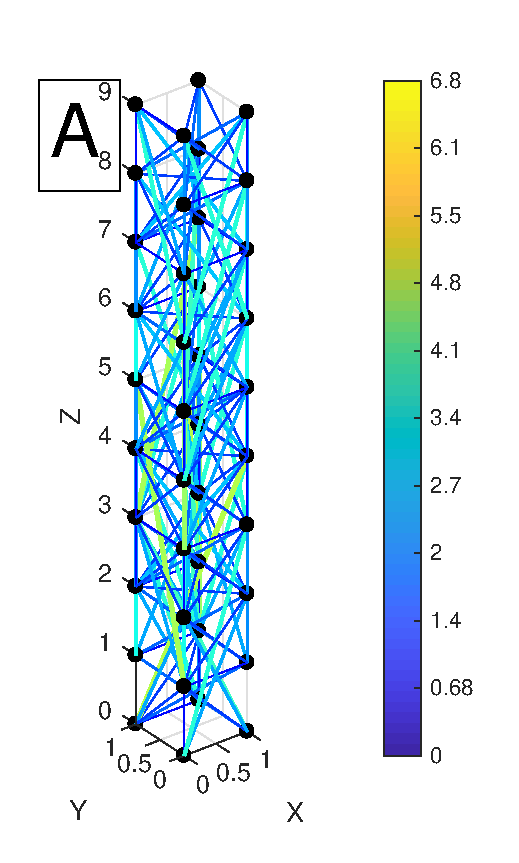
\includegraphics[height=60mm]{fig/column_structure_A}}
 \subfloat[][]{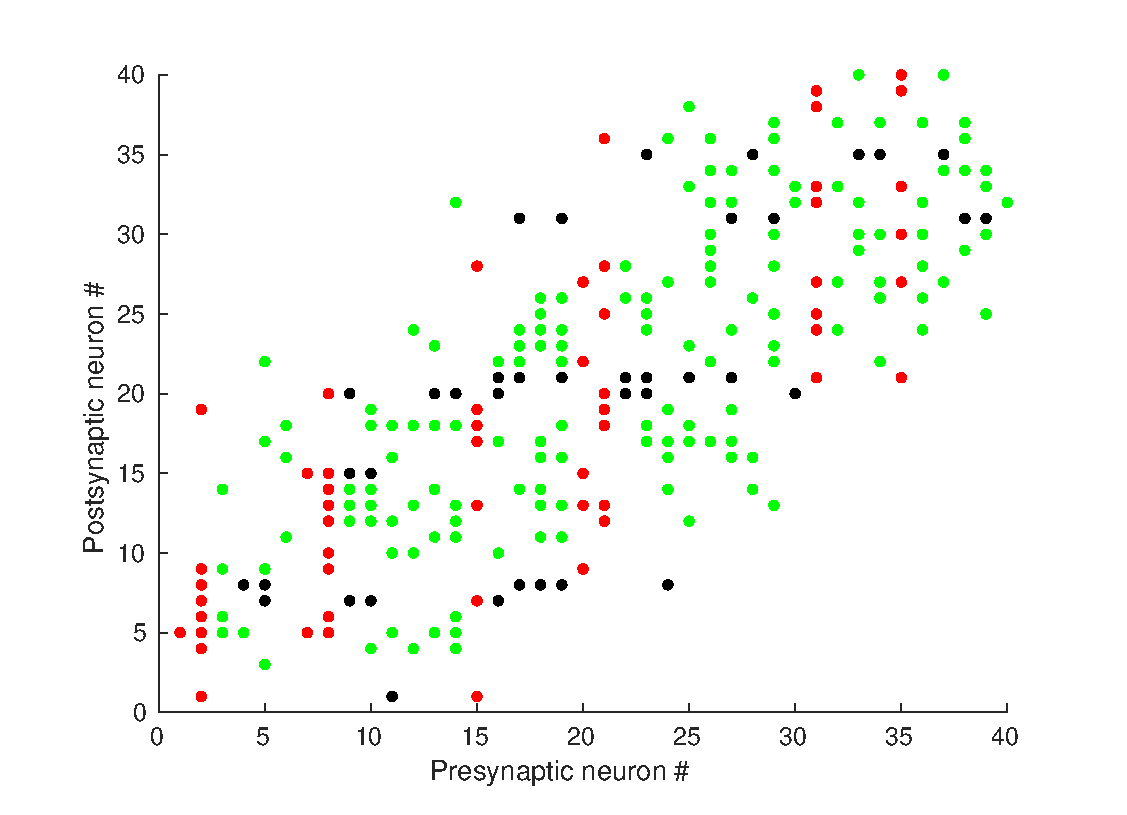
\includegraphics[height=60mm]{fig/column_structure_B}}
 \subfloat[][]{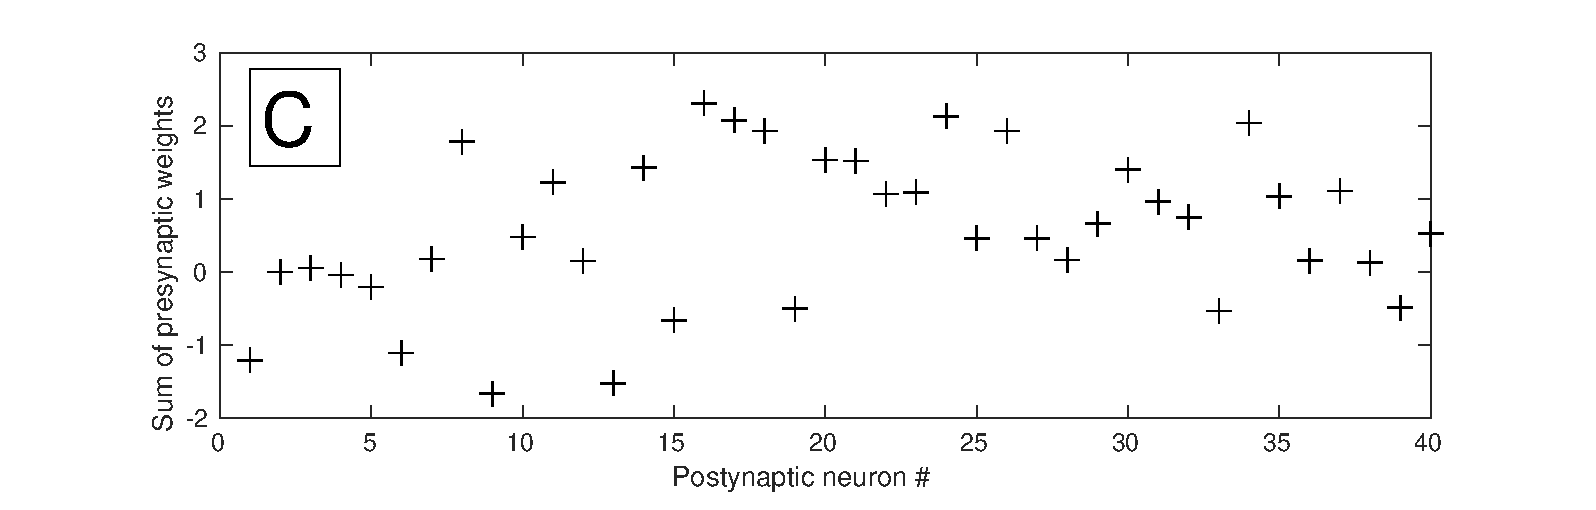
\includegraphics[width=\textwidth]{fig/column_structure_C}}
\end{figure}

A crucial element in neuronal systems is the existence of time delays between the creation of a presynaptic action potential and the arrival of that spike to a target neuron. 
We use distance-dependent time delays for the propagation of a spike from neuron $i$ to neuron $j$ of $\tau_{ij} = \kappa  D(i,j)$. 
The constant of proportionality $\kappa$ ranges from $0$ to $4$.
When $\kappa=0$ the action potential excites the post-synaptic neuron on the succeeding simulation time step.
 
The distribution of post-synaptic connections and delay times are shown in Figure \ref{fig:connection_delay_distrbution} for an example minicolumn.
\begin{figure}[!htb]
 \caption{Distribution of (A) number of post-synaptic connections per neuron and (B) delay time. Data was taken over 100 realizations of a 2x2x50 SCE, $\lambda=2.5$, $\kappa=1$.  } 
 \begin{tabular}{c}
     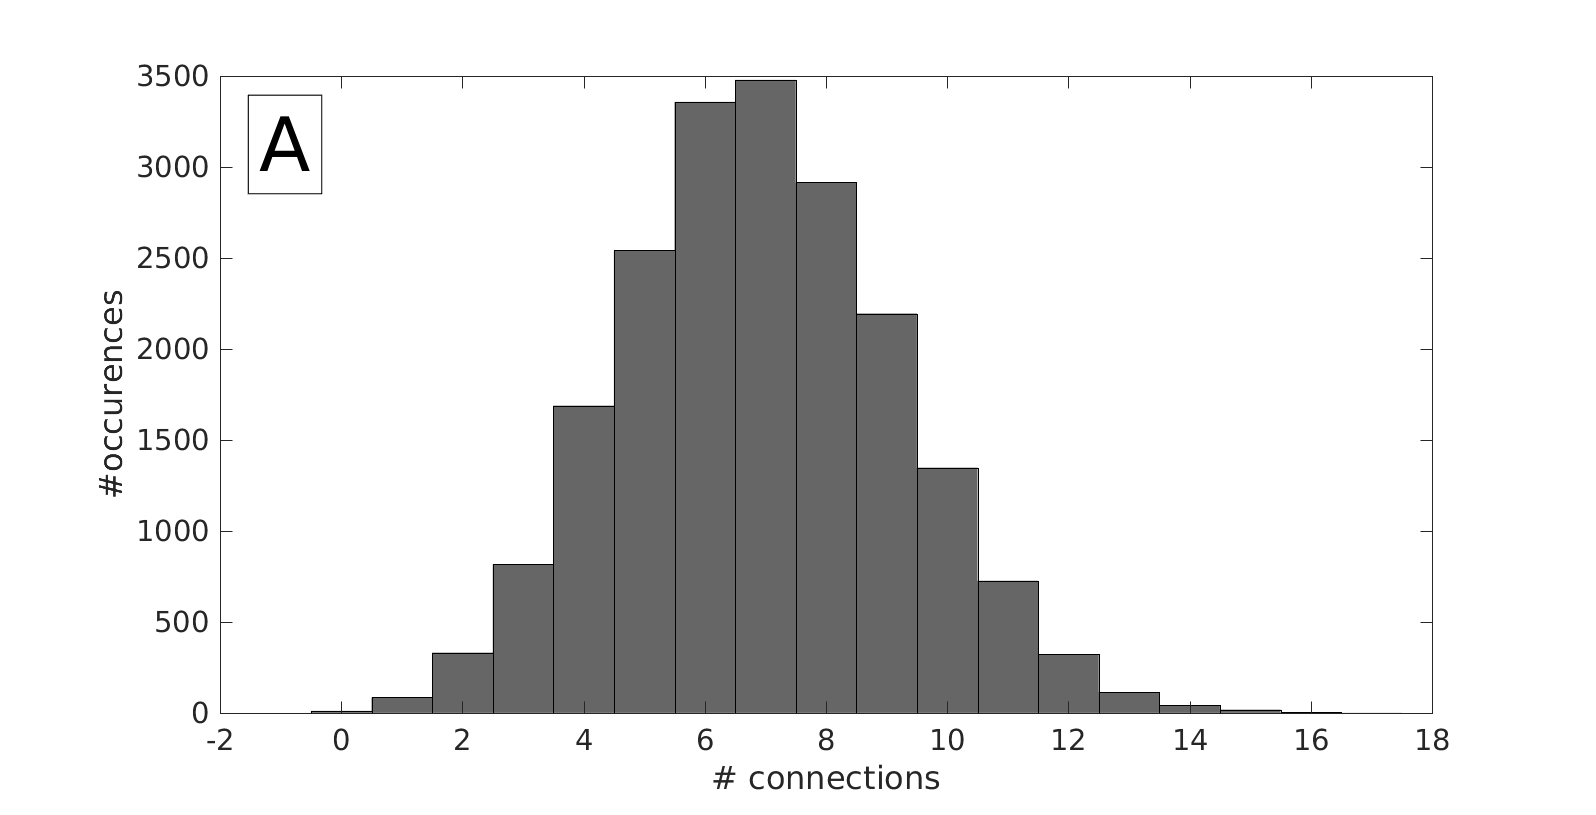
\includegraphics[width=\textwidth]{fig/ConnectionNumberDistribution} \\
     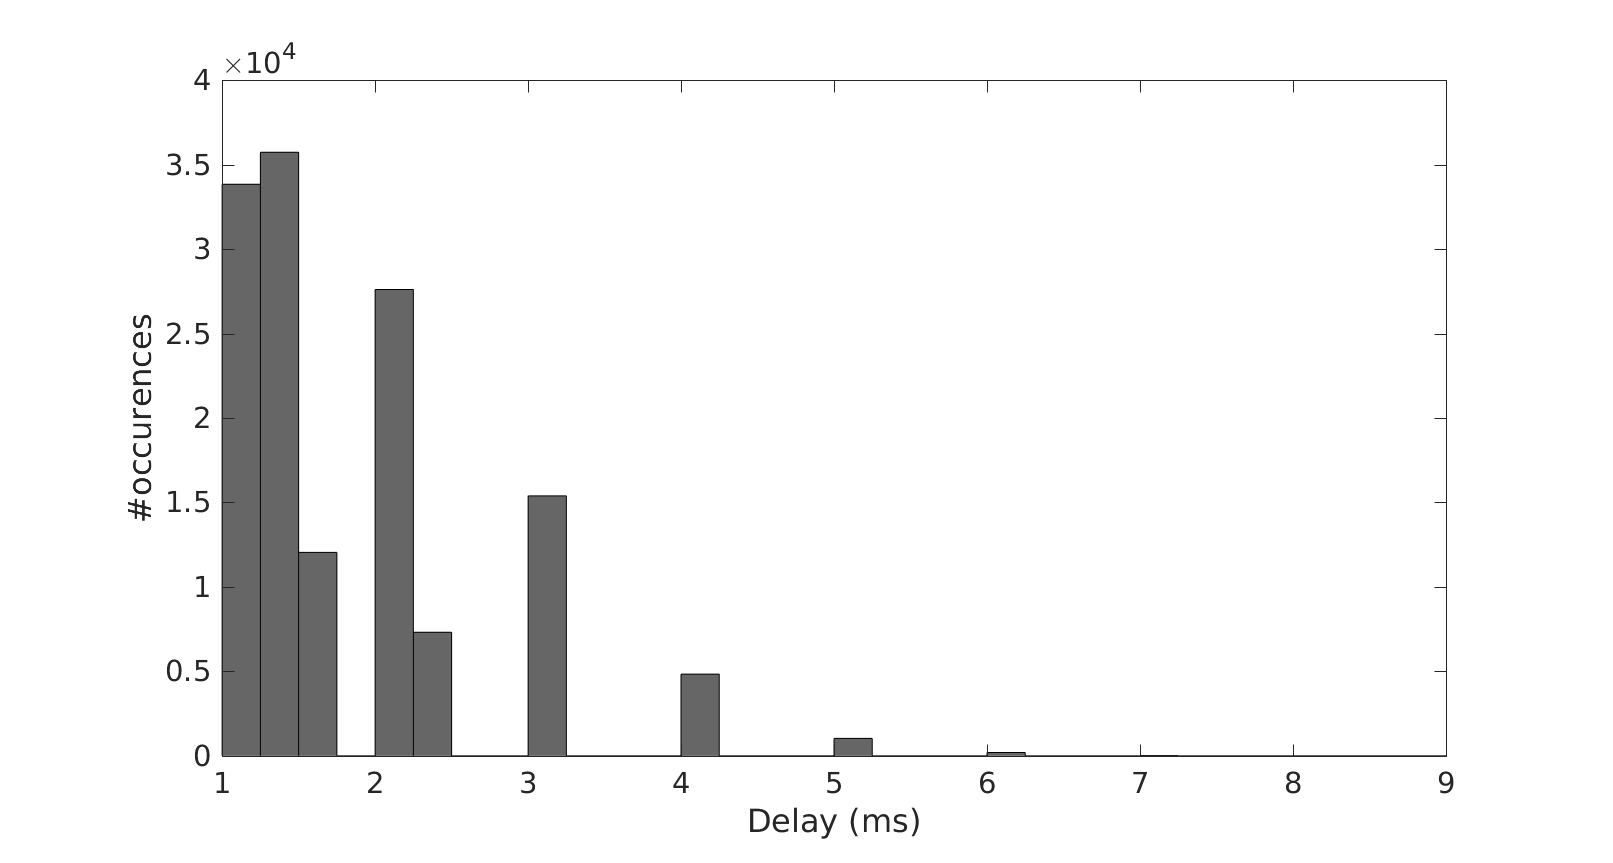
\includegraphics[width=\textwidth]{fig/DelayDistribution} 
 \end{tabular}
 \label{fig:connection_delay_distrbution}
\end{figure}
 \FloatBarrier

We model the firing dynamics of each neuron using the Izhikevich model \citep{izhikevich2003} that consists of a two-dimensional model of two coupled differential equations given by:
\begin{align}
 \begin{split}
  v^\prime &= 0.04v^2+5v+140-u+I \label{eq:neuron_v} \\
  u^\prime &= a(bv-u)
 \end{split}
\end{align}
where $v$ is the membrane potential of the neuron and $u$ is a membrane recovery variable, with a spike threshold and an auxilliary after-spike resetting of parameters by:
\begin{align}
  \text{if } &v>30: v\leftarrow c, u\leftarrow u+d
\end{align}
and I is the sum of all incoming currents to the neuron, explained in detail below. 

Equation \ref{eq:neuron_v} has four parameters (a,b,c,d) that with specific values can model a wide range of neuronal spiking behavior \citep{izhikevich2003}. 
The parameters used here (see Table \ref{tab:izzy_params}) are based on those specified in \citep{izhikevich2003} with modification of the $c$ parameter for excitatory neurons and define a random population of neurons where $U(s,t)$ represent a number drawn from a uniform random distribution between s and t. 
\begin{table}[!htb]
 \caption{Izhikevich model parameters}
 \label{tab:izzy_params}
 \centering
 \begin{tabular}{lcr}
  \textbf{Parameter} & \textbf{Excitatory} & \textbf{Inhibitory} \\
  \hline
  a & 0.02 & 0.02+$\mathcal{U}$(0,0.08) \\
  b & 0.2 & 0.25-$\mathcal{U}(0,0.05)$\\
  c & -65+$\mathcal{U}(0,10)^2$ & -65 \\
  d & 8-$\mathcal{U}(0,6)$& 2 \\
 \end{tabular}
\end{table}
For solving equation (2) numerically we use the modified Euler method from \citep{izhikevich2003} with a time step of $0.2 ms$ except were noted. 


The current I in equation (2) includes the sum of all incoming stimuli into neuron $i$ from other neurons $I_i$ and external stimuli $I_{i,e}$ applied to the system. 
The neuron-neuron incoming current $I_i$ into neuron $i$ is given by:
\begin{align}
 I_i(t) &= \sum_{j\ne i} \sum_{t^\prime_j} S_{ij}  \Theta(t-t^\prime_j-\tau_{ij})e^{-(\frac{t-t^\prime_j-\tau_{ij}}{\sigma_s})^2}
\end{align}

where $t'_j$ are the firing times of neuron $j$, $\Theta$ is the Heaviside step function, and the exponential factor models an exponentially decaying synapse response with a time constant of $\sigma_s = 4 ms$. 
The $S_{ij}$ represent the connection strengths between presynaptic neuron $j$ and postsynaptic neuron $i$ given by
\begin{align}
 \begin{split}
  S_{ij}^{excitatory} &= K \times \mathcal{U}\{0,0.5 \} \\
  S_{ij}^{inhibitory} &= K \times \mathcal{U}\{-1,0 \} 
 \end{split}
\end{align}

where $K$ is a parameter that modulates the strength of connections, with $K=1$ corresponding to the original model in \citep{izhikevich2003}. 

To drive the firing dynamics and create traveling waves we provide stimulation to the systems by using two different and separate external stimulus currents, $I_{i,e}$. 
One of them is a uniform background stimulus applied to each neuron $k$ that depends on whether the neuron is excitatory or inhibitory.
The stimulus values are drawn from a random distribution every $1 ms$ according to:
\begin{align}\label{eq:randomstim}
 \begin{split}
  I_k^{excitatory} &= M \times \mathcal{U}\{0,1 \} \\
  I_k^{inhibitory} &= \frac{2}{5} M \times \mathcal{U}\{0,1 \}
 \end{split}
\end{align}
where $M$ is a parameter that tunes the overall strength of the stimulus, with $M=5$ corresponding to the original model in \citep{izhikevich2003}. 
This stimulus has the effect of creating waves that originate from any point along an SCE and one of the uses is to study interactions between multiple waves in section \ref{sub:wave_initiation}.

The other external stimulus $I_{i,e}$ is a short constant input of current applied to all of the neurons in the lowest ten layers of an SCE. 
The duration of the stimulus is $20 ms$ with a current of strength $5$ units. 
This stimulus has the effect of creating a single wave that can propagate through the total length of an SCE.
One of the uses of this stimulus is to measure the speed of the traveling wave in section \ref{sub:propagation_speed}.

We summarize our model parameters in Table \ref{tab:all_params}. 
\begin{table}[!htb]
 \caption{Model Summary}
 \label{tab:all_params}
 \centering
 \begin{tabular}{c}
  \textbf{Model} \\
  \hline \\
 \end{tabular} \\
 \begin{tabular}{ll}
  Population & Excitatory, inhibitory \\
  Topology & Small columnar ensemble, Z extents $\gg$ X,Y extents \\
  Connectivity & Stochastic, $P_c$ exponentially decays with distance between neurons \\
  Neuron model & Izhikevich model with distribution of neuron parameters \\
  Synapse response & Exponential synaptic response with randomized peak connection strength  \\
  Spike propagation & Delay proportional to distance, Fixed propagation time \\
  Input & Random input to all neurons, Fixed stimulus to neurons at the bottom of the SCE \\
 \end{tabular}
\end{table}

For every simulation we record all of the spikes from all neurons. 
We visualize the spikes in spike raster plots (e.g. Figure \ref{fig:sigma_raster} ).
Because here we focus on traveling waves in the Z direction, we plot the spikes according to the Z position of the neurons.
As a consequence, at each Z position there are multiple neurons that could contribute to the spike raster plot at that Z coordinate (e.g. 4 neurons for the X=2, Y=2 SCE case).

To automatically identify waves we perform a spatial clustering operation to this data to identify spatiotemporal regions identified by high firing density. 
The clustering operation produces an output cluster for any group of more than $3$ spike events that fall within a $20ms$ time window from neurons that are no more than $3$ layers apart.
Each cluster $C(t,z)$ has a time $t$ and position $z$.
This clustering removes random background firing activity. 
The waves are identified using a plane sweep algorithm that proceeds along the dimension of simulation time and applies wave labels to clusters such that all clusters with the same label are part of the same wave.
When a new cluster $C(t,z)$ is encountered, the algorithm associates $C(t,z)$ with any existing wave if the existing wave has a cluster $C(t_c,z_c)$ within $40 ms$ and $6$ units of the new cluster.
If there is no such adjacent cluster a new wave is created using $C(t,z)$ as the first cluster.

An example of the clustering and identification is shown in Figure 2, with further illustration in SI Figure 1.
\begin{figure}[!htb]
 \centering
 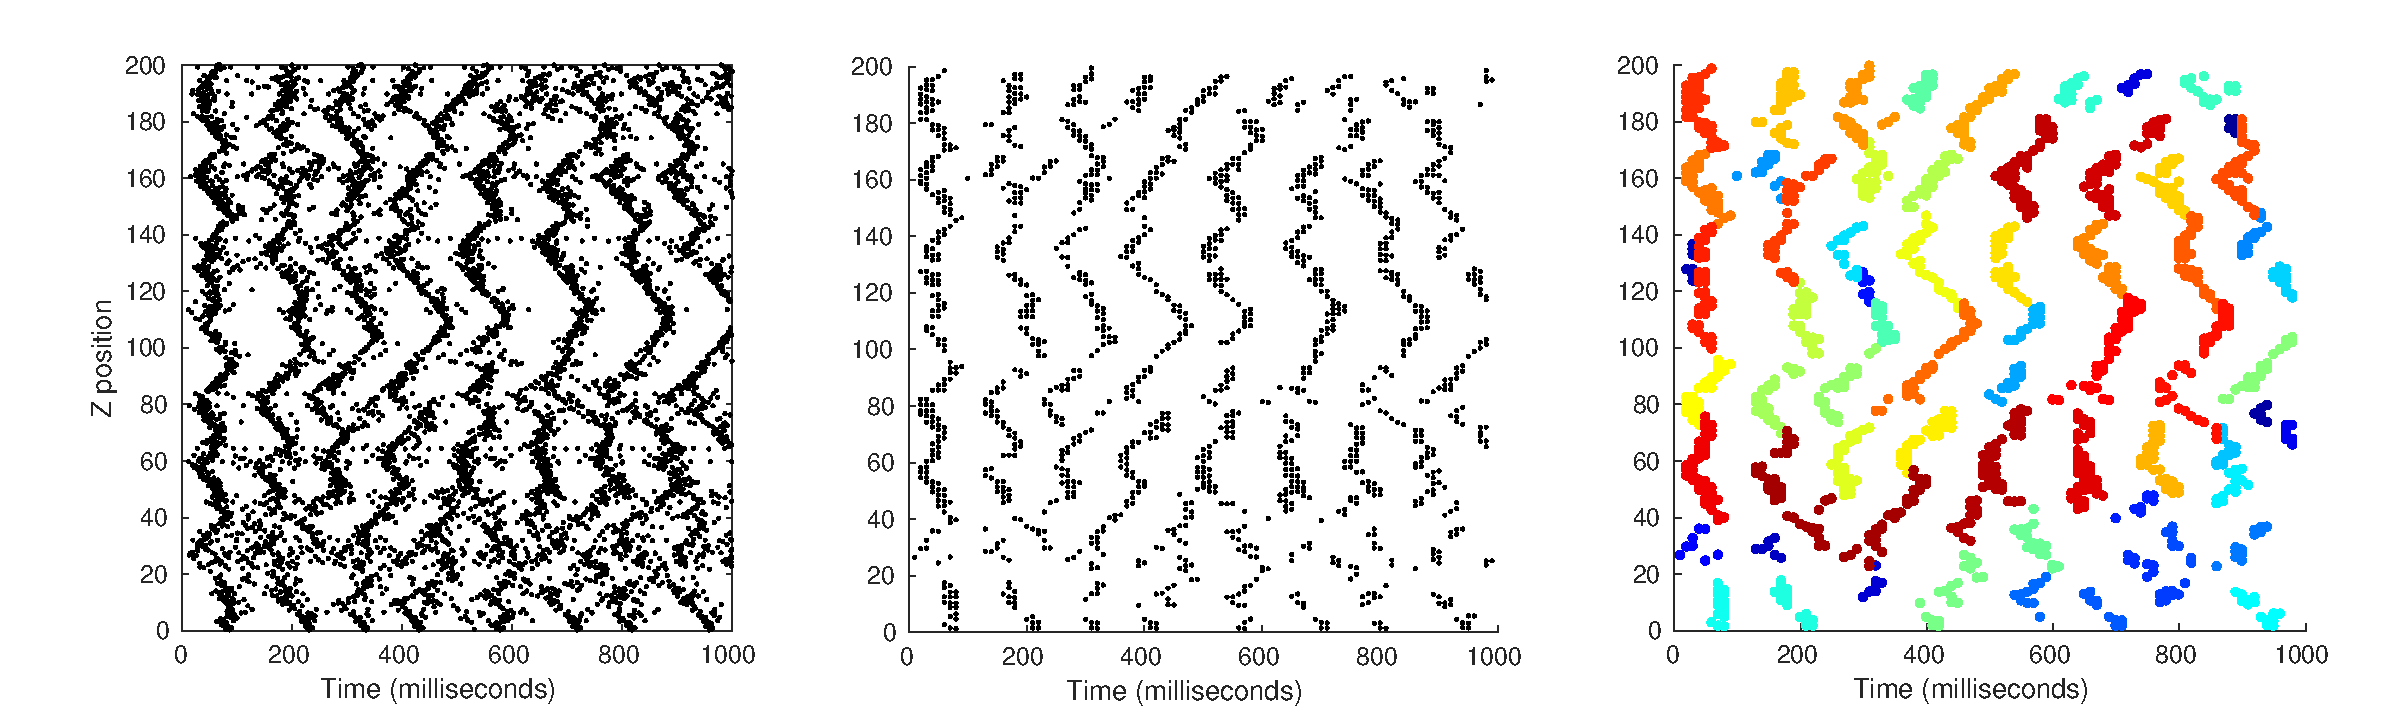
\includegraphics[width=\textwidth]{fig/DetectorExample}
 \caption{Wave identification and labeling using an example SCE with dimensions 2x2x200 . Left: Raster plot of firing events where dots represent neuronal action potentials. 
          Traveling waves can be seen as diagonal structures of dense firing activity. 
          Center: The clustering operation removes background spikes. 
          Right: Individual waves are labeled with unique identifiers color coded in the figure.}
 \label{fig:wave_analysis}
\end{figure}

Our wave detection and analysis approach must remain valid across a range of model parameters. 
We show sample visualizations for varying values of $K$ in Figure \ref{fig:detector_test}.
This detector test demonstrates that our detection and analysis method detects and labels traveling waves of various lengths even in a noisy background.
\begin{figure}[!htb]
 \caption{The clustering and wave labeling process. Spike raster plot (left), filtered clusters (middle) and labeled waves (right, each color is a unique wave) are shown for SCE with different values of $K$. }
 \label{fig:detector_test}
 \centering
   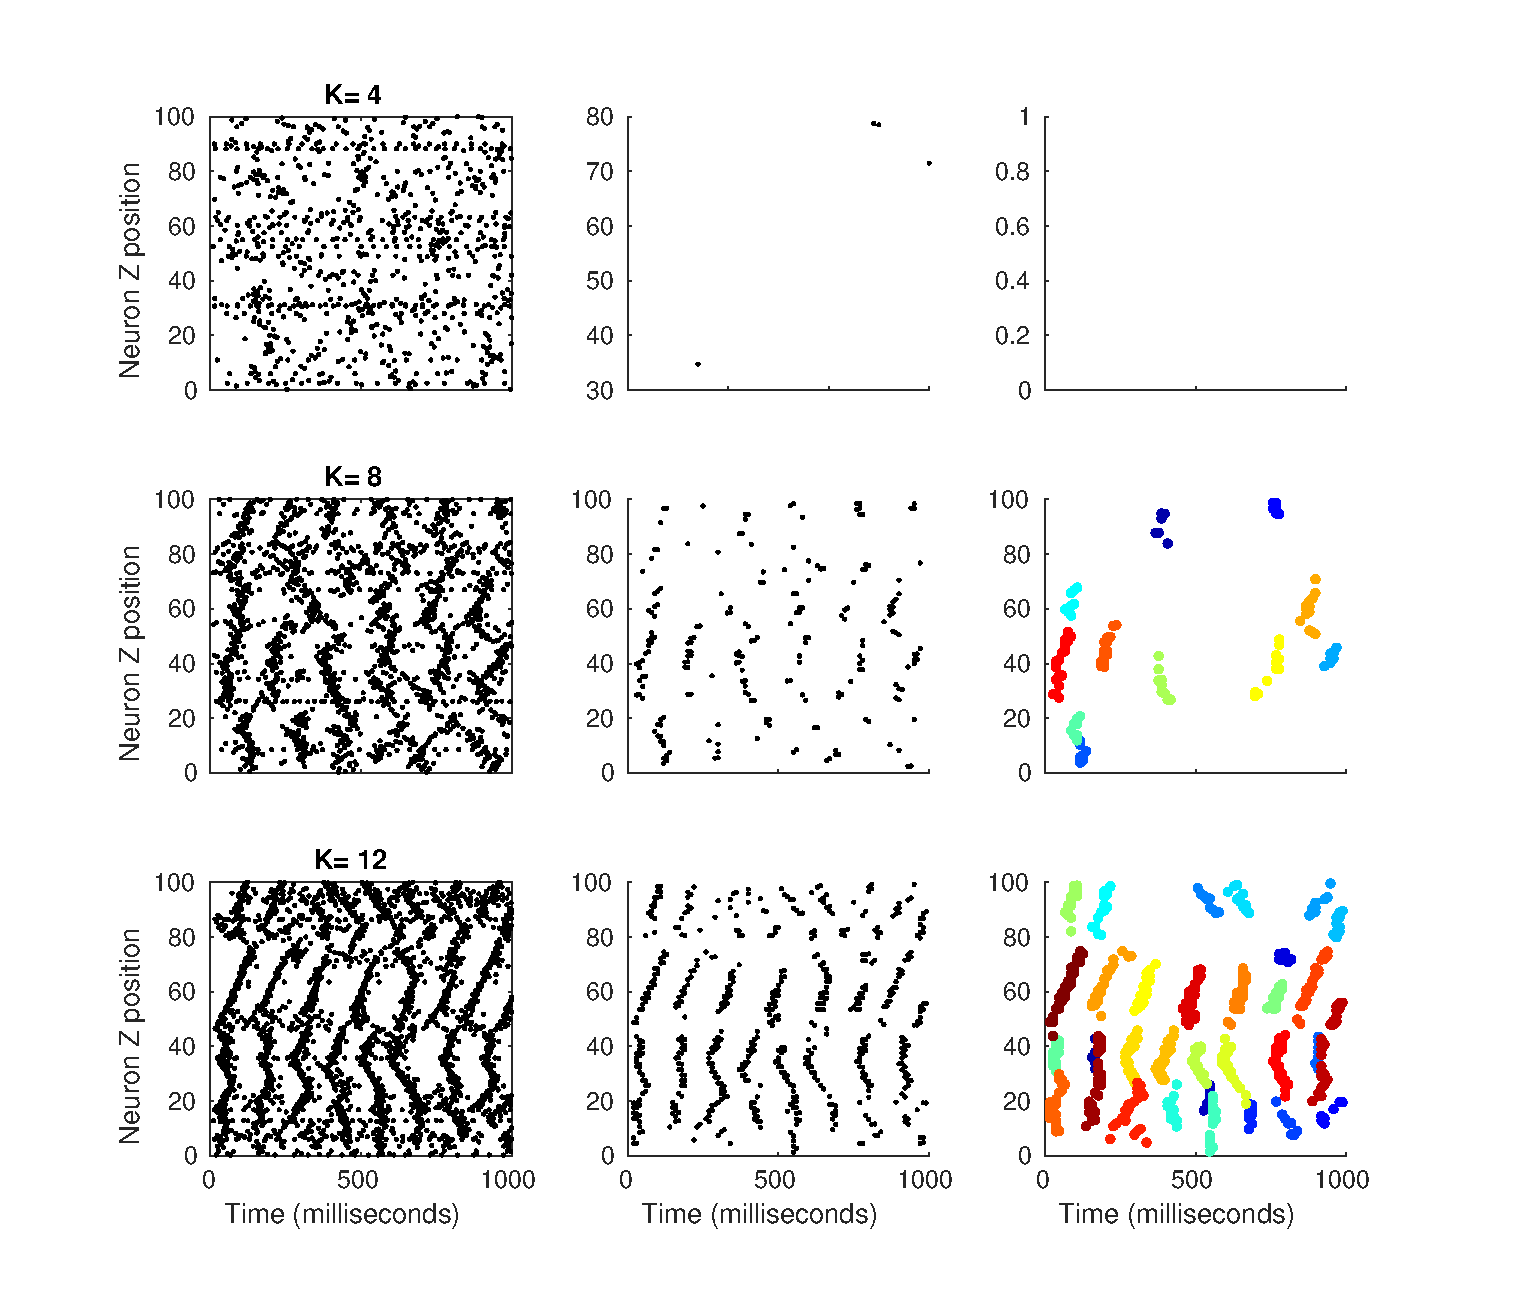
\includegraphics[width=\textwidth]{fig/DetectorTest}
\end{figure}

\FloatBarrier
Once identified and labeled, we measure wave propagation speeds and wave initiation locations. 
We also measure the "wave firing fraction" defined as the fraction of spikes that are associated with the labeled traveling wave (total number of spikes found within the waves divided by number of spikes in the simulation). 

Our exploration of the behavior of traveling waves in an SCE involves testing properties of these waves as a function of the different parameters of our model.
For determining existence of traveling waves we use a $2x2x100$ SCE  with background stimulation (Eq \ref{eq:randomstim}) and vary parameters around a neighborhood of the reference point $\Sigma = \{K=10,\lambda=2.5,P_{exc}=0.8,\kappa=1.0 \}$ that we have determined can sustain traveling waves.
To measure wave propagation speed we use a $2x2x50$ SCE with  a step stimulus applied to the lowest layers of the SCE and adjust our reference point to be $\Sigma_v = \{K=24,\lambda=2.5,P_{exc}=0.8,\kappa=1.0 \}$.
This reference point was selected after inspecting the SCE behavior under a wide range of parameter values.
The increase in $K$ is required when using the step stimulus because the higher layers of the SCE do not receive any stimulus.
This requires stronger connections so that the traveling wave can elicit spikes from neurons resting at equilibrium.

\FloatBarrier

\endinput
%%
%% End of file `example-1.tex'.

%%
%% This is file `example-1.tex',
%% generated with the docstrip utility.
%%
%% The original source files were:
%%
%% drexel-thesis.dtx  (with options: `example-part')
%% 
%% This is a generated file.
%% 
%% Copyright (C) 2010 W. Trevor King
%% 
%% This file may be distributed and/or modified under the conditions of
%% the LaTeX Project Public License, either version 1.3 of this license
%% or (at your option) any later version.  The latest version of this
%% license is in:
%% 
%%    http://www.latex-project.org/lppl.txt
%% 
%% and version 1.3 or later is part of all distributions of LaTeX version
%% 2003/06/01 or later.
%% 

\chapter{Quasi 1-D Minicolumns}
Traveling waves in one-dimensional neuronal systems have been previously explored using several theoretical methods.
In the literature on neural fields \citep{Ermentrout1979}\citep{Folias2012} and coupled oscillators \citep{Kopell1986}\citep{Williams1997} isotropic networks of homogeneous neurons with symmetric synaptic coupling give rise to field models which exhibit traveling wave solutions for certain parameter values. 
One-dimensional waves have also been observed in simulations using firing rate neurons \citep{Roxin2005}, integrate-and-fire neurons \citep{Bressloff1997}\citep{Golomb1999} and Hodgkin-Huxley neurons \citep{Golomb1997}.
\citet{Senk2020} used populations of both rate neurons and integrate-and-fire neurons and developed a method to translate parameters between the two different models.
These simulations again use homogeneous neuronal populations in networks that are invariant to spatial translation, resulting naturally in periodic spatio-temporal patterns.
These purely one-dimensional systems may not be robust to realistic variation in neuron properties, connectivity and noise.
This is exemplified in \citet{Senk2020} where traveling waves are only observed for certain parameter values, and \citet{Strogatz1991} where the stability of systems of coupled oscillators can be radically altered by including infinitesimal noise.
Our current work explores traveling waves in quasi-one-dimensional networks with substantial randomness in both individual neurons (randomly selecting type and randomizing dynamical parameters), connectivity between neurons, and stimulus to the neurons.

Previous studies have used one-dimensional structures largely for their computational or analytic simplicity. 
Consideration of a quasi one-dimensional system may seem as an unnecessary complication, but there is no a priori reason that quasi one-dimensional traveling waves may not be found in vivo.
Of interest, there are regions of the brain where there are what seem to be quasi  one-dimensional structures \citep{buxhoeveden2002}\citep{mountcastle1997} typically called micro- or minicolumns. 
These minicolumns are aligned perpendicular to the pia and can be hundreds of microns long.  
Although their relevance to cognition and function is still being debated \citep{horton2005}\citep{Cruz2009}\citep{buxhoeveden2002}, it is possible that they can sustain traveling waves.

To address this possibility, here we investigate the conditions under which traveling waves can exist on quasi one-dimensional systems, and their fundamental properties and dynamics.  
Inspired by minicolumns, our systems consist of thin (few neuron) and long (~100 neuron) networks of locally connected neurons placed on a three-dimensional lattice.  
We model the neuron dynamics using the Izhikevich model \citep{izhikevich2003} that allow us to explore more complex neuron dynamics than typically afforded by integrate-and-fire models \citep{keane2015}\citep{Senk2020} while also providing a distribution of neuron dynamical parameters that mimics the type and variety of neurons observed in the mammalian cortex.
We use a morphology and connectivity model inspired by \citet{maass2002},incorporating a local connectivity model \citep{Levy2012}\citep{Pyle2017}\citep{Fino2011}.
To incorporate elements of a real brain, we consider a model with substantial randomness in both individual neurons and connections between neurons while also considering  distance-dependent time delays in the propagation of action potentials.

Among our main findings we determine parameters in our model that allow for the generation of traveling waves in our quasi one-dimensional systems. 
These traveling waves exhibit properties such as spontaneous creation from a random background stimulus, annihilation of colliding waves, and a wave velocity that is determined by both the propagation speed of the action potential and the neuron dynamics.
Traveling waves are present in both locally-connected and fully-connected systems. 
The traveling waves in fully connected systems are dependent upon the action potential propagation speed, while traveling waves can propagate in locally-connected systems even when action potential propagation is instantaneous.

The results are organized as a series of computational experiments on traveling waves.
We first determine which parameterizations of our model support traveling waves.
Stronger and more numerous local connections between neurons are found to facilitate the formation of traveling wave patters.
We then investigate the influence of neuron dynamics and connectivity on the speed of traveling waves.
Stronger neuronal connections and faster action potential propagation are shown to increase traveling wave speed, but the neuron dynamics enforce an upper limit on the speed. 
Low-threshold-spiking inhibitory neurons are shown to consistently generate traveling waves through the mechanism of post-inhibitory rebound spiking.
The low-threshold-spiking inhibitory neurons also suppress traveling waves that originate from other points in the SCE.
Finally, we examine fully-connected networks and observe that traveling wave patterns can still emerge provided the action potential propagation speed is slow enough.

\section{Minicolumn structure}
We use open boundary conditions, so neurons near the ends of the SCE will have fewer connections than those in the middle.
An example of an SCE showing the connectivity structure is shown in Figure \ref{fig:column_structure}.
\begin{figure}[!htb]
 \caption{Example SCE with dimensions 2x2x10 (XxYxZ), $\lambda$=2.5, and C=1. A)  SCE showing connections between neurons as lines colored using a color scale that indicates the connection length. 
 B)  Connection matrix. E-E connections are green, E-I are black and both I-E and I-I  are red. 
 The labels of the neurons used in both axes are sequentially assigned starting at the bottom (Z=0).
 C) The sum of presynaptic weights for each neuron shows the anisotropy of this model, with substantial variation in input strength and sign between the neuron inputs.}
 \label{fig:column_structure}
 \subfloat[][]{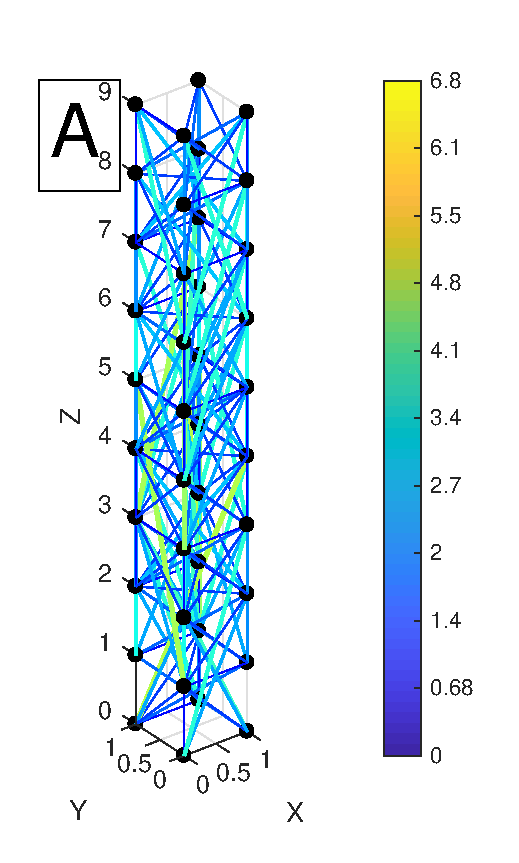
\includegraphics[height=60mm]{fig/column_structure_A}}
 \subfloat[][]{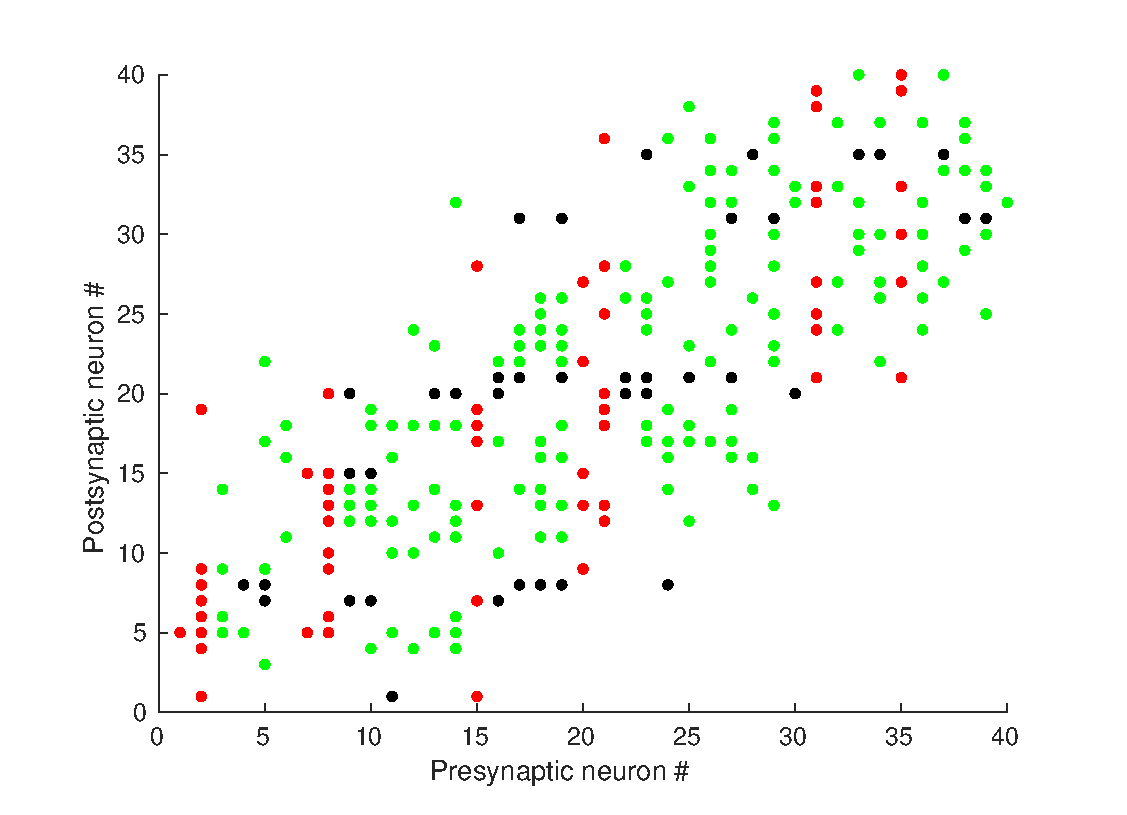
\includegraphics[height=60mm]{fig/column_structure_B}}
 \subfloat[][]{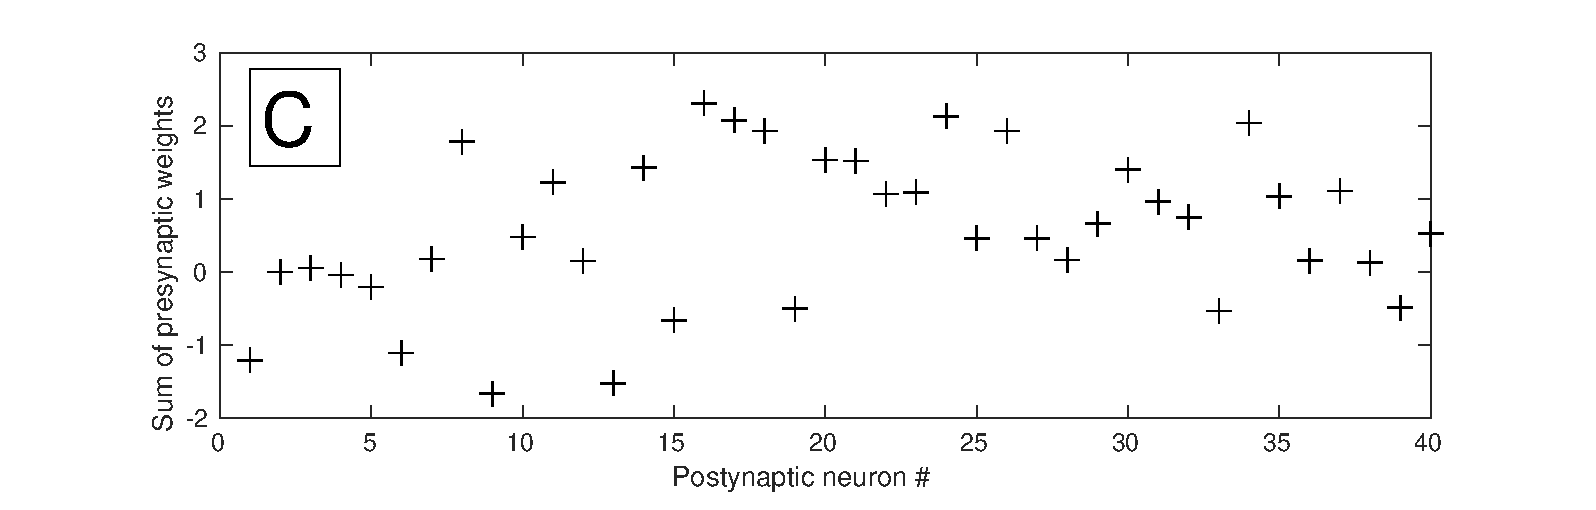
\includegraphics[width=\textwidth]{fig/column_structure_C}}
\end{figure}

A crucial element in neuronal systems is the existence of time delays between the creation of a presynaptic action potential and the arrival of that spike to a target neuron. 
We use distance-dependent time delays for the propagation of a spike from neuron $i$ to neuron $j$ of $\tau_{ij} = \kappa  D(i,j)$. 
The constant of proportionality $\kappa$ ranges from $0$ to $4$.
When $\kappa=0$ the action potential excites the post-synaptic neuron on the succeeding simulation time step.
 
The distribution of post-synaptic connections and delay times are shown in Figure \ref{fig:connection_delay_distrbution} for an example minicolumn.
\begin{figure}[!htb]
 \caption{Distribution of (A) number of post-synaptic connections per neuron and (B) delay time. Data was taken over 100 realizations of a 2x2x50 SCE, $\lambda=2.5$, $\kappa=1$.  } 
     \subfloat[][]{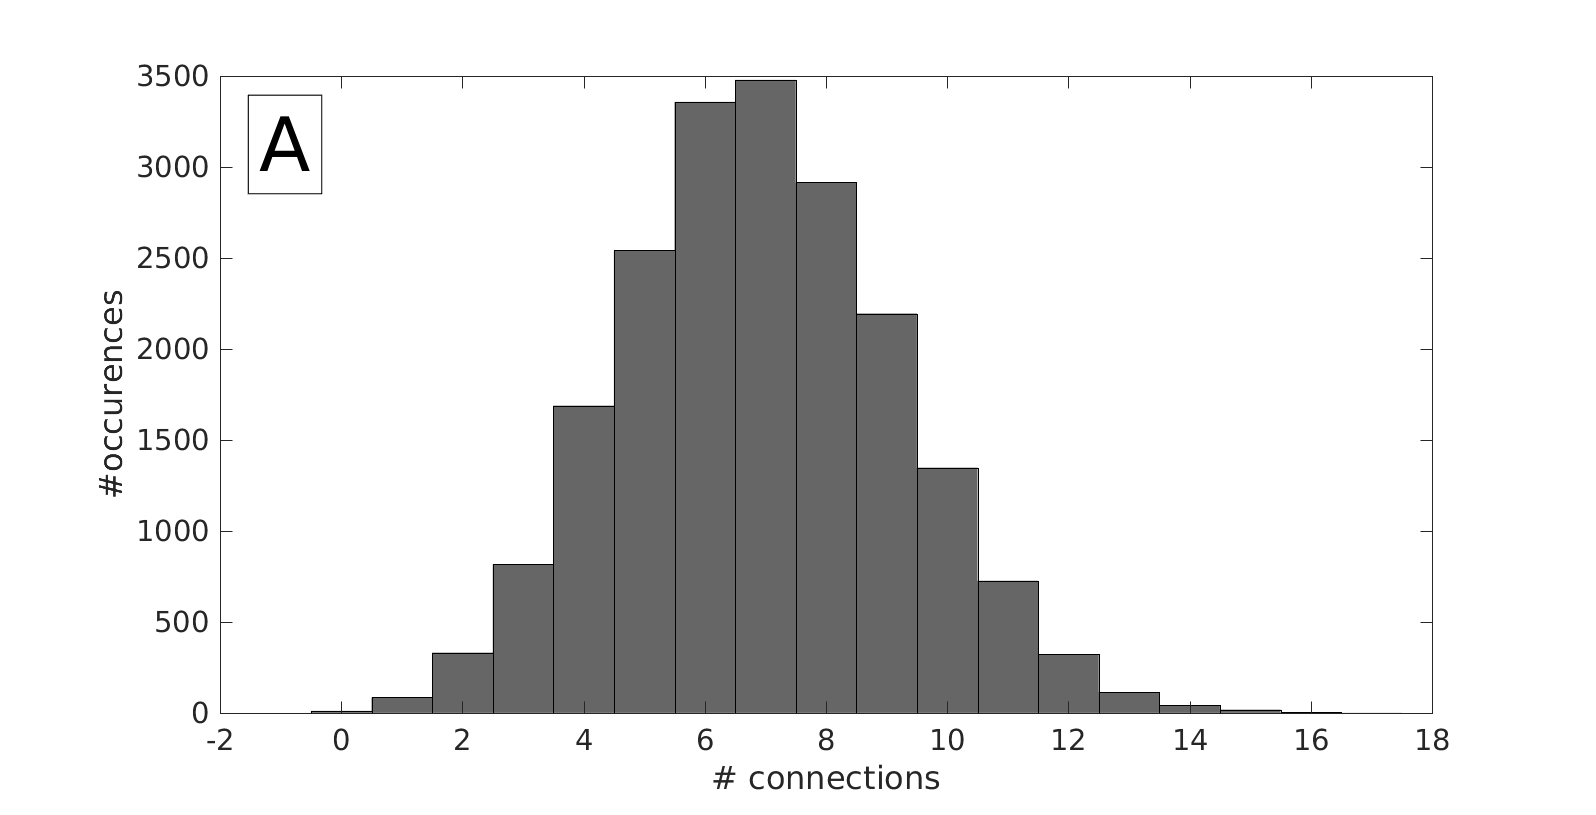
\includegraphics[width=\textwidth]{fig/ConnectionNumberDistribution} }
     \subfloat[][]{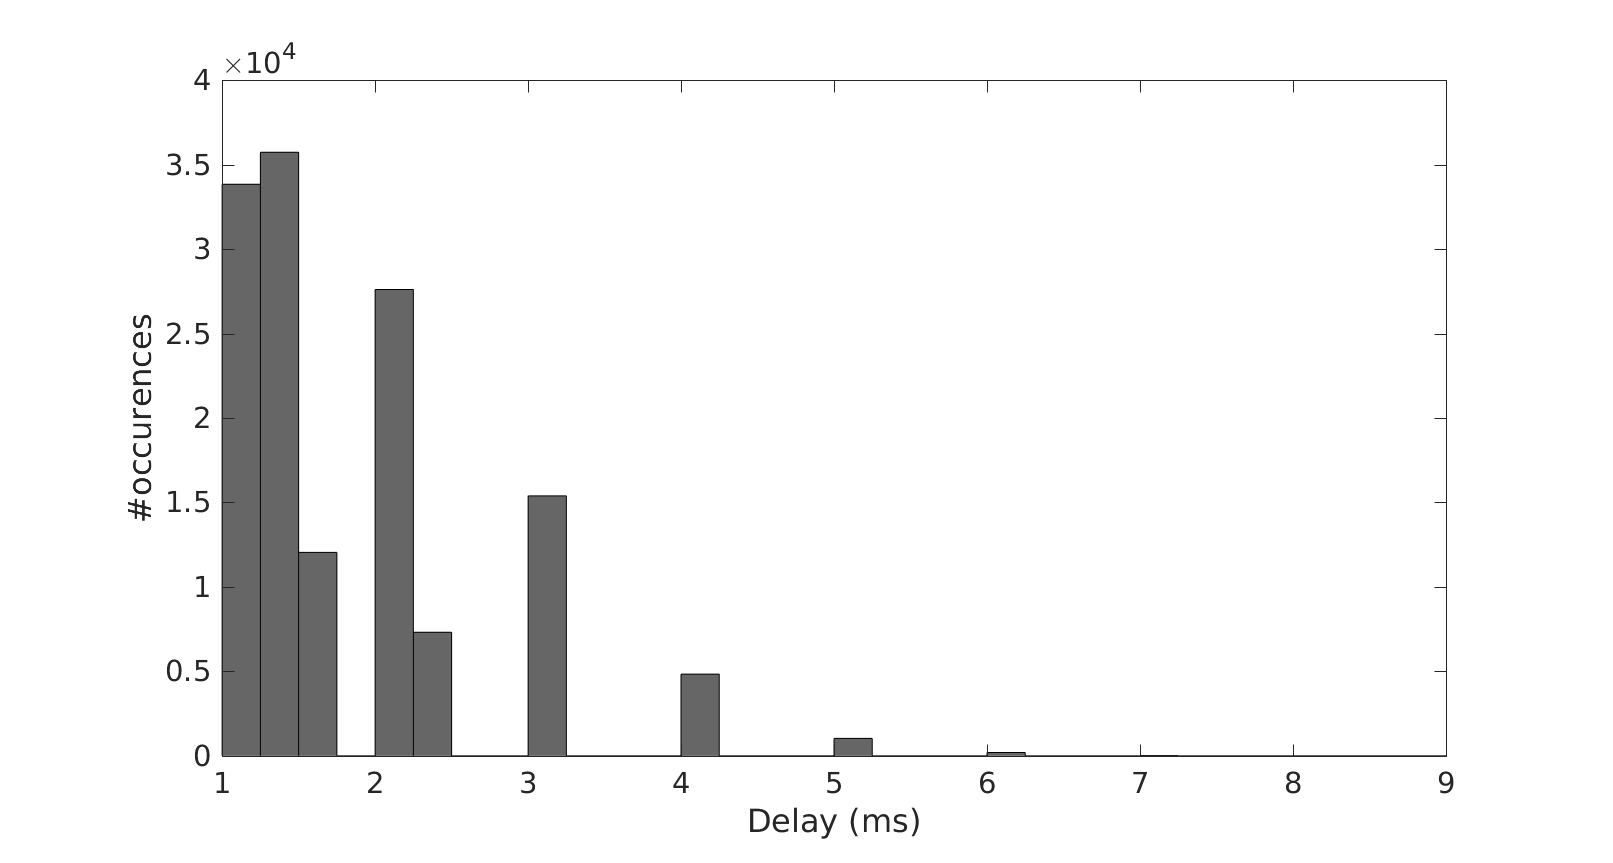
\includegraphics[width=\textwidth]{fig/DelayDistribution} }
 \label{fig:connection_delay_distrbution}
\end{figure}
 \FloatBarrier
 
For every simulation we record all of the spikes from all neurons. 
We visualize the spikes in spike raster plots (e.g. Figure \ref{fig:sigma_raster} ).
Because here we focus on traveling waves in the Z direction, we plot the spikes according to the Z position of the neurons.
As a consequence, at each Z position there are multiple neurons that could contribute to the spike raster plot at that Z coordinate (e.g. 4 neurons for the X=2, Y=2 SCE case).

To automatically identify waves we perform a spatial clustering operation to this data to identify spatiotemporal regions identified by high firing density. 
The clustering operation produces an output cluster for any group of more than $3$ spike events that fall within a $20ms$ time window from neurons that are no more than $3$ layers apart.
Each cluster $C(t,z)$ has a time $t$ and position $z$.
This clustering removes random background firing activity. 
The waves are identified using a plane sweep algorithm that proceeds along the dimension of simulation time and applies wave labels to clusters such that all clusters with the same label are part of the same wave.
When a new cluster $C(t,z)$ is encountered, the algorithm associates $C(t,z)$ with any existing wave if the existing wave has a cluster $C(t_c,z_c)$ within $40 ms$ and $6$ units of the new cluster.
If there is no such adjacent cluster a new wave is created using $C(t,z)$ as the first cluster.

An example of the clustering and identification is shown in Figure 2, with further illustration in SI Figure 1.
\begin{figure}[!htb]
 \centering
 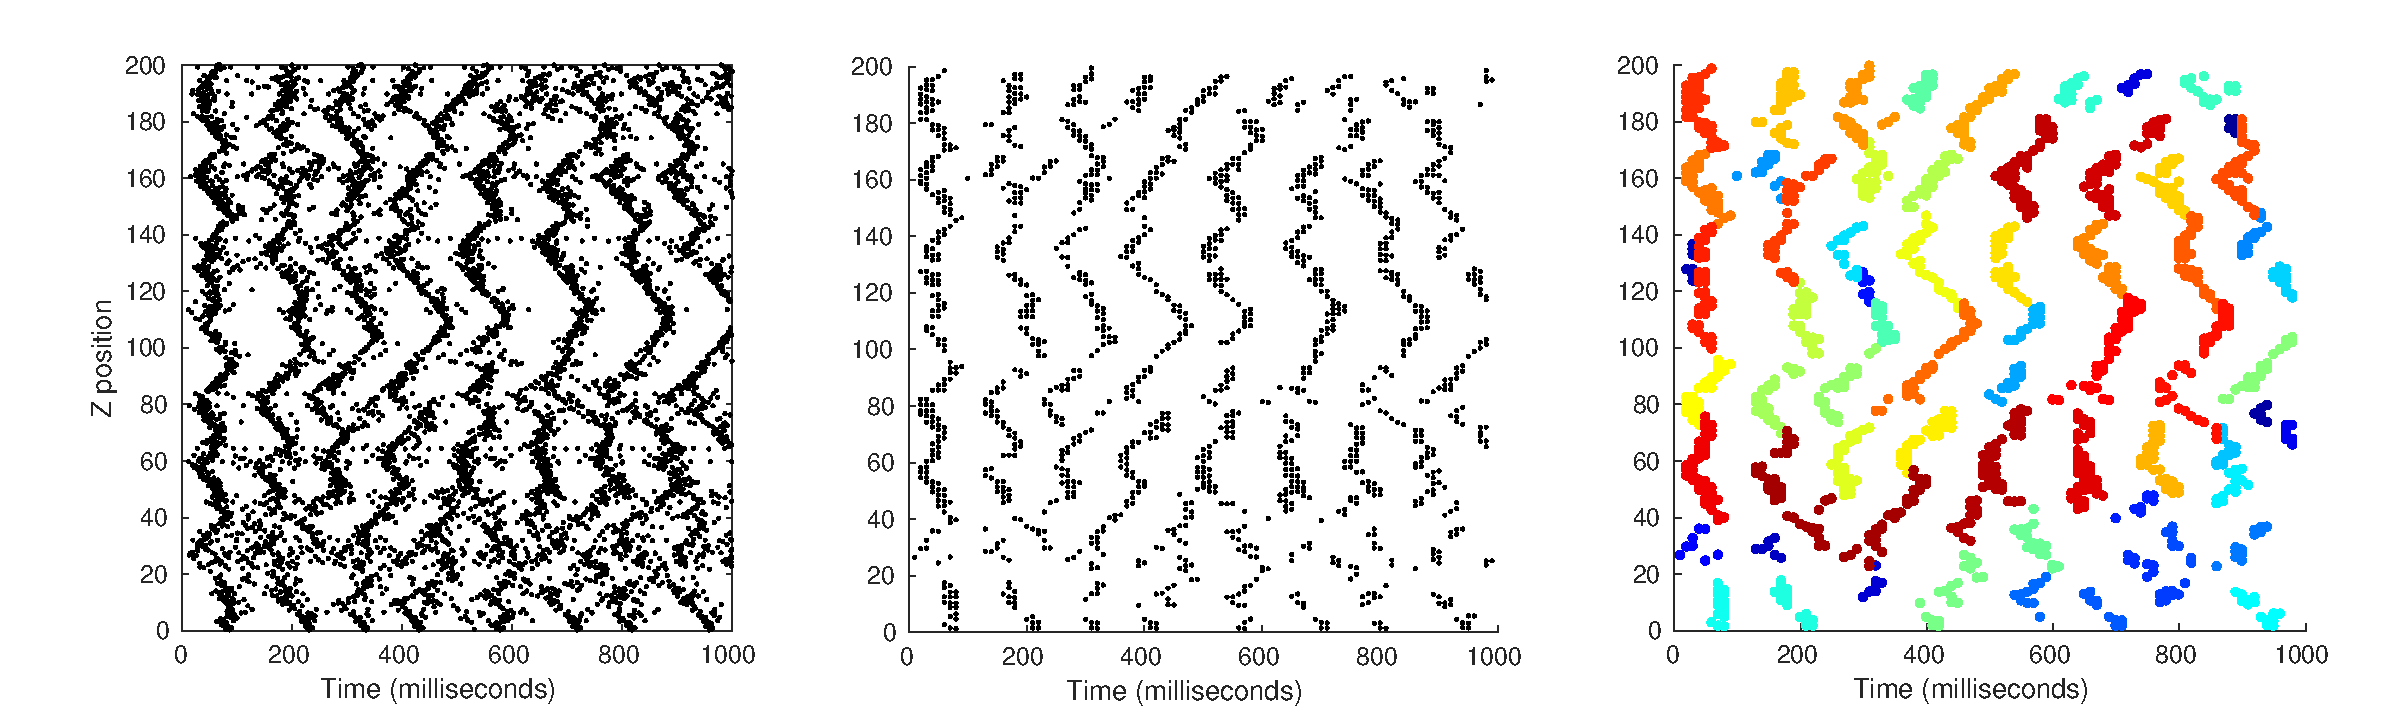
\includegraphics[width=\textwidth]{fig/DetectorExample}
 \caption{Wave identification and labeling using an example SCE with dimensions 2x2x200 . Left: Raster plot of firing events where dots represent neuronal action potentials. 
          Traveling waves can be seen as diagonal structures of dense firing activity. 
          Center: The clustering operation removes background spikes. 
          Right: Individual waves are labeled with unique identifiers color coded in the figure.}
 \label{fig:wave_analysis}
\end{figure}

Our wave detection and analysis approach must remain valid across a range of model parameters. 
We show sample visualizations for varying values of $K$ in Figure \ref{fig:detector_test}.
This detector test demonstrates that our detection and analysis method detects and labels traveling waves of various lengths even in a noisy background.
\begin{figure}[!htb]
 \caption{The clustering and wave labeling process. Spike raster plot (left), filtered clusters (middle) and labeled waves (right, each color is a unique wave) are shown for SCE with different values of $K$. }
 \label{fig:detector_test}
 \centering
   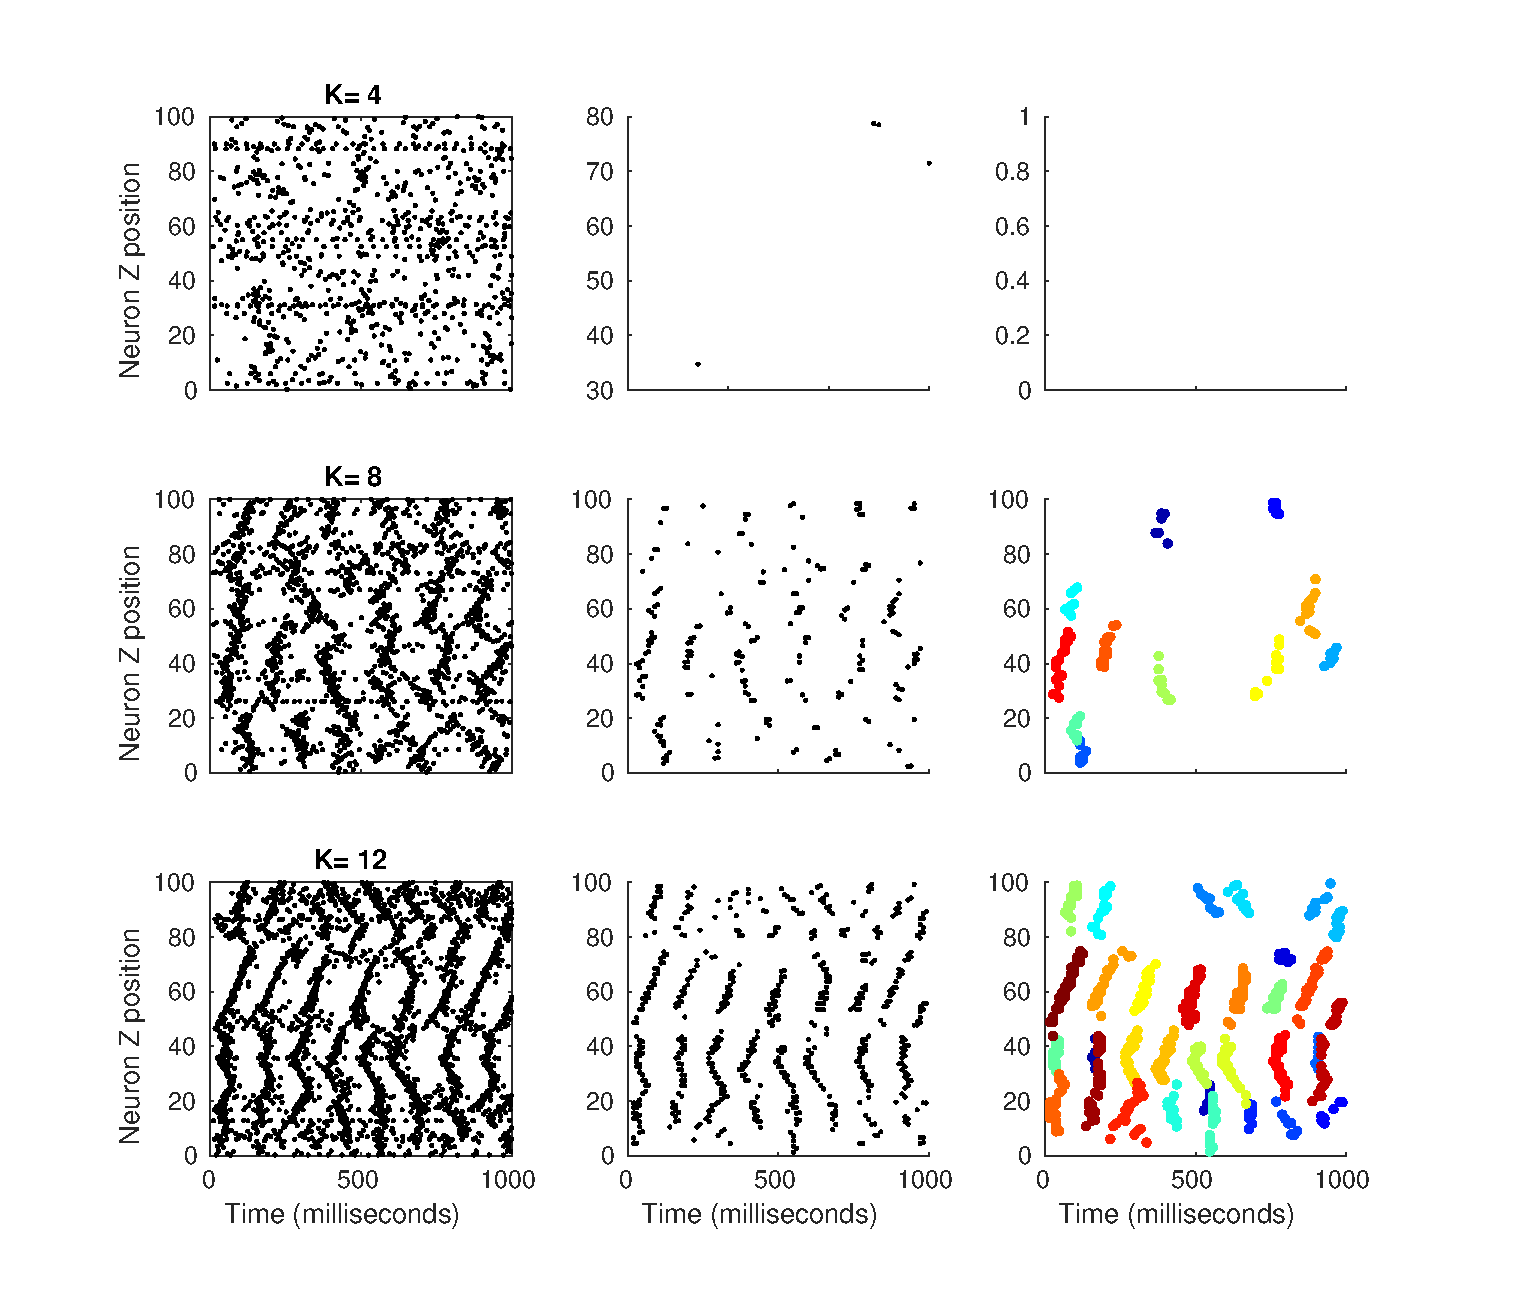
\includegraphics[width=\textwidth]{fig/DetectorTest}
\end{figure}

\FloatBarrier
Once identified and labeled, we measure wave propagation speeds and wave initiation locations. 
We also measure the "wave firing fraction" defined as the fraction of spikes that are associated with the labeled traveling wave (total number of spikes found within the waves divided by number of spikes in the simulation). 

Our exploration of the behavior of traveling waves in an SCE involves testing properties of these waves as a function of the different parameters of our model.
For determining existence of traveling waves we use a $2x2x100$ SCE  with background stimulation (Eq \ref{eq:randomstim}) and vary parameters around a neighborhood of the reference point $\Sigma = \{K=10,\lambda=2.5,P_{exc}=0.8,\kappa=1.0 \}$ that we have determined can sustain traveling waves.
To measure wave propagation speed we use a $2x2x50$ SCE with  a step stimulus applied to the lowest layers of the SCE and adjust our reference point to be $\Sigma_v = \{K=24,\lambda=2.5,P_{exc}=0.8,\kappa=1.0 \}$.
This reference point was selected after inspecting the SCE behavior under a wide range of parameter values.
The increase in $K$ is required when using the step stimulus because the higher layers of the SCE do not receive any stimulus.
This requires stronger connections so that the traveling wave can elicit spikes from neurons resting at equilibrium.

\FloatBarrier

\section{Existence of 1-D waves} \label{sub:waves}
We first explore which parameterizations of our model will support traveling waves.
We detect the waves as described in Methods, and then use the wave firing fraction metric to determine for which parameter values our model will produce traveling waves.
We fix the connection normalization constant $C$ in equation \ref{eq:connectivity} to $0.5$ and we fix the stimulus strength $M$ in equation \ref{eq:randomstim} to $5$.
For this value of C and $\lambda=2.5$ each neuron has an average of $6.90$ input connections, as measured across $100$ randomly-generated SCE (see SI Figure 2 for connectivity distribution).

The key parameters of our model that we examine are the connection strength $K$, the characteristic connection length $\lambda$, the fraction of excitatory neurons $P_{exc}$ and the delay parameter $\kappa$.
First we establish that traveling waves are observed at the reference  point $\Sigma = \{K=10,\lambda=2.5,P_{exc}=0.8,\kappa=1.0 \}$.
We then vary the individual parameters about $\Sigma$ to examine how they influence traveling wave formation.

At the reference  point $\Sigma$ the average wave firing fraction over 100 trials is found to be $88.6\%$ with a standard deviation of $4.38\%$.
A representative raster plot of the spike events (Figure \ref{fig:sigma_raster}) clearly shows the traveling waves.
\begin{figure}[!htb]
 \centering
 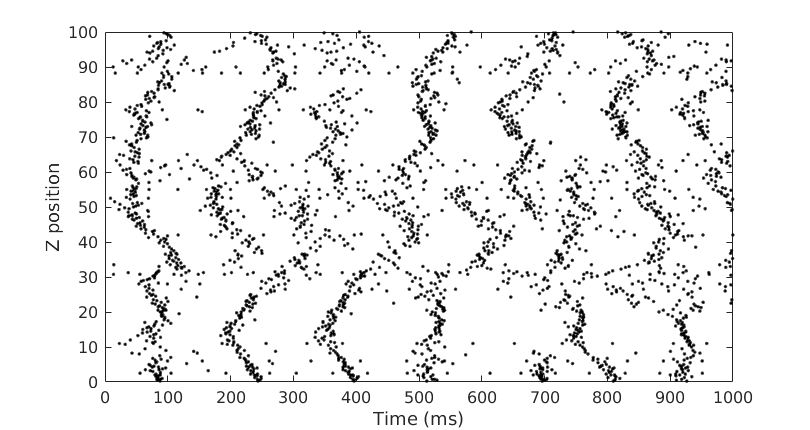
\includegraphics[width=0.75\textwidth]{fig/baseline}
 \caption{Raster plot of neuron firing events over time. The model parameters are at the reference  point $\Sigma$. Each dot represents the spike-time emission of a neuron. Traveling waves can be seen as diagonal structures of dense firing activity \citet{Senk2020}. }
 \label{fig:sigma_raster}
\end{figure}

The effect of varying the parameters on traveling waves are shown in Figure \ref{fig:wave_parameters}.
The graphs of the wave firing fraction versus $K$, $\lambda$ and $P_{exc}$ show similar behavior.
Traveling waves are not supported for low values of these parameters.
As the parameter values increase traveling waves emerge, and as the parameters grow large the traveling waves dominate the firing activity.
Stronger connections ($K$) or more numerous connections ($\lambda$) makes it easier for firing activity to spread to adjacent neurons.
A higher excitatory fraction acts similarly to a higher connection strength. 
As the presynaptic activity to each neuron is more excitatory and less inhibitory, it is easier for the traveling wave to propagate.
These data suggest that these three parameters all work towards strengthening the local neighborhood of neurons and facilitating the propagation of coordinated spikes as traveling waves.

\begin{figure}[!htb]
 \centering
 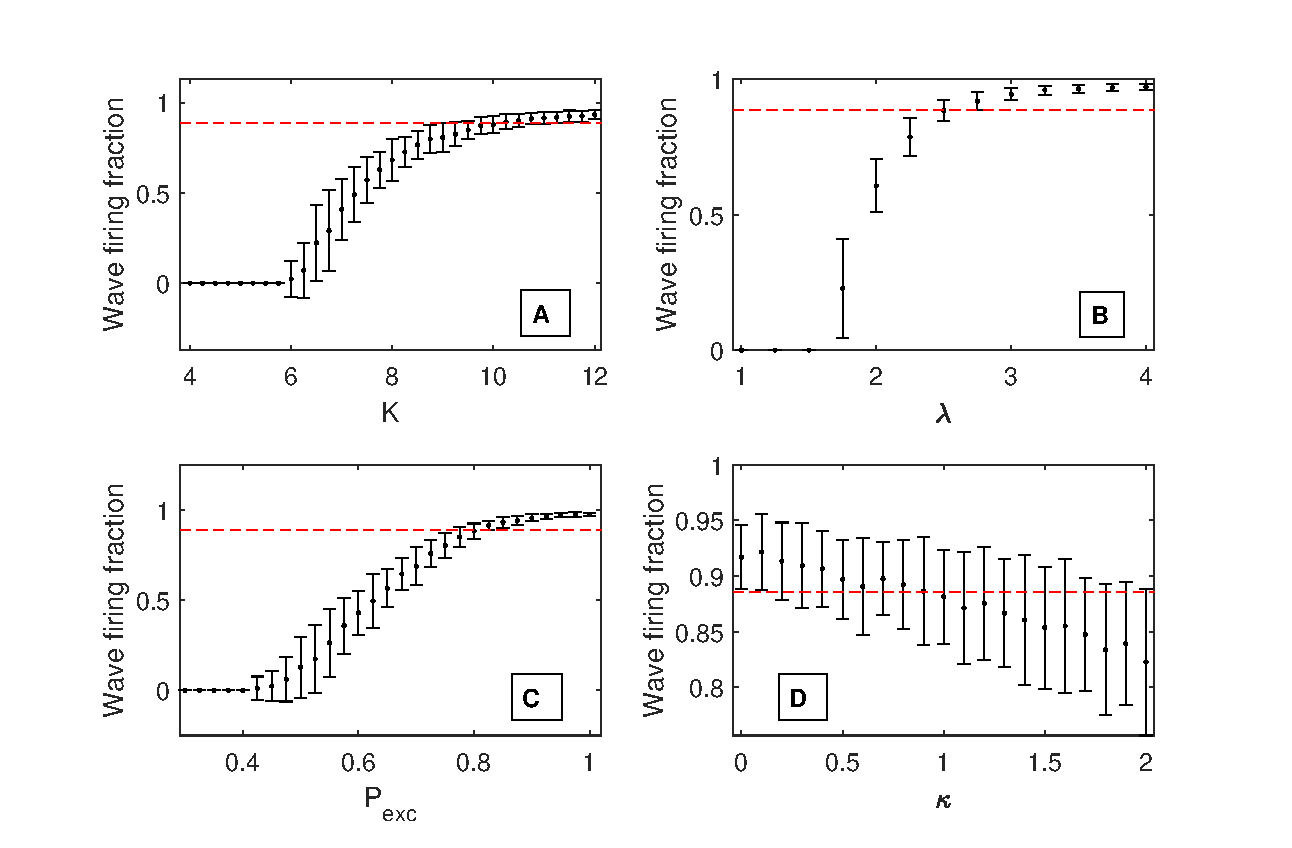
\includegraphics[width=\textwidth]{fig/ParamWaveSim}
 \caption{Onset of traveling waves as a function of model parameters in the neighborhood of $\Sigma$ (100 trials for each parameter value, error bars $1\sigma$). 
         The dashed red lines show the wave firing fraction at the reference  point $\Sigma$.  
         Varying each individual parameter while holding the other parameters at their $\Sigma$ values, we observe onset of traveling waves at $K=6$ (A), $\lambda=1.5$ (B), and $P_{exc}=0.45$ (C).  
         D) Traveling waves are present at all values of $\kappa$. }
 \label{fig:wave_parameters}
\end{figure}

\FloatBarrier

For the range of values tested, the parameter $\kappa$ does not show a strong influence on the existence of traveling waves. 
This is in contrast to previous work in largely isotropic networks and neural field models which found that the delay parameter is important for the emergence of traveling waves \citet{Senk2020}\citet{Atay2006}\citet{Roxin2005}.
However, it is consistent with other work that found traveling wave patterns without including propagation delay \citet{Folias2012}\citet{Wyller2007}.

A natural question is whether the few long connections along the Z direction that cannot exist in the X or Y directions exert a dominant role on these results.
By performing the same experiments as in Figure 4, but now pruning long-range connections, results show that the influence of the longer connections is minimal (SI Figure 4).

We establish purely one-dimensional systems in our model for comparison to previous work with purely one-dimensional systems.
We start with the SCE described in Section 3.1 for measuring wave speed: a 2x2x50 (XxYxZ) SCE with model parameters at the reference point $\Sigma_v$. 
While previous work with this SCE measured the speed of the waves, here we determine the existence of traveling waves based on whether the neurons in the top layer of the SCE fire.
\textbf{The baseline quasi one-dimensional SCE creates 74 traveling waves in 100 trials}, where each trial is a random draw on all randomized parameters in the model and stimulus.
An example raster plot is shown in Figure \ref{fig:OneDimensionalRasterPlots}A.

We create a purely one-dimensional version of this SCE with X=1 and Y=1 and all other model parameters at $\Sigma_v$.
\textbf{No traveling waves are observed in this SCE in 100 trials}. 
An example raster plot is shown in Figure \ref{fig:OneDimensionalRasterPlots}B.
We then modify this purely one-dimensional SCE by increasing $\lambda$ from $2.5$ to $4$ and increasing $K$ from $2$4 to $30$.
These parameters represent the highest connectivity and connection strength tested in our quasi one-dimensional SCE.
\textbf{We still do not observe any traveling waves in 100 trials} of this SCE with enhanced connectivity and connection strength.
An example raster plot is shown in Figure \ref{fig:OneDimensionalRasterPlots}C.

Finally we look to remove the random elements of our model to make it more comparable to previous work.
We set $C=1.0$ to create a more uniform and isotropic connectivity between the neurons.
We set $P_{exc}=1$ so that all neurons are excitatory with no inhibitory neurons at random locations.
We remove all random factors from the Izhikevich model parameters a, b, c and d (Table 1).
All neurons therefore have identical dynamics.
\textbf{With this more uniform model we observe 98 traveling waves in 100 trials}, reproducing previous results that have found traveling waves in purely one-dimensional networks.
An example raster plot is shown in Figure \ref{fig:OneDimensionalRasterPlots}D.
Although we have removed most variation from this SCE, the two trials with no waves are not unexpected as the stimulus is still randomized and the connectivity is still probabilistic (see Equation 1).

\begin{figure}[!htb]
 \caption{ Example raster plots of the SCE used for comparison to previous work in purely one-dimensional systems.
           A) The 2x2x50 SCE with model parameters at $\Sigma_v$ supports traveling waves along the entire SCE. 
	   B) The 1x1x50 version of the same SCE does not exhibit traveling waves.
	   C) Even with $K$ increased from $24$ to $30$ and $\lambda$ increased from $2.5$ to $4$, the 1x1x50 SCE still does not support traveling waves.
	   D) Once the random parameters are removed, the 1x1 SCE does support traveling waves. }
   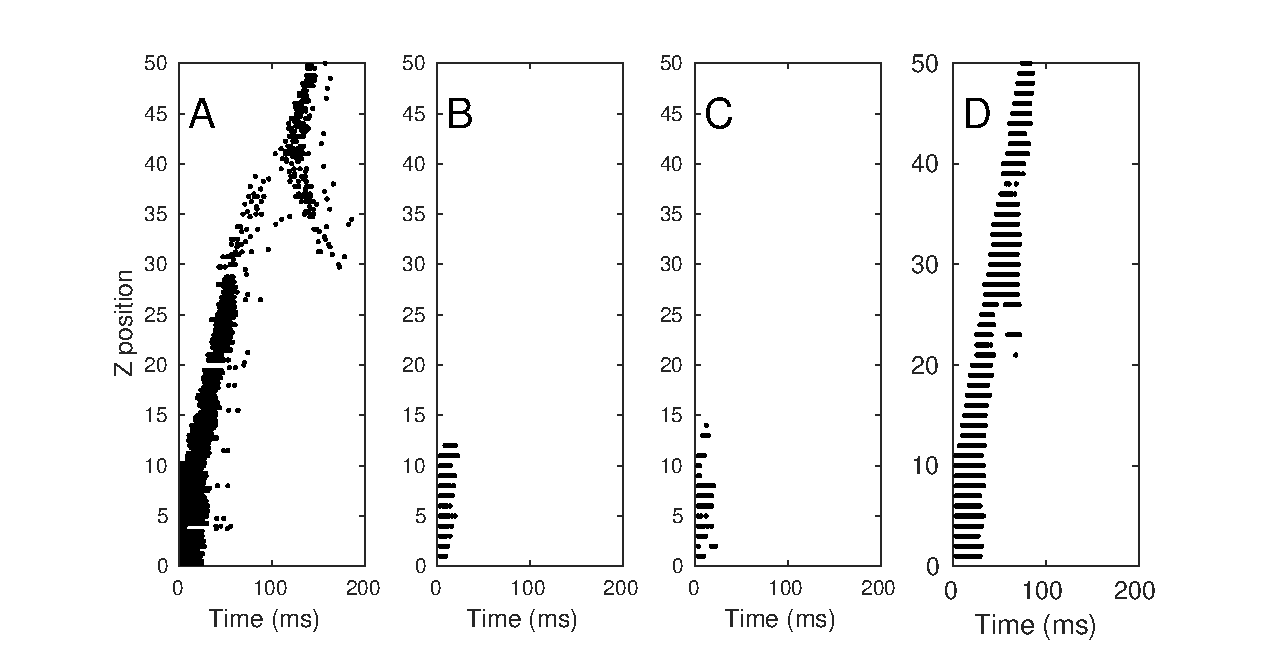
\includegraphics[width=\textwidth]{fig/OneDimensionalComparison_RasterPlots}
   \label{fig:OneDimensionalRasterPlots}
\end{figure}
\FloatBarrier

\section{Wave propagation speed} \label{sub:propagation_speed}
Cortical traveling waves have been observed with propagating speeds from less than $0.1$ to more than $0.8$ meters per second \citet{Sato2012}\citet{Golomb1997}\citet{Chervin1988}.
This is consistent with the action potential propagation speeds in the gray matter of the cortex \citet{Muller2018}. 
This suggests that the dynamics of action potential propagation influence wave propagation. 
To consider the possibility of this relationship we incorporate in our model an action potential propagation time proportional to the distance between the neurons.

Action potential velocity may not be the only factor in the traveling wave propagation speed.
In \citet{Golomb1997} the authors neglected action potential propagation in their model of disinhibited cortical slices as they considered their observed wave velocity of $~0.15 m/s$ to be an order of magnitude faster than axon potential propagation.
In \citet{Chervin1988} the authors found an even slower propagation of $0.06-0.09 m/s$ in disinhibited slices of rat cortex.
In  \citet{Markram1997} a latency of $1.7\pm 0.9\ ms$ was observed between injecting a stimulus in one pyramidal neuron and the resulting excitatory post-synpatic potential in an adjacent pyramidal neuron.
This latency is too large to be due solely to axonal propagation alone given the very short distance between the neurons. 
These results indicate that a second key element, namely neuron and synapse dynamics, will also influence wave propagation speed.
Biological neurons and synapses  have complex internal dynamics, and will not fire instantaneously upon receiving a stimulus.
The input may push the neuron's dynamical system out of equilibrium and cause a spike, but the system dynamics take some time to evolve.
Therefore the spike will occur with some delay after the stimulus.
This is a common behavior in any multidimensional model of neuron dynamics, but it is not captured by the leaky integrate-and-fire model used in much of the previous research \citet{keane2015}\citet{Senk2020}.
As an example, Figure \ref{fig:delay_neuronstep} shows the delayed response of a neuron to a pulse of current using the Izhikevich model.
\begin{figure}[!htb]
 \caption{ A pulse of voltage (bottom) with magnitude $2 mV$, starting at $t=100 ms$ and lasting $2 ms$ disturbs the equilibrium membrane potential of a neuron (top), eliciting a spike at $t=112 ms$. }
 \label{fig:delay_neuronstep}
 \centering
   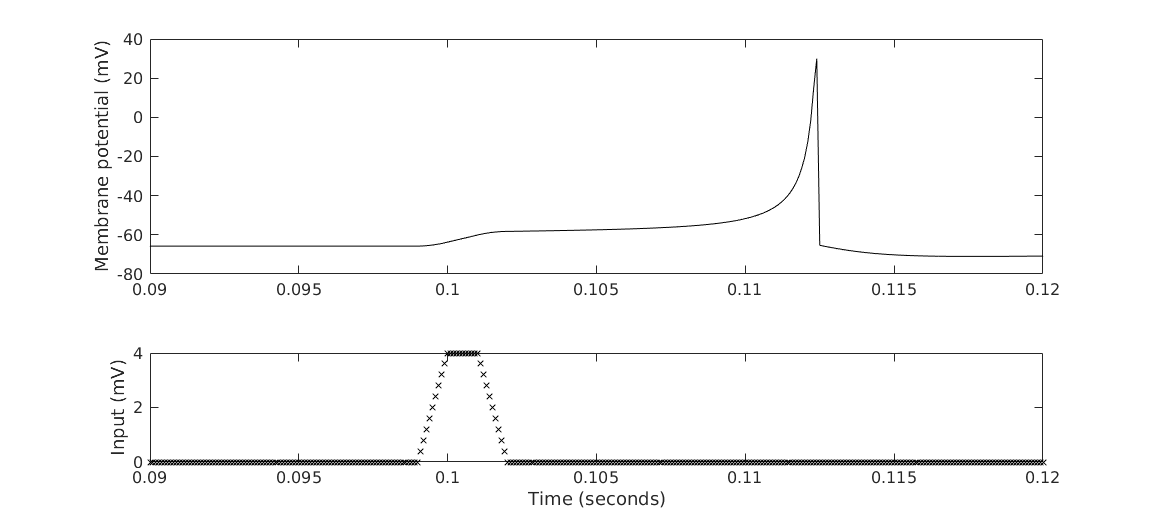
\includegraphics[width=\textwidth]{fig/WaveSpeed_NeuronStepTest}
\end{figure}

To determine  that this spike delay is indeed important to consider  we expose populations of excitatory and inhibitory neurons to current pulses of different magnitudes.
The average firing delay of the excitatory and inhibitory neurons is shown in Figure \ref{fig:delay_neurondynamics}.
The inhibitory neurons have a lower firing threshold than the excitatory neurons due to their higher value of $b$ in Equation \ref{eq:neuron_v}  \citet{izhikevich2003} and fire with a shorter delay when given the same stimulus.
Both excitatory and inhibitory neurons exhibit a delayed response of several $ms$ or more.
\begin{figure}[!htb]
 \caption{ A stronger stimulus creates a spike with less delay. The excitatory neurons have a higher firing threshold than the inhibitory neurons and do not emit a spike for very weak stimulus.}
 \label{fig:delay_neurondynamics}
 \centering
   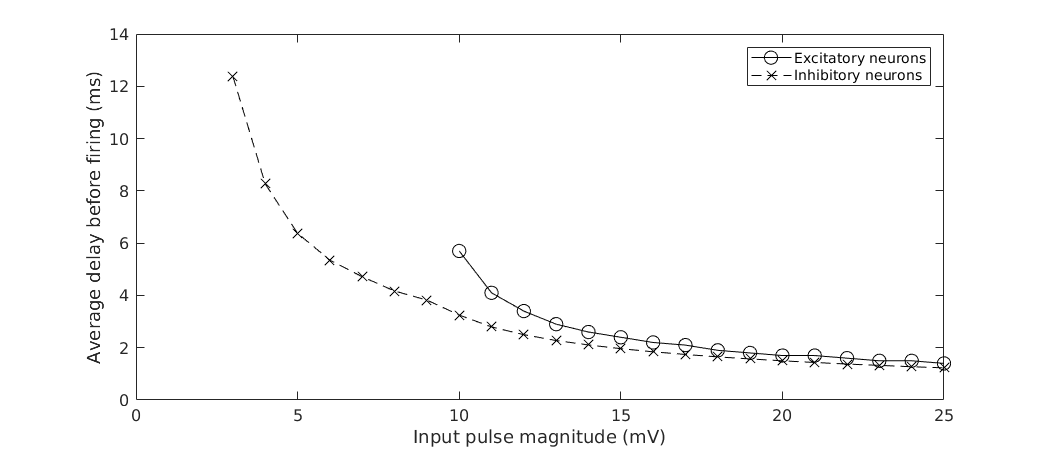
\includegraphics[width=\textwidth]{fig/WaveSpeed_NeuronDynamics}
\end{figure}

\FloatBarrier

To measure wave propagation speed we use an SCE with width 2, height 2, and length 50.
Our exploration of wave speed uses a step stimulus applied to the lowest 10 layers of neurons (see Methods), while no stimulus is applied to the remaining neurons.
We then measure the time for the wave to propagate to the top layer to determine the pace in milliseconds per unit length traveled.
The speed is then calculated as the inverse of the pace in units/millisecond.

We fix the connection normalization constant $C$ in equation \ref{eq:connectivity} to $0.5$ and we fix the stimulus strength $M$ in equation \ref{eq:randomstim} to $5$ and do not vary them.
As mentioned in Methods we use $\Sigma_v$ here, with $K=24$, because the SCE cannot sustain traveling waves at $\Sigma$. 
Here, without the uniform background stimulus the neurons in the SCE are at their equilibrium point when the traveling wave arrives, and it takes a stronger stimulus from the passing wave to elicit a spike.
We increase the connection strength $K$ to provide this stronger stimulus, and find traveling waves that span the SCE starting at $K=18$. 
As $K$ increases the neurons fire with less delay, resulting in faster traveling waves (Figure \ref{fig:delay_k}).
We fix $\Sigma_v = \{K=24,\lambda=2.5,P_{exc}=0.8,\kappa=1.0 \}$ for the remainder of the wave speed computational experiments.

 
We first examine the impact of K on the wave speed.
The wave speed increases with K as anticipated (Figure \ref{fig:delay_k}).
The relationship is logarithmic in shape, in agreement with some previous work including \citet{Golomb1999} (Figure 3 for $\tau_d>0$) and \citet{Golomb1996}(Figure 10, exponential footprint shape).


\begin{figure}[!htb]
 \caption{The pace (left, error bars $\pm 1 \sigma$) decreases with $K$, while the corresponding wave speed (right) increases with $K$. 
          The logarithmic best fit is $0.36\log{0.12K}$.}
 \label{fig:delay_k}
 \centering
   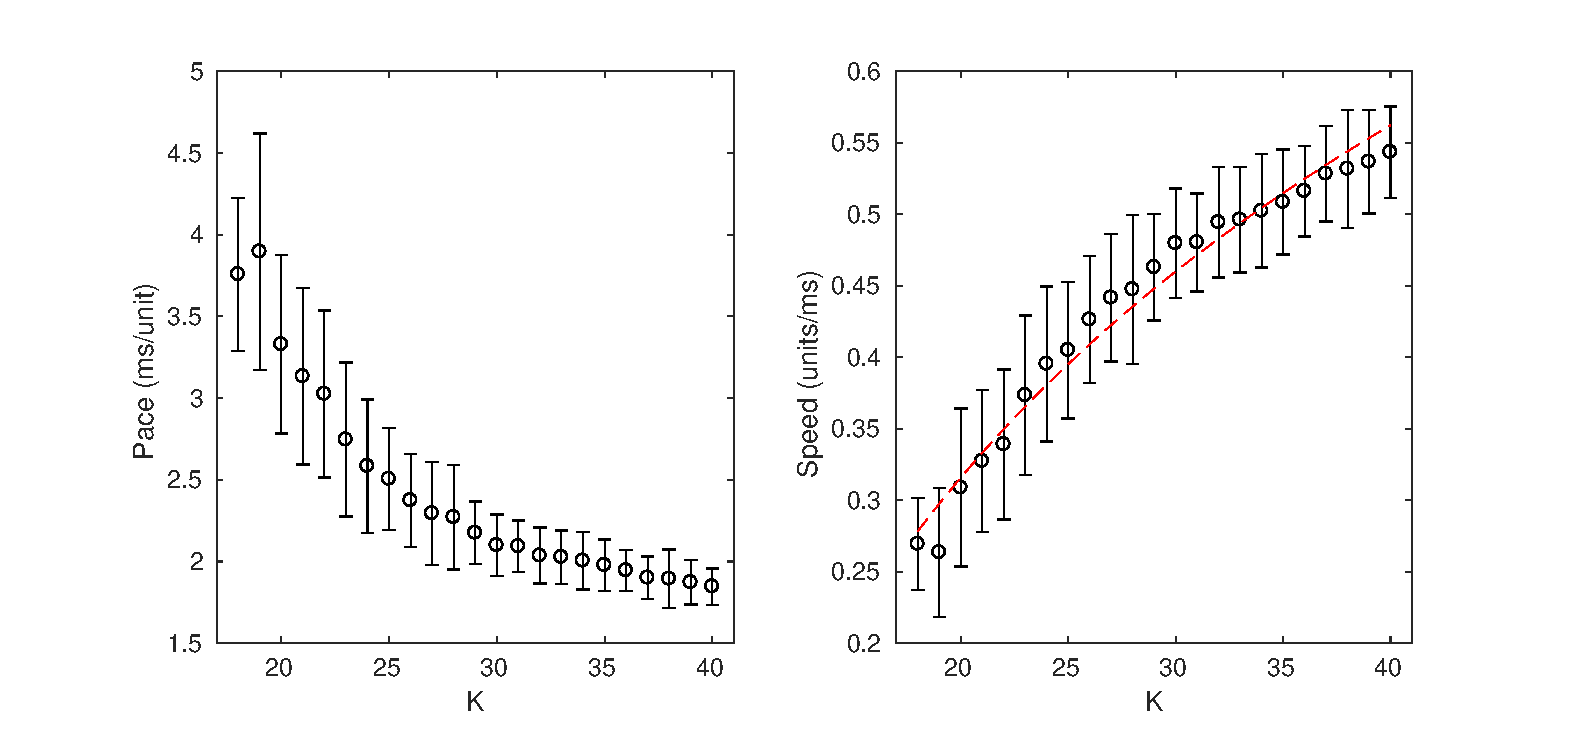
\includegraphics[width=\textwidth]{fig/WaveSpeed_K}
\end{figure}


We examine the influence of the $b$ parameter on wave speed.
We generate $100$ SCE, then multiply the $b$ parameter of all neurons by a scaling factor from $0.7$ to $1.3$.
When the scale factor is $\leq 1.0$ the wave speed remains constant, but when the scale factor is $>1.0$ the wave speed increases linearly (Figure \ref{fig:WaveSpeed_B}).
This indicates that the lower firing thresholds (Figure 6) that result from larger values of the $b$ parameter result in faster traveling waves.

\begin{figure}[!htb]
 \caption{The pace (left, error bars $\pm 1 \sigma$) and the wave speed (right) show a sharp transition above scale factor $1.0$. }
 \label{fig:WaveSpeed_B}
 \centering
   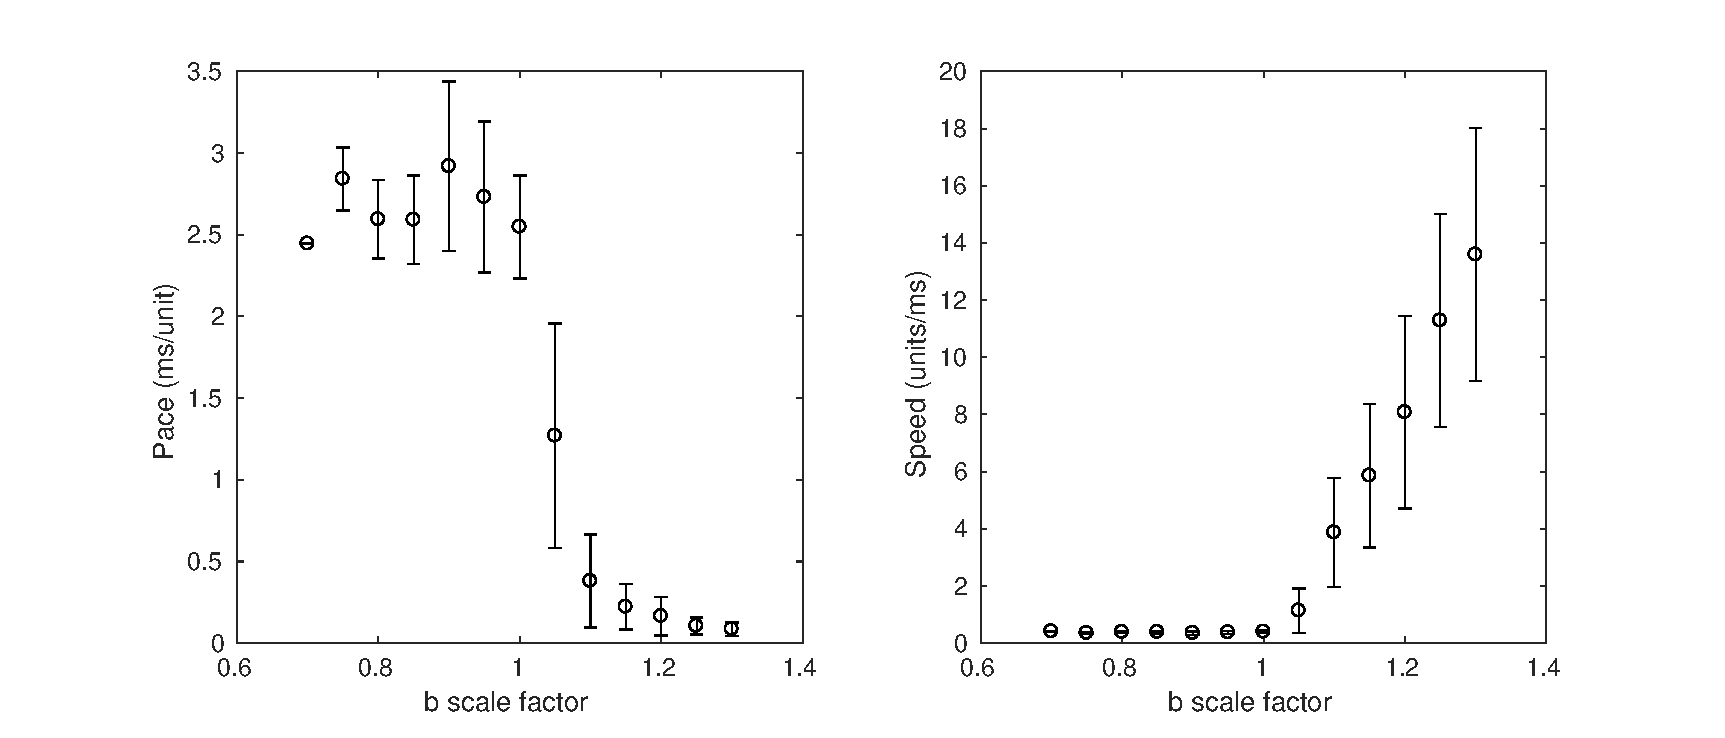
\includegraphics[width=\textwidth]{fig/WaveSpeed_B}
\end{figure}

\FloatBarrier

We next explore the influence of the action potential propagation speed, here controlled by our parameter $\kappa$, on the traveling wave propagation speed.
We vary delay parameter $\kappa$ from 0 to 5 and measure the wave pace and calculate the wave speed (Figure \ref{fig:delay_speed}).
The pace is linear in $\kappa$ as expected, but the pace does not approach $0$ as $\kappa \rightarrow 0$ due to the delayed firing inherent in the neuron dynamics.
Because each neuron does not fire instantaneously upon receiving an action potential, even instantaneous transport of action potentials does not result in a wave that can span the column instantaneously.
\begin{figure}[!htb]
 \caption{The pace (left, error bars $\pm 1 \sigma$) is linear w.r.t. $\kappa$. The intercept at $\kappa=0$ is 1.3, indicating that the neuron dynamics limit the speed of the wave. The wave speed (right) shows the expected relationship. }
 \label{fig:delay_speed}
 \centering
   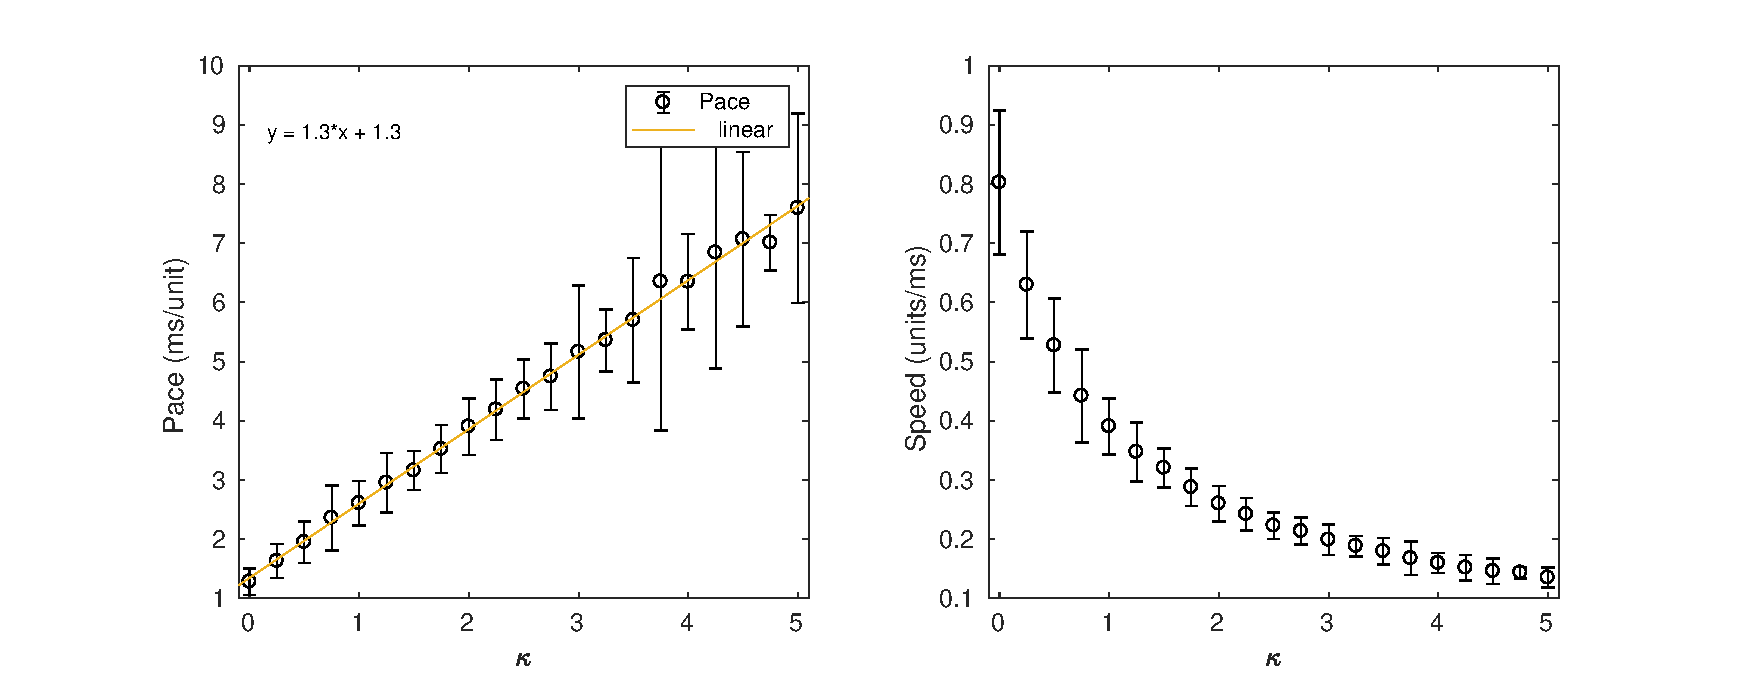
\includegraphics[width=\textwidth]{fig/WaveSpeed_Delay}
\end{figure}
\FloatBarrier

Propagation speed is also influenced by the characteristic length of the local connectivity, $\lambda$.
Since an increase in $\lambda$ results in both longer range connections, and more incoming and outgoing connections per neuron, we expect $\lambda$ to increase the wave speed through both action potential propagation and neuron dynamics.
The characteristic connection length $\lambda$ is varied from 2 to 5 and we measure the wave pace and calculate the wave speed (Figure \ref{fig:delay_lambda}).
For $\lambda<2$  we do not observe traveling waves.
\begin{figure}[!htb]
 \caption{ The pace (left, error bars $\pm 1 \sigma$) decreases with $\lambda$. 
           The wave speed (right) shows that the maximum wave speed approaches $0.8$, the limit seen as $\kappa \rightarrow 0$ in Figure \ref{fig:delay_speed}. 
           The logarithmic best fit to the data is $0.62\log{0.74\lambda}$.}
 \label{fig:delay_lambda}
 \centering
   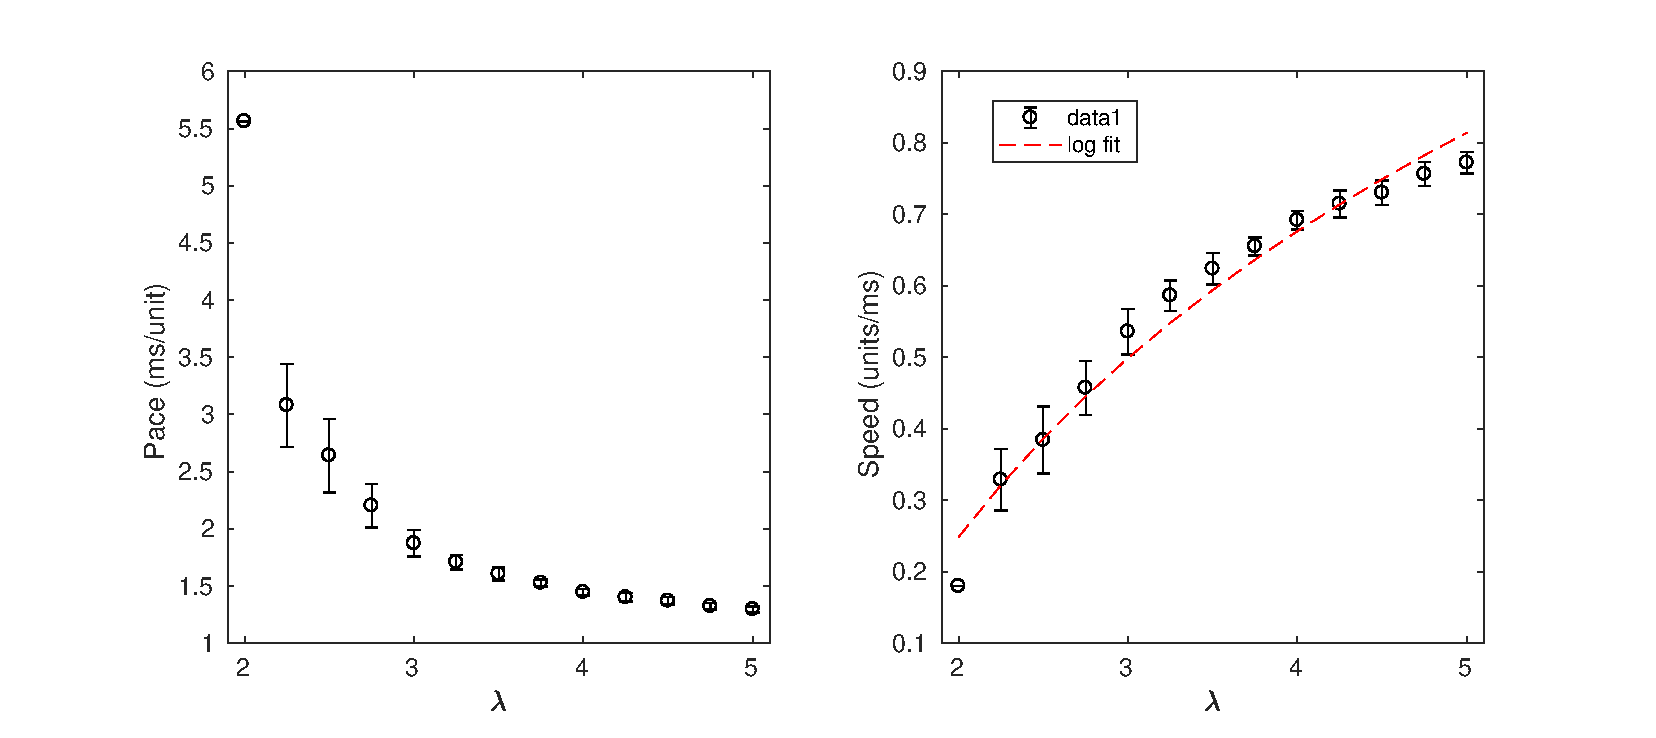
\includegraphics[width=\textwidth]{fig/WaveSpeed_Lambda}
\end{figure}

\FloatBarrier

Our SCE topology (namely, the X and Y dimensions) may influence the wave speed in several ways.
Increasing X and/or Y increases the total number of neurons, the total number of connections, and the average number of connections per neuron.
To test these, we construct columns with topology in XxY of $2x2, 2x3, 3x3, 3x4$ and $4x4$.
We also tested the $1x1$ topology but found that it did not support traveling waves (SI Figure 6).
For each topology we measure the pace and speed over $5$ randomly generated SCE (Figure \ref{fig:delay_topology}).
We see that increasing the X and/or Y dimensions of the SCE increases the speed, and the dependence looks qualitatively similar to increasing the connection strength via $K$ or the number of connections via $\lambda$.

\begin{figure}[!htb]
 \caption{ The pace (left, error bars $\pm 1 \sigma$) decreases, and the speed (right) increases, as the XxY extents of the SCE grow.}
 \label{fig:delay_topology}
 \centering
   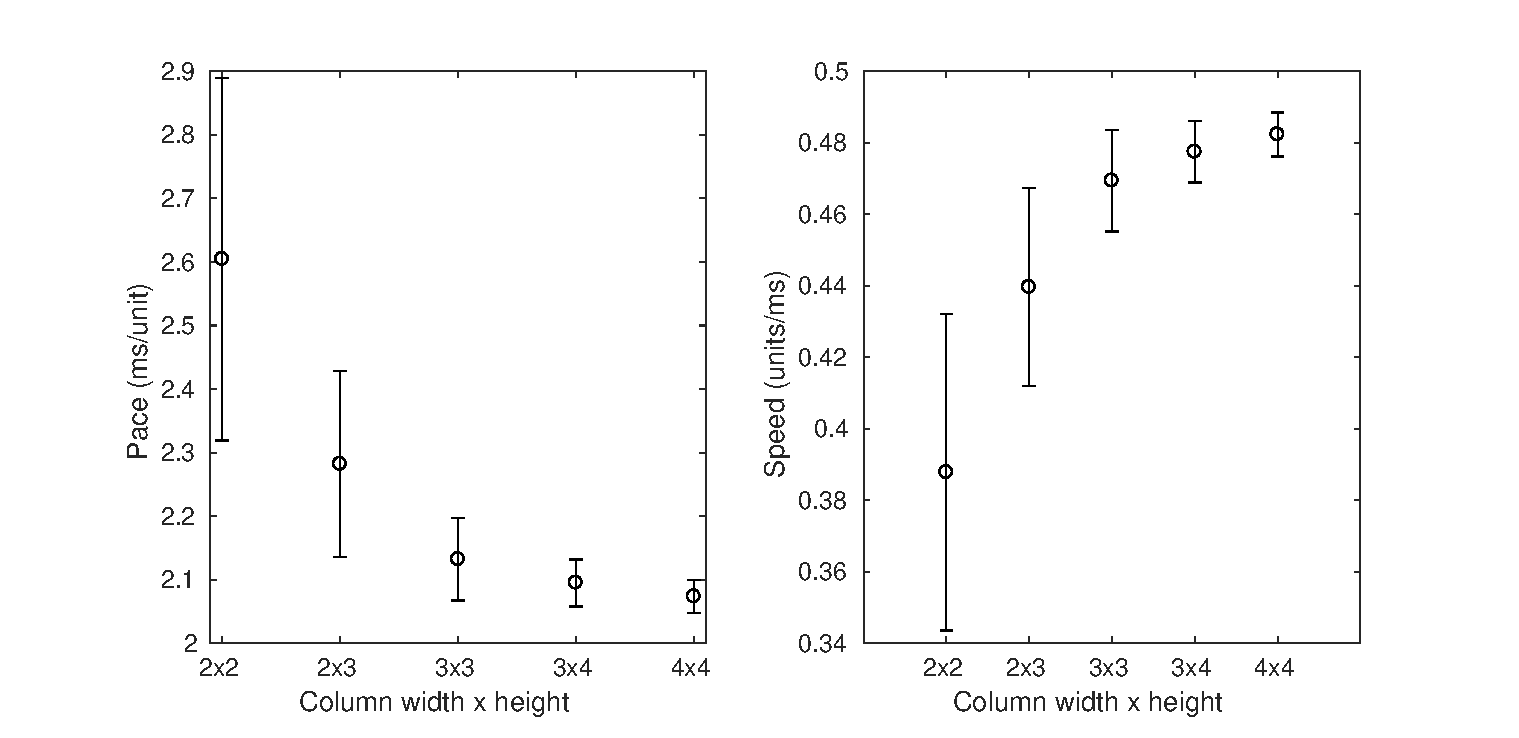
\includegraphics[width=\textwidth]{fig/WaveSpeed_Topology}
\end{figure}

To separate the effect of the increased connectivity from the effect of different topology (larger X or Y increases both the total number of neurons and changes the proportion of surface neurons) we scale the $C$ parameter in equation \ref{eq:connectivity} to maintain the same average number of connections per neuron (\textasciitilde{}7) across the topologies.
Results show that when separated from the increase in connectivity larger cross sections do not change the wave propagation speed (Figure \ref{fig:delay_topology_avgconn}).
Therefore the increase in speed with cross-section seen in Figure \ref{fig:delay_topology} is due entirely to the increasing number of connections per neuron.
Figure 5 in the SI shows additional analysis of SCE with larger cross sections. 

\begin{figure}[!htb]
 \caption{ Wave speed (error bars $1\sigma$) is constant as the topology changes as long as the average number of connections (~7 connections per neuron) is maintained. The largest topology is $13x13$ (169 neurons at base).}
 \label{fig:delay_topology_avgconn}
 \centering
   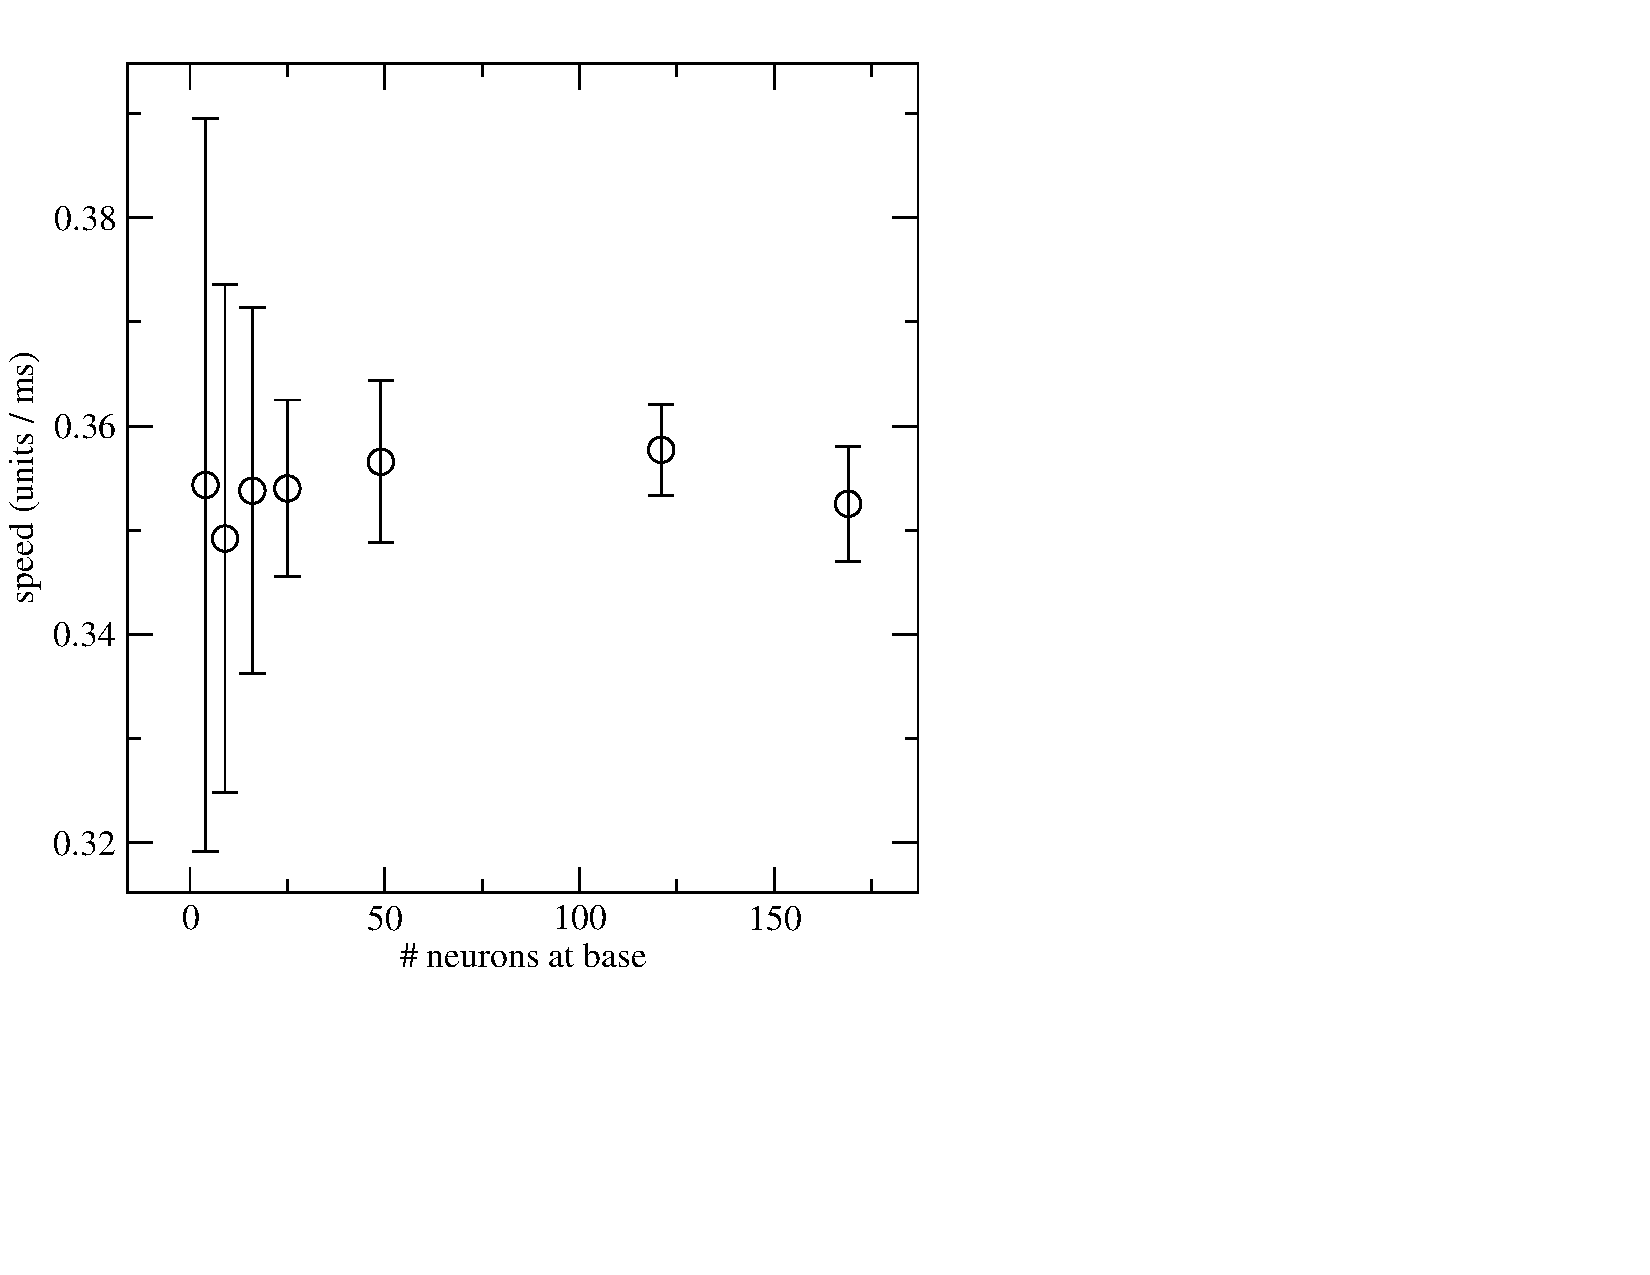
\includegraphics[width=\textwidth]{fig/speed_vs_thick_m}
\end{figure}

\FloatBarrier

It is interesting to compare the speeds obtained here with previous work.
We have placed our neurons on a unit grid and measured speed in units per millisecond.
By assuming that our unit grid is about $20~\mu m$ (Cruz et al., 2005) then our wave propagation speeds are in the range of $2-16~mm/s$.
This is generally slower than other computational results, but the mid to upper range is of the same order of magnitude as the experimental velocity of $50~mm/s$  reported in \citet{Golomb1997}.

\FloatBarrier

\section{Wave Initiation and Density} \label{sub:wave_initiation}
Traveling waves spawned by uniform background stimulation do not appear to originate at random places in the SCE.
Instead we observe that, for a given randomly generated SCE, waves tend to spawn from certain locations within the SCE.
This is most noticeable for SCEs with very dense local connectivity with $C=1.0$ in equation \ref{eq:connectivity}.
To quantify this observation we record the initiation sites of all traveling waves that were observed in an SCE under uniform background stimulus (Figure \ref{fig:wave_initiation_sites}).
We then measure the fraction of wave initiation events (FIE) per unit length of the SCE.

\begin{figure}[!htb]
 \caption{Left: The time and place of origin of every traveling wave produced during a simulation. Right: The FIE clearly shows that traveling waves are likely to start in some regions, and unlikely to start in others.}
 \label{fig:wave_initiation_sites}
 \centering
   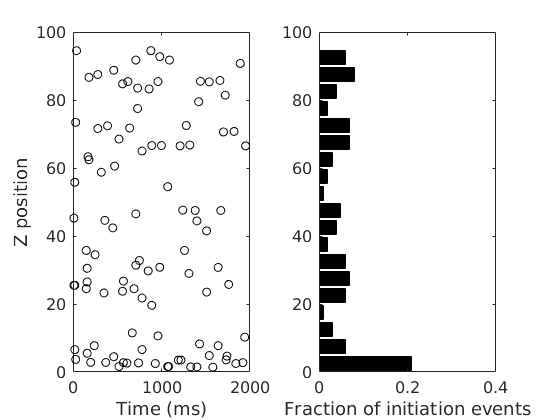
\includegraphics[width=\textwidth]{fig/InitiationSites_100sims}
\end{figure}

A separate observation is that only some of the neurons in the SCE will fire when a wave passes their location.
We observe that a single traveling wave initiated by a step stimulus can have regions of higher or lower total firing activity which we quantify by measuring the fractional number of firing events (FFE) per unit length of the SCE.
An example measurement of the firing activity in a single traveling wave is shown in Figure \ref{fig:wave_density}.
\begin{figure}[!htb]
 \caption{Density of firing events in a traveling wave initiated from a step stimulus. Left: Raster plot of the spike-emission times from a single traveling wave. Right: The FFE shows that some regions of the SCE exhibit more firing activity.}
 \label{fig:wave_density}
 \centering
   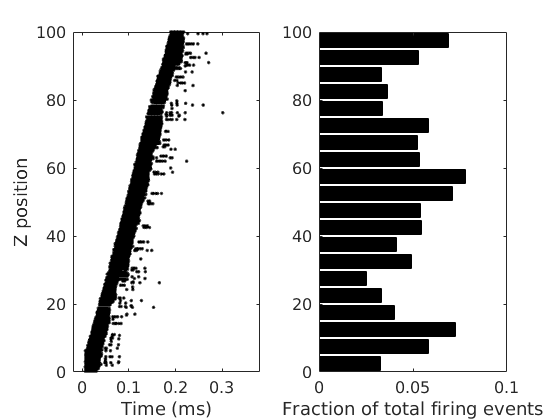
\includegraphics[width=\textwidth]{fig/ImpulseWaveDensity}
\end{figure}

By combining these two experiments we observe that the results from the FIE and the FFE appear anti-correlated. 
In Figure \ref{fig:fie_ffe_plots} we see multiple FIE and FFE plots from the same SCE placed side-by-side.
There is a visual anti-correlation between the FIE and FFE for each SCE although it is not conclusive from these plots.
\begin{figure}[!htb]
 \caption{FIE and FFE for nine example columns. } 
 \begin{tabular}{ccc}
     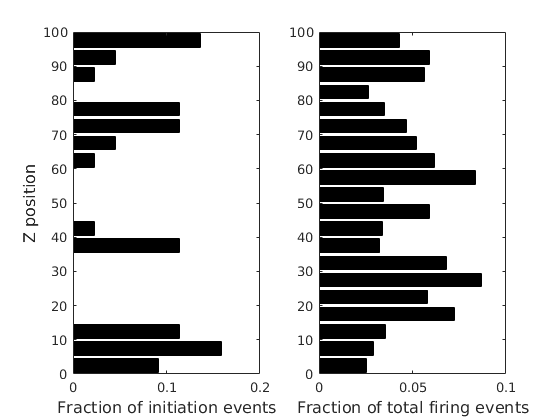
\includegraphics[width=0.3\textwidth]{fig/ccf/ccf1} & 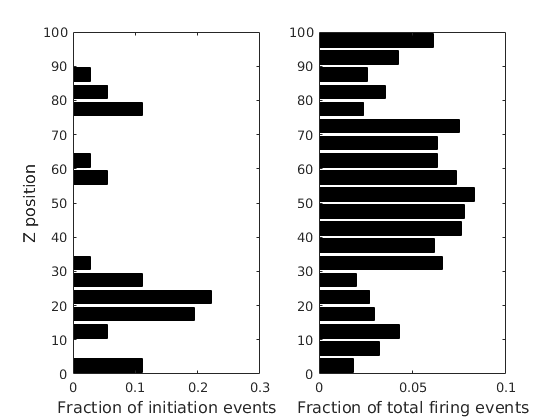
\includegraphics[width=0.3\textwidth]{fig/ccf/ccf2} & 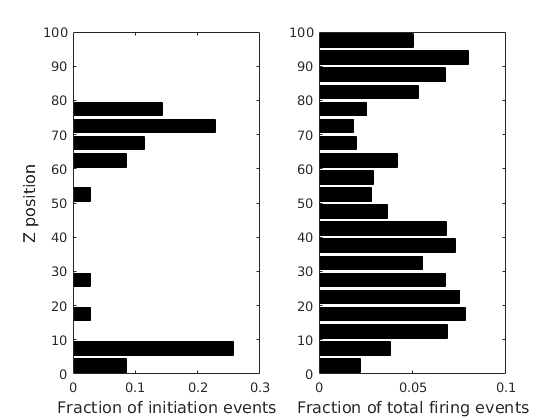
\includegraphics[width=0.3\textwidth]{fig/ccf/ccf3} \\
     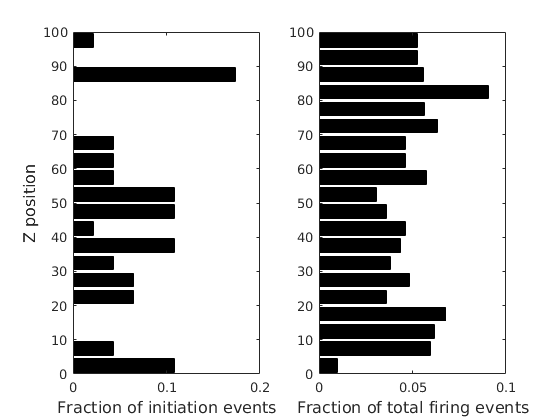
\includegraphics[width=0.3\textwidth]{fig/ccf/ccf4} & 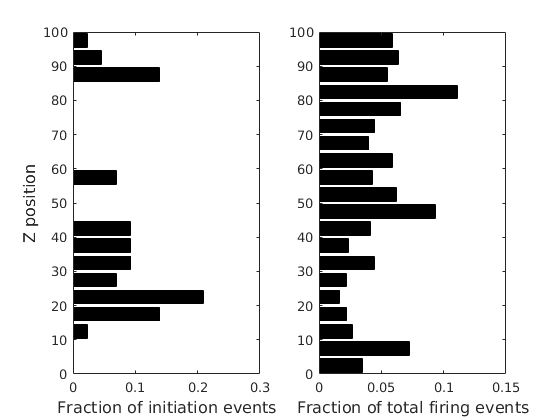
\includegraphics[width=0.3\textwidth]{fig/ccf/ccf5} & 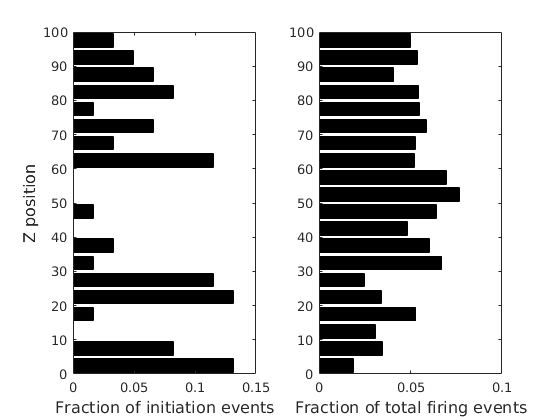
\includegraphics[width=0.3\textwidth]{fig/ccf/ccf6} \\
     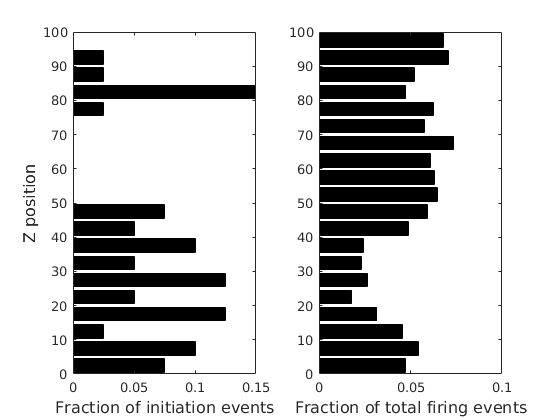
\includegraphics[width=0.3\textwidth]{fig/ccf/ccf7} & 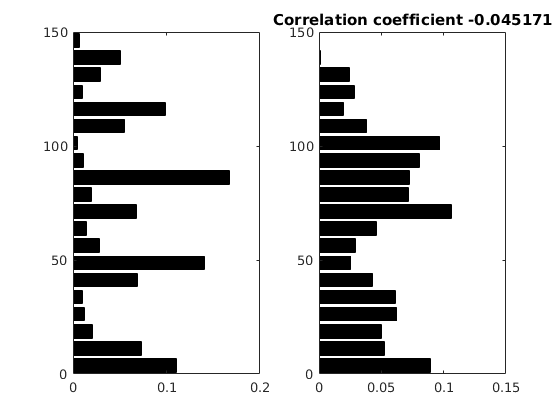
\includegraphics[width=0.3\textwidth]{fig/ccf/ccf8} & 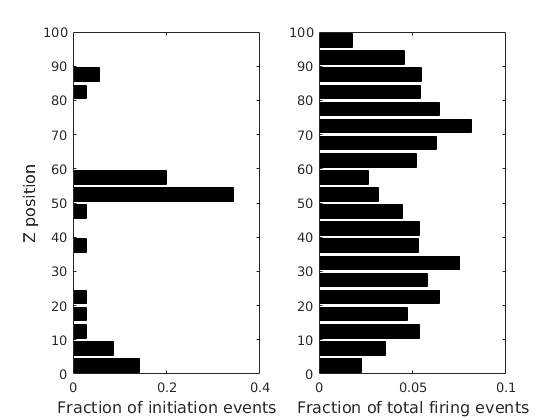
\includegraphics[width=0.3\textwidth]{fig/ccf/ccf9} 
 \end{tabular}
 \label{fig:fie_ffe_plots}
\end{figure}

\FloatBarrier

To test that this observation is generally true we create 100 SCEs, apply first uniform background stimulus and then step stimulus to each SCE, and measure the correlation between the FIE and FFE (Figure \ref{fig:InitiationCorrelation}).
The correlation coefficient is estimated from the two histograms using MATLAB 'corrcoef'.  
Although there is substantial variation between SCEs we measure a consistently negative correlation coefficient (mean $-0.26$, standard deviation $0.18$) between FIE and FFE results.
A one-sided t-test at the $1\%$ confidence level rejects the null hypothesis that the mean of the correlation coefficient is $0$ or greater.
\begin{figure}[!htb]
 \centering
 \caption{ A) Correlation between FIE and FFE across 100 trials. B) Distribution of the correlation coefficient. Each trial is a new SCE with random neuron and connectivity parameters. }
 \label{fig:InitiationCorrelation}
 \begin{tabular}{c}
     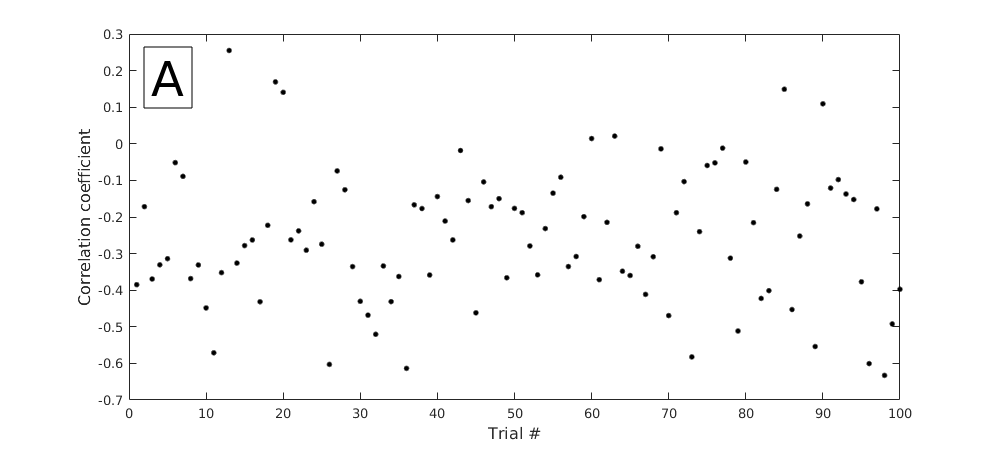
\includegraphics[width=\textwidth]{fig/InitiationCorrelation} \\ 
     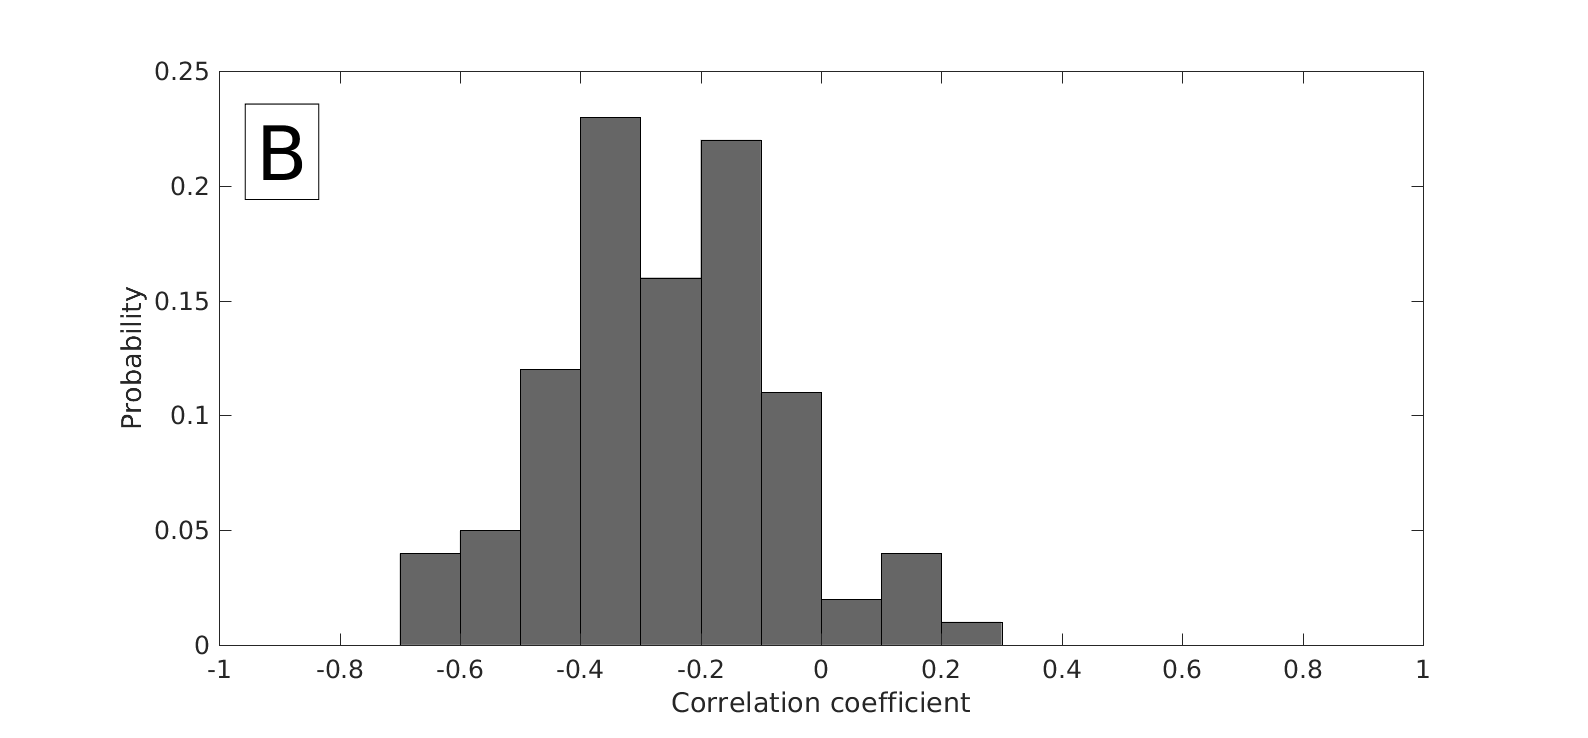
\includegraphics[width=\textwidth]{fig/InitiationCorrelationPDF} 
 \end{tabular}
\end{figure}

We hypothesize that these preferential wave initiation sites are created by neurons with low firing thresholds that are easy to excite.
In the Izhikevich model, inhibitory neurons can have a lower firing threshold than excitatory neurons, modeling the behavior of real inhibitory neurons in the cortex\citet{gibson2009}\citet{hayut2011}.
As we can see from figure \ref{fig:delay_neurondynamics}  the $b$ parameter in the Izhikevich model sets the firing threshold of the individual neurons.
Neurons with higher $b$ parameter are easier to excite and therefore more likely to fire.
Per Table \ref{tab:izzy_params} excitatory neurons all have a $b$ parameter of $0.2$, while inhibitory neurons have $b$ parameters in the range $0.2-0.25$.
This indicates the preferential wave initiation sites could be due to low-threshold spiking (LTS) inhibitory neurons \citet{izhikevich2003}.
It may seem counter-intuitive that firing activity from an \underline{inhibitory} neuron would generate traveling waves.
In fact, postinhibitory rebound spiking is observed in both cortical neurons \citet{ascoli2010} and the Izhikevich model of neuron dynamics,  and was studied in the context of spindle waves in the thalamus in \citet{Golomb1996}.
The LTS hypothesis also explains the reduced wave density at these sites.
As a traveling wave passes through the region, because of their increased activity these same inhibitory neurons suppress the surrounding neurons resulting in fewer local firing events.

A comparative computational experiment shows that low-threshold spiking inhibitory neurons can indeed generate traveling waves under background stimulus.
We first create an SCE with entirely excitatory neurons.
We then create an identical SCE except for a single LTS inhibitory neuron at $Z=50$.
The $b$ parameter of the LTS inhibitory neuron is set to $0.25$, corresponding to the lowest firing threshold used in our model.
These two SCEs are stimulated with the same uniform background stimulus. 
Figure \ref{fig:lts_inhibit} clearly shows that adding the single LTS neuron results in traveling waves emanating from $Z=50$. 
\begin{figure}[!htb]
 \caption{Simulation with a single LTS inhibitory neuron at $Z=50$. Left: an SCE with entirely excitatory neurons shows traveling waves emerging from various locations. Right: adding a single LTS neuron at $Z=50$ results in consistent wave generation from that location. }
 \label{fig:lts_inhibit}
 \centering
   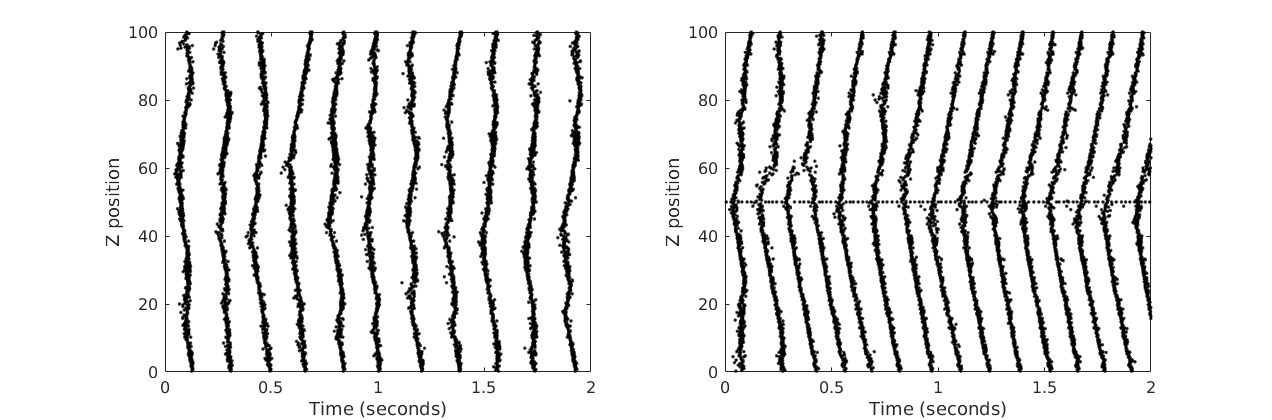
\includegraphics[width=\textwidth]{fig/SingleLTSInhibit}
\end{figure}

\FloatBarrier

\subsection{Wave patterns in fully connected networks} \label{sub:delay}
Our investigation has been concerned with traveling waves of activations that spread through locally connected networks.
We now examine whether traveling wave patterns can also be observed in fully connected networks.
We show that this is possible provided we consider the action potential propagation delay proportional to the distance between neurons, as used in all the simulations above.
We simulate an SCE with complete connectivity corresponding to $\lambda \rightarrow \infty$: all neurons are connected with probability 1 to all other neurons.
This is analogous to the original Izhikevich simulation \citet{izhikevich2003} that demonstrated synchronized firing in a completely connected neural field with random background stimulus.
We first simulate the SCE with a fixed action potential propagation delay of $1.7~ms$ \citet{Markram1997}  regardless of inter-neuron distance.
The result is highly synchronized simultaneous firing among all neurons in the SCE.
 
With distance-dependent propagation delays and fast spike propagation ($\kappa=0.1$) we observe similar synchronized firing.
We then increase $\kappa$ and observe the emergence of traveling wave patterns (Figure \ref{fig:delay_waves}). 
This demonstrates that one dimensional traveling waves can emerge from fully-connected networks if the propagation delay is proportional to the inter-neuron distance and the spike propagation time is above a critical value.
\begin{figure}[!htb]
 \caption{With global connectivity and action potential propagation delay fixed at $1.7~ms$ , the entire structure shows synchronized firing events.
          With distance-dependent propagation we also observe synchronized firing at $\kappa=0.1$.
          As $\kappa$ increases traveling waves emerge ($\kappa=0.5, 1.0$) .}
 \centering
   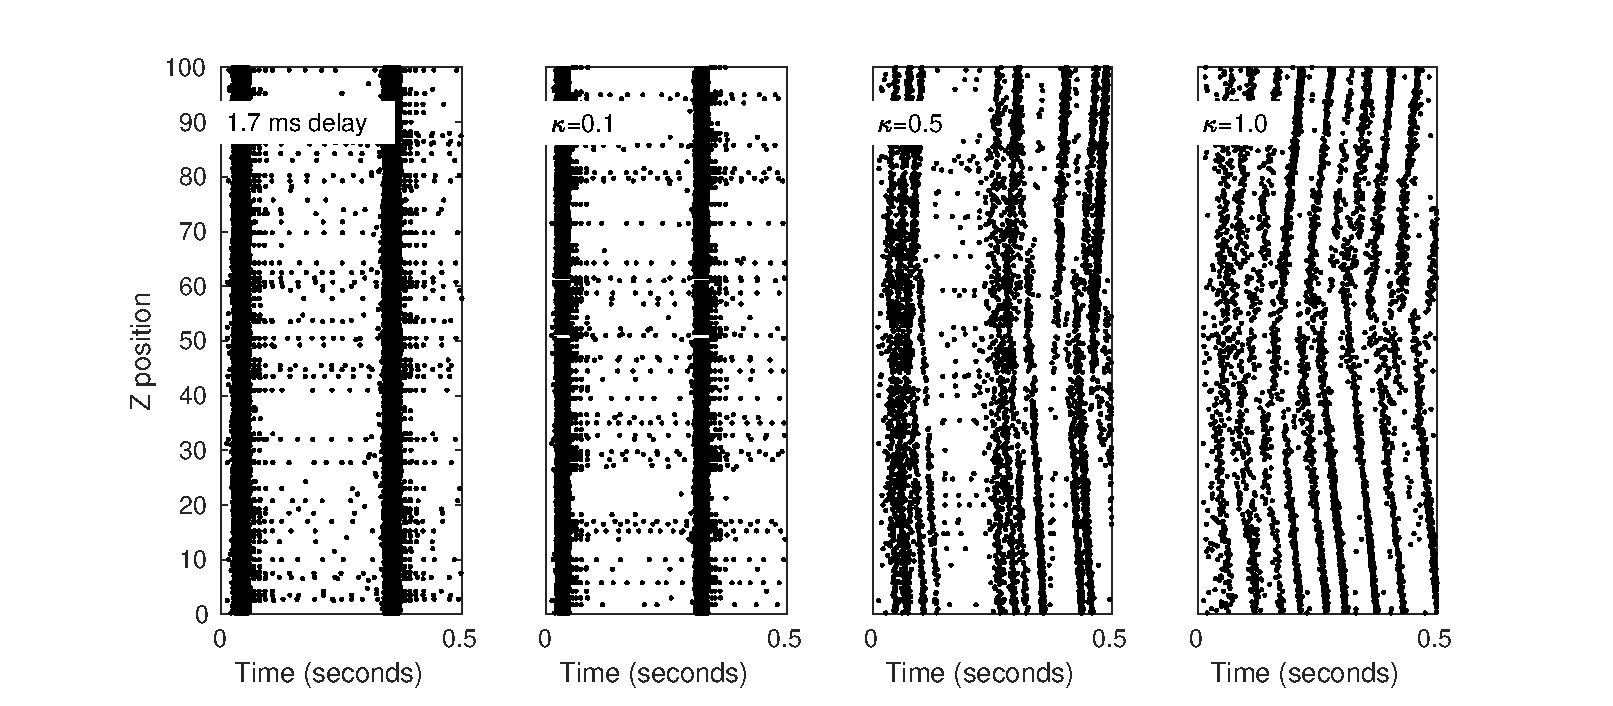
\includegraphics[width=\textwidth]{fig/DelayWaves}  
 \label{fig:delay_waves}
\end{figure}

The present case is similar to previous work that considered coupled oscillators  (\citet{ermentrout2001}, Figure 1) that proposed several models for traveling waves in the cortex.
The one most relevant to traveling waves in our fully-connected networks is a driving source at a spatial location that produces traveling wave patterns due to the propagation delay of action potentials.
This is a fundamentally different type of traveling wave than a chain of spike events that spreads to neighboring neurons due to local connectivity.

\endinput
%%
%% End of file `example-1.tex'.

%%
%% This is file `example-1.tex',
%% generated with the docstrip utility.
%%
%% The original source files were:
%%
%% drexel-thesis.dtx  (with options: `example-part')
%% 
%% This is a generated file.
%% 
%% Copyright (C) 2010 W. Trevor King
%% 
%% This file may be distributed and/or modified under the conditions of
%% the LaTeX Project Public License, either version 1.3 of this license
%% or (at your option) any later version.  The latest version of this
%% license is in:
%% 
%%    http://www.latex-project.org/lppl.txt
%% 
%% and version 1.3 or later is part of all distributions of LaTeX version
%% 2003/06/01 or later.
%% 

\chapter{Quasi 2-D and 2.5-D Systems}
Studies of traveling waves have focused on two-dimensional waves that spread parallel to the surface (pia) of the brain \citep{reimer2010}\citep{keane2015}\citep{Townsend2018}\citep{Golomb1997}\citep{Qi2015}. 
This is to be expected as this is the geometry of the system on which they are observed, and \citep{Wilson1973} provide an anatomical argument for focusing on such structure. 

We now extend our study of traveling waves in quasi 1-D minicolumns to two-dimensional topologies.
First we study two-dimensional sheets of neurons extended in the X and Y directions.
As before, we find that our model doesn't support traveling waves in a purely two-dimensional sheet (Z=1) under the model parameters studied.
When we extend the system to a quasi two-dimensional sheet (Z=2) we find traveling waves are evoked by both the background and impulsive stimulus.

We then further extend our topology to what we term a ``forest'' of minicolumns.
This structure consists of an ensemble of our minicolumns arranged on a grid, with the Z extent less than the X/Y extents.
We find that our forest supports trasverse traveling waves in the X/Y plane.

\section{Two-dimensional sheets of neurons}
Traveling waves in two-dimensional neuronal sheets have been studied in the brain \citep{huang2004}\citep{Townsend2018} and in simulation\citep{keane2015}\citep{Spreizer2019}
While one-dimensional waves have only one structure, the additional degree of freedom in two dimensions allows for several categories of waves.
These include circular waves that spread outward from a point, large plane waves that propagate over the entire surface and spiral waves that rotate around a phase singularity.
We find evidence for all these categories of waves in our quasi two-dimensional sheet.

Each sheet consists of neurons placed on a unit grid. 
The X and Y extents are much larger than the Z extent.
We generally use sheets with Z=2 with the exception of one purely two-dimensional example with Z=1.
Neurons are created and connected as described in Methods.
Due to the larger area of regard and the more demanding computational experiments we use periodic boundary conditions in our quasi two-dimensional sheets.
A small example quasi 2-D sheet is shown in Figure \ref{fig:sheet_structure}.
In this small example the periodic boundary conditions are easily seen in the connection matrix.

\begin{figure}[!htb]
 \caption{Example small quasi 2-D sheet with dimensions X=20, Y=20, Z=2, $\lambda$=2.5, and C=0.5. 
 a)  Sheet showing connections between neurons as lines colored using a color scale that indicates the connection length. 
 b)  Connection matrix. E-E connections are green, E-I are black and both I-E and I-I  are red. 
 c) The sum of presynaptic weights for each neuron shows the anisotropy of this model, with substantial variation in input strength and sign between the neuron inputs.}
 \label{fig:sheet_structure}
 \subfloat[][]{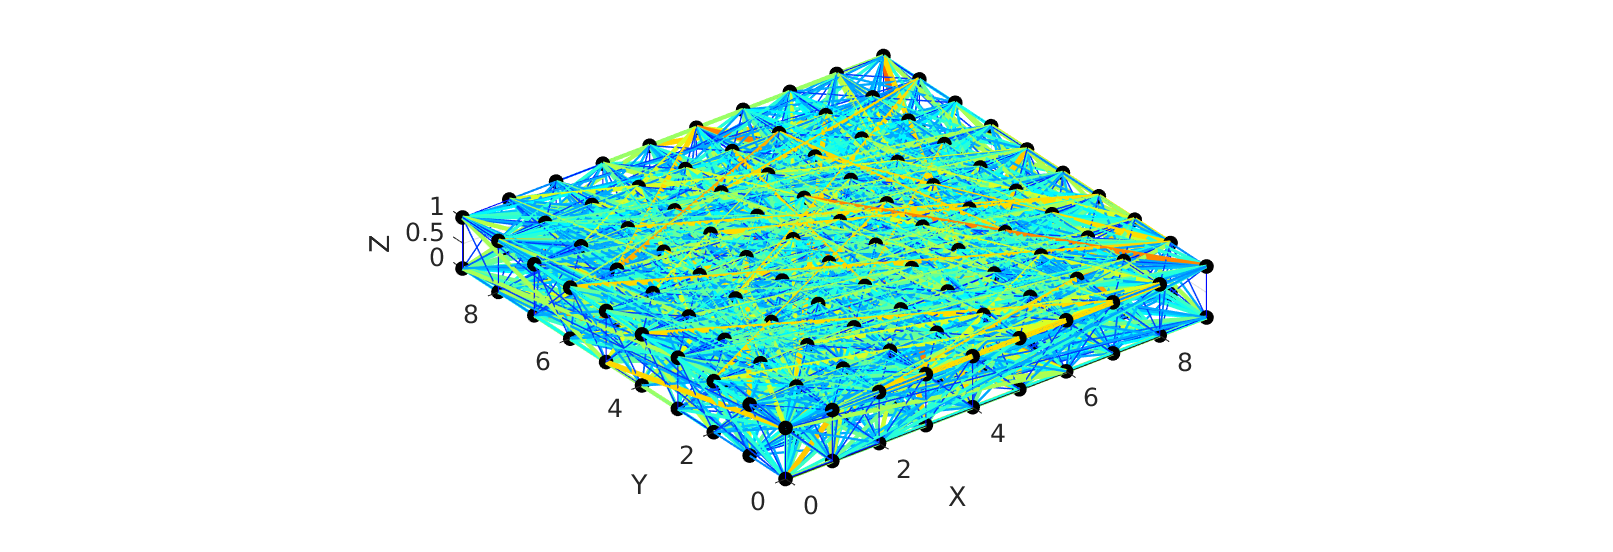
\includegraphics[width=\textwidth]{fig/Sheet_Structure_A}}
 \subfloat[][]{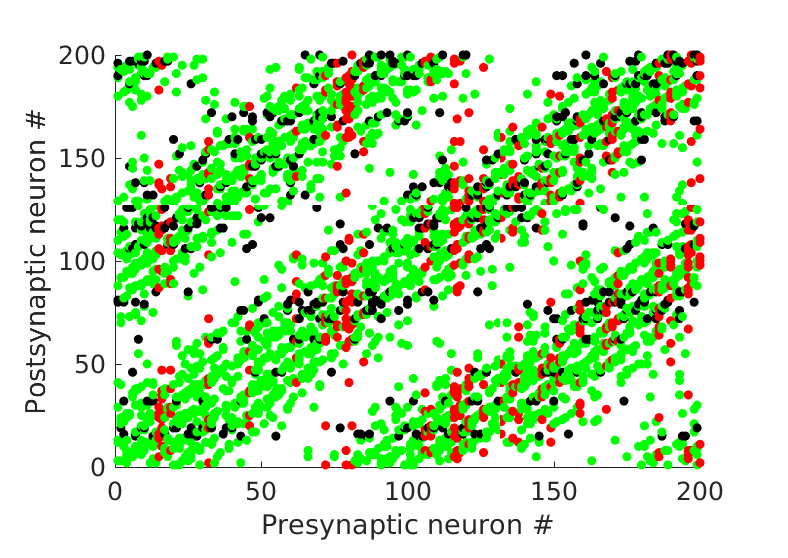
\includegraphics[width=0.4\textwidth]{fig/Sheet_Structure_B}}
 \subfloat[][]{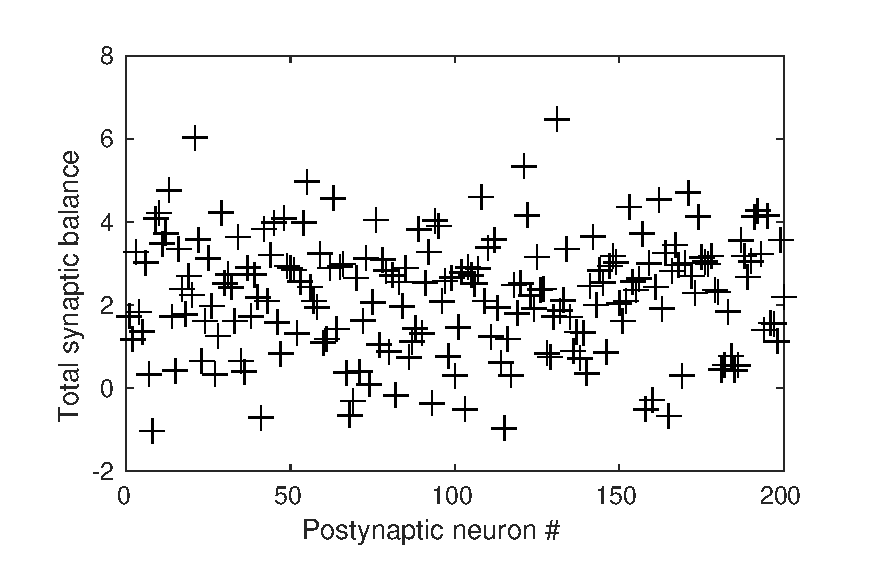
\includegraphics[width=0.4\textwidth]{fig/Sheet_Structure_C}}
\end{figure}

The topology of our sheet combined with our local connectivity rule (eq. \ref{eq:connectivity}) defines the connection distribution of the sheet.
The distribution of post-synaptic connections and delay times are shown in Figure \ref{fig:connection_delay_distrbution_2D} for an example quasi 2-D sheet.
Compared the to minicolumn connection distribution in figure \ref{fig:connection_delay_distrbution} the neurons in our sheet have on average about twice as many connections.
The length of the connections between neurons tends to be longer in the sheet, resulting in a distribution of longer delays 
in figure \ref{fig:connection_delay_distrbution_2D} when compared to figure \ref{fig:connection_delay_distrbution}.
\begin{figure}[!htb]
 \caption{Distribution of (a) number of post-synaptic connections per neuron and (b) delay time. 
          Data was taken from a X=100, Y=100, Z=2 sheet with $\lambda=2.5$, $\kappa=1$ and periodic boundary conditions.  } 
     \subfloat[][]{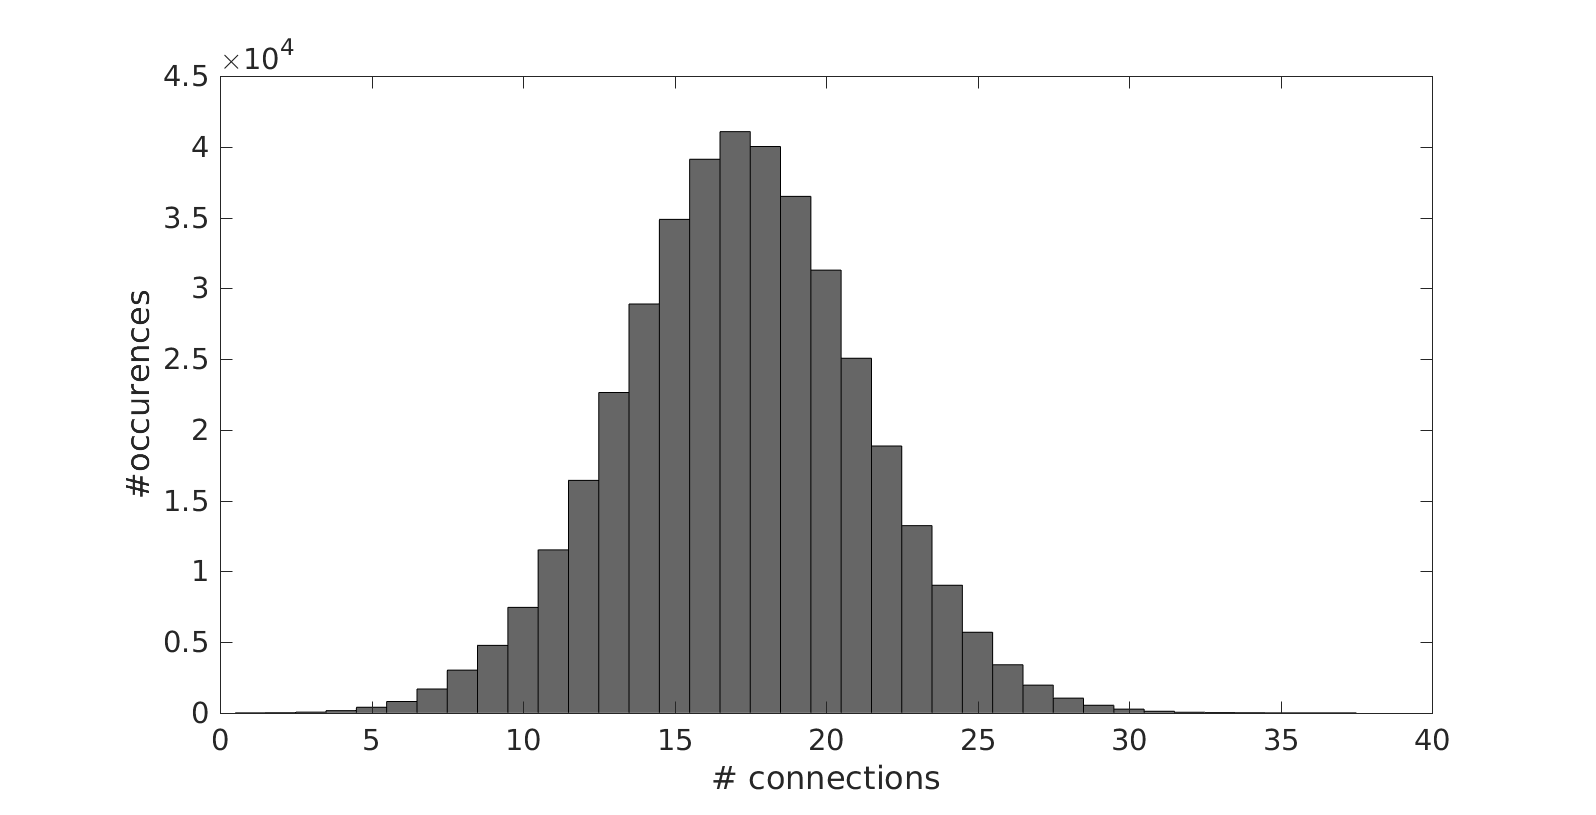
\includegraphics[width=0.6\textwidth]{fig/ConnectionNumberDistribution2D} }
     \subfloat[][]{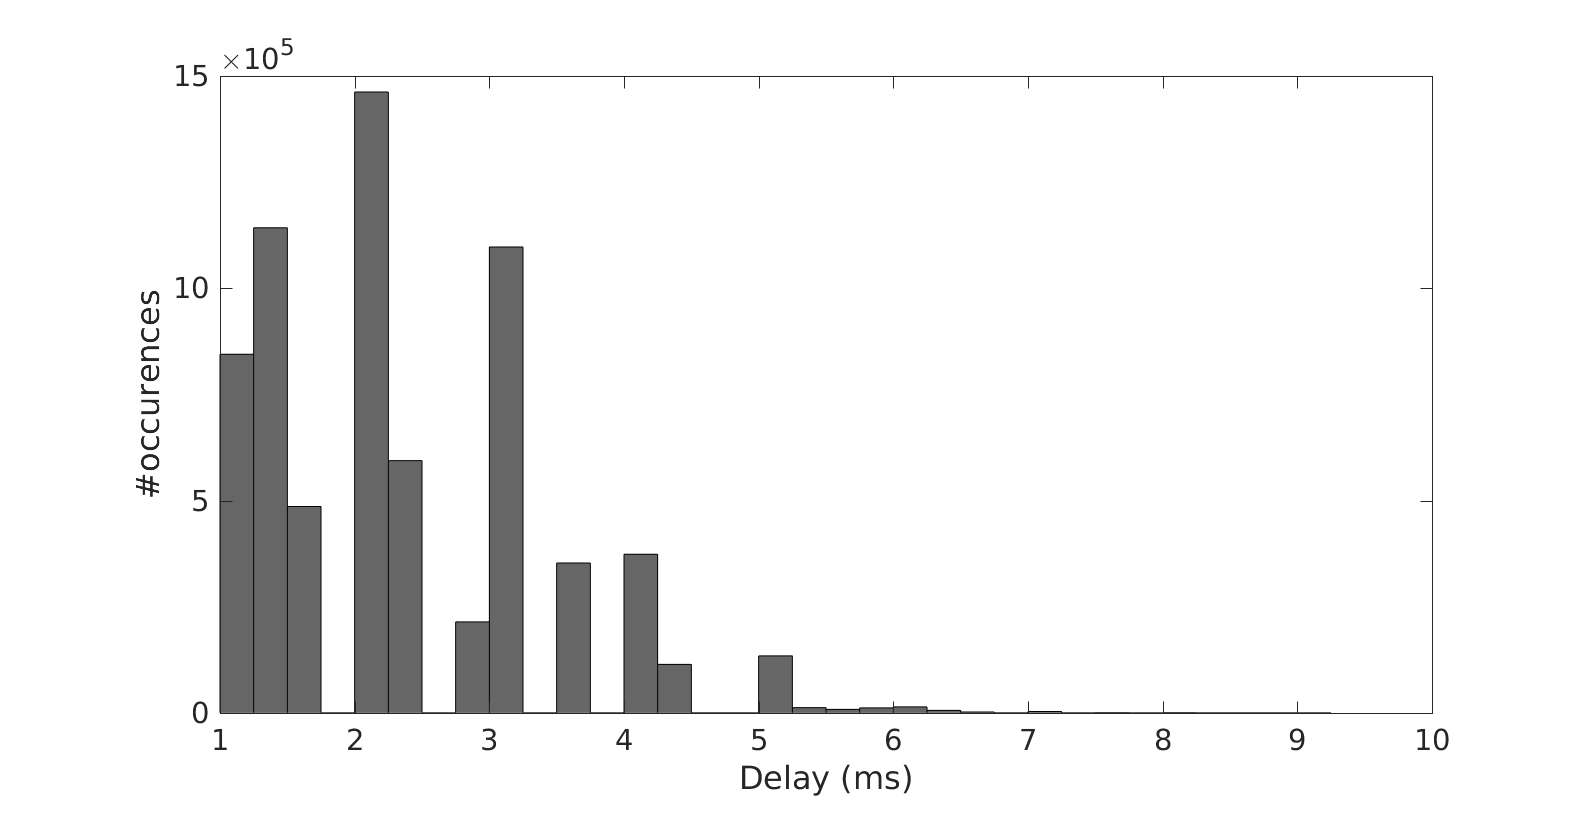
\includegraphics[width=0.6\textwidth]{fig/DelayDistribution2D} }
 \label{fig:connection_delay_distrbution_2D}
\end{figure}
 \FloatBarrier

As we did with our quasi 1-D minicolumn, we first create a purely 2-D sheet of neurons with X=100, Y=100 and Z=1.
Model parameters are fixed at $\Sigma$.
We do not observe traveling waves or other spatiotemporal patterns in this system (Figure \ref{fig:Pure2DRasters_NoWaves}).
\begin{figure}[!htb]
 \caption{ Raster plots from our purely 2-D system do not show coherent spatiotemporal patterns.}
 \label{fig:Pure2DRasters_NoWaves}
 \centering
   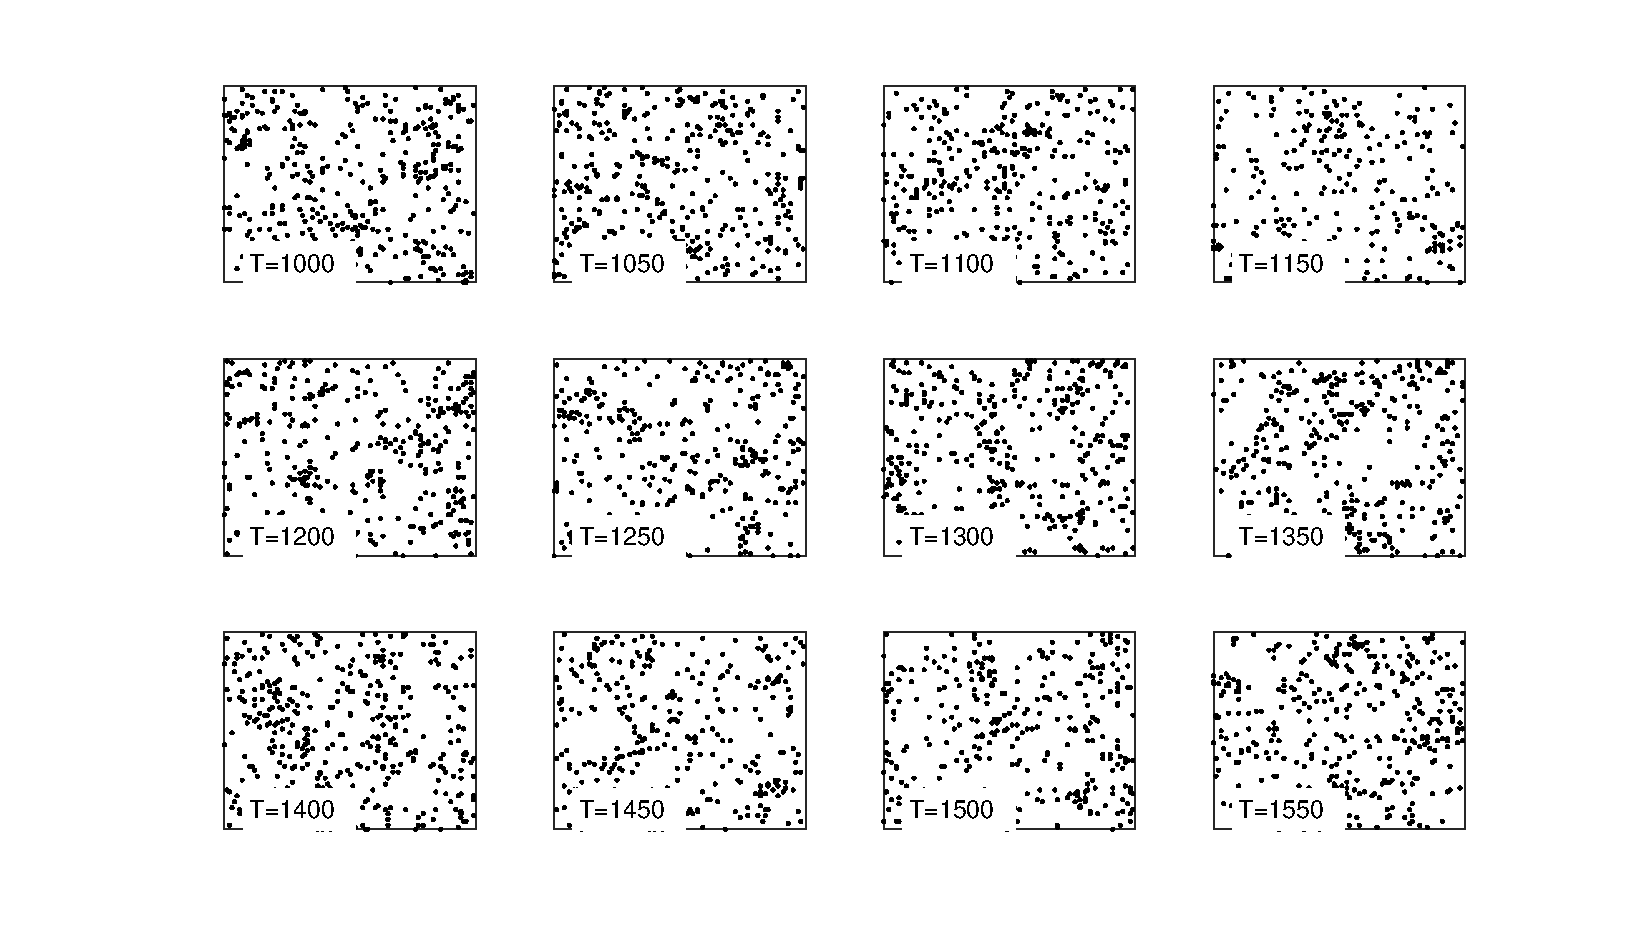
\includegraphics[width=\textwidth]{fig/2DWaveRasters_1LayerNoWaves}
\end{figure}
\FloatBarrier

We then extend our system to a quasi 2-D sheet with X=100, Y=100 and Z=2.
We now observe traveling wave patterns in the system.
These patterns emerge in spite of the high variability in the neuron types, neuron dynamics and connectivity present in our model.
We can clearly see an example of a circular spreading wave emanating from the upper center of figure \ref{fig:2D_waves}.
\begin{figure}[!htb]
 \caption{ Raster plots from our quasi 2-D system with two layers show wave patterns that spread across the surface of the sheet.}
 \label{fig:2D_waves}
 \centering
   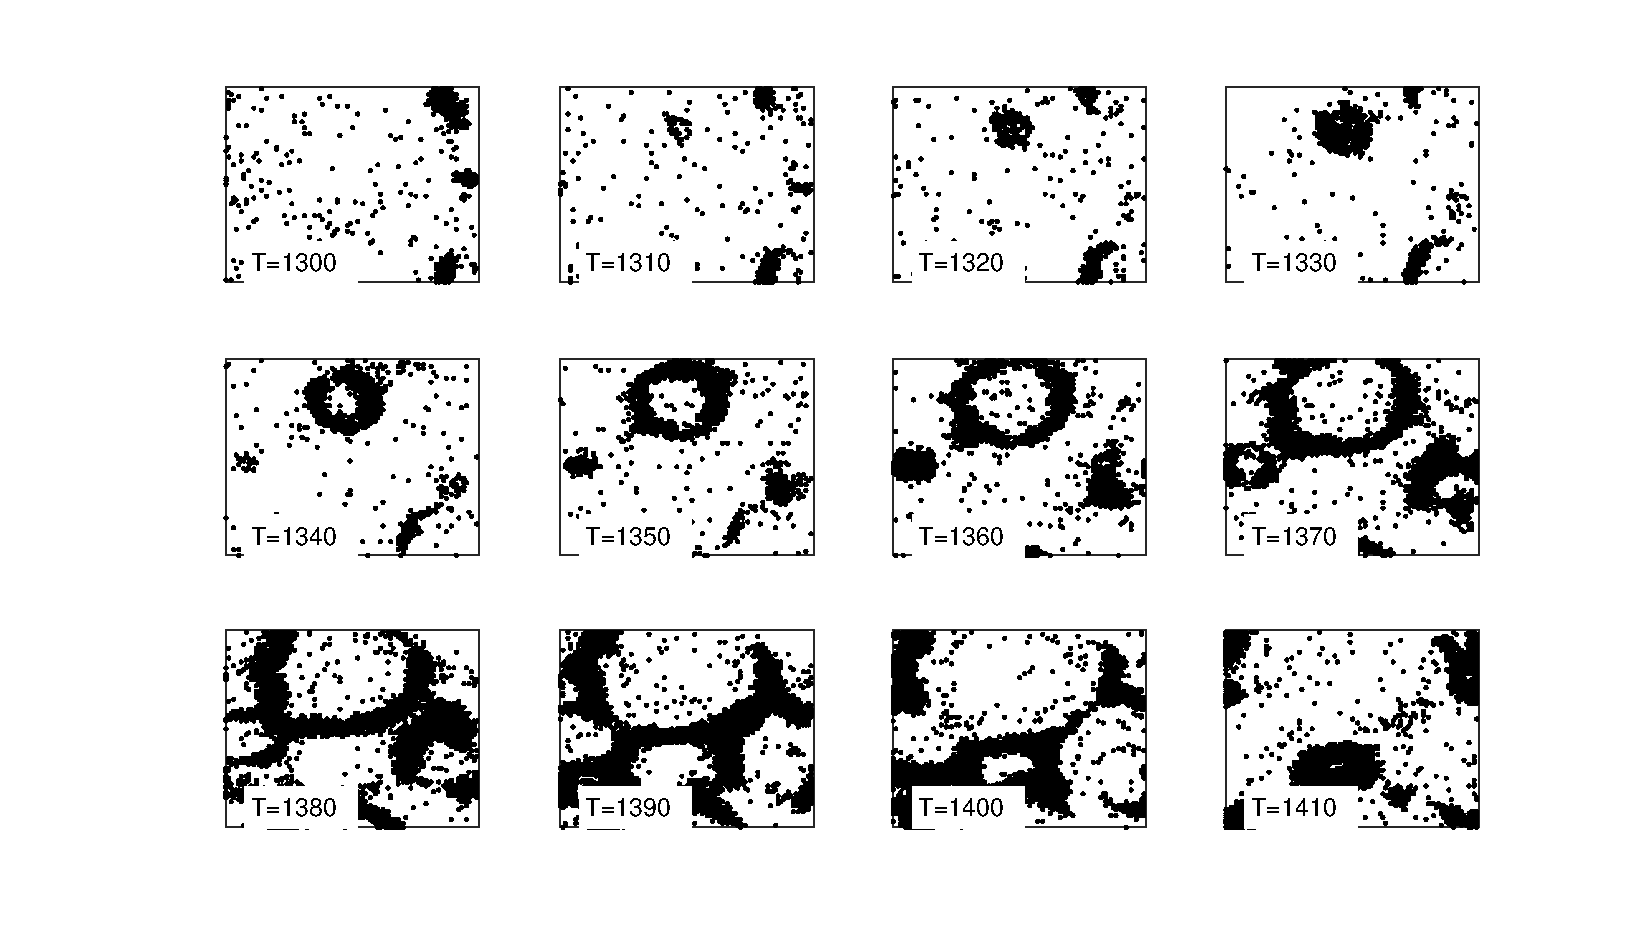
\includegraphics[width=\textwidth]{fig/2DWaveRasters}
\end{figure}

In some simulations we see the formation of large-scale plane waves across the entire system as seen by \citet{keane2015}.
In their work, plane waves were formed when excitation dominated their neuronal system.
The formation of these plane waves in our system does not seem deterministic, as a different random draw of the uniform background stimulus for the same neuronal system may not exhibit plane waves.
Nonetheless, these results show that plane waves can emerge as a stable pattern in systems of this type even when excitation does not dominate.
\begin{figure}[!htb]
 \caption{ Raster plots from our quasi 2.5-D system showing large-scale plane waves moving from top to bottom.}
 \label{fig:2D_plane_wave}
 \centering
   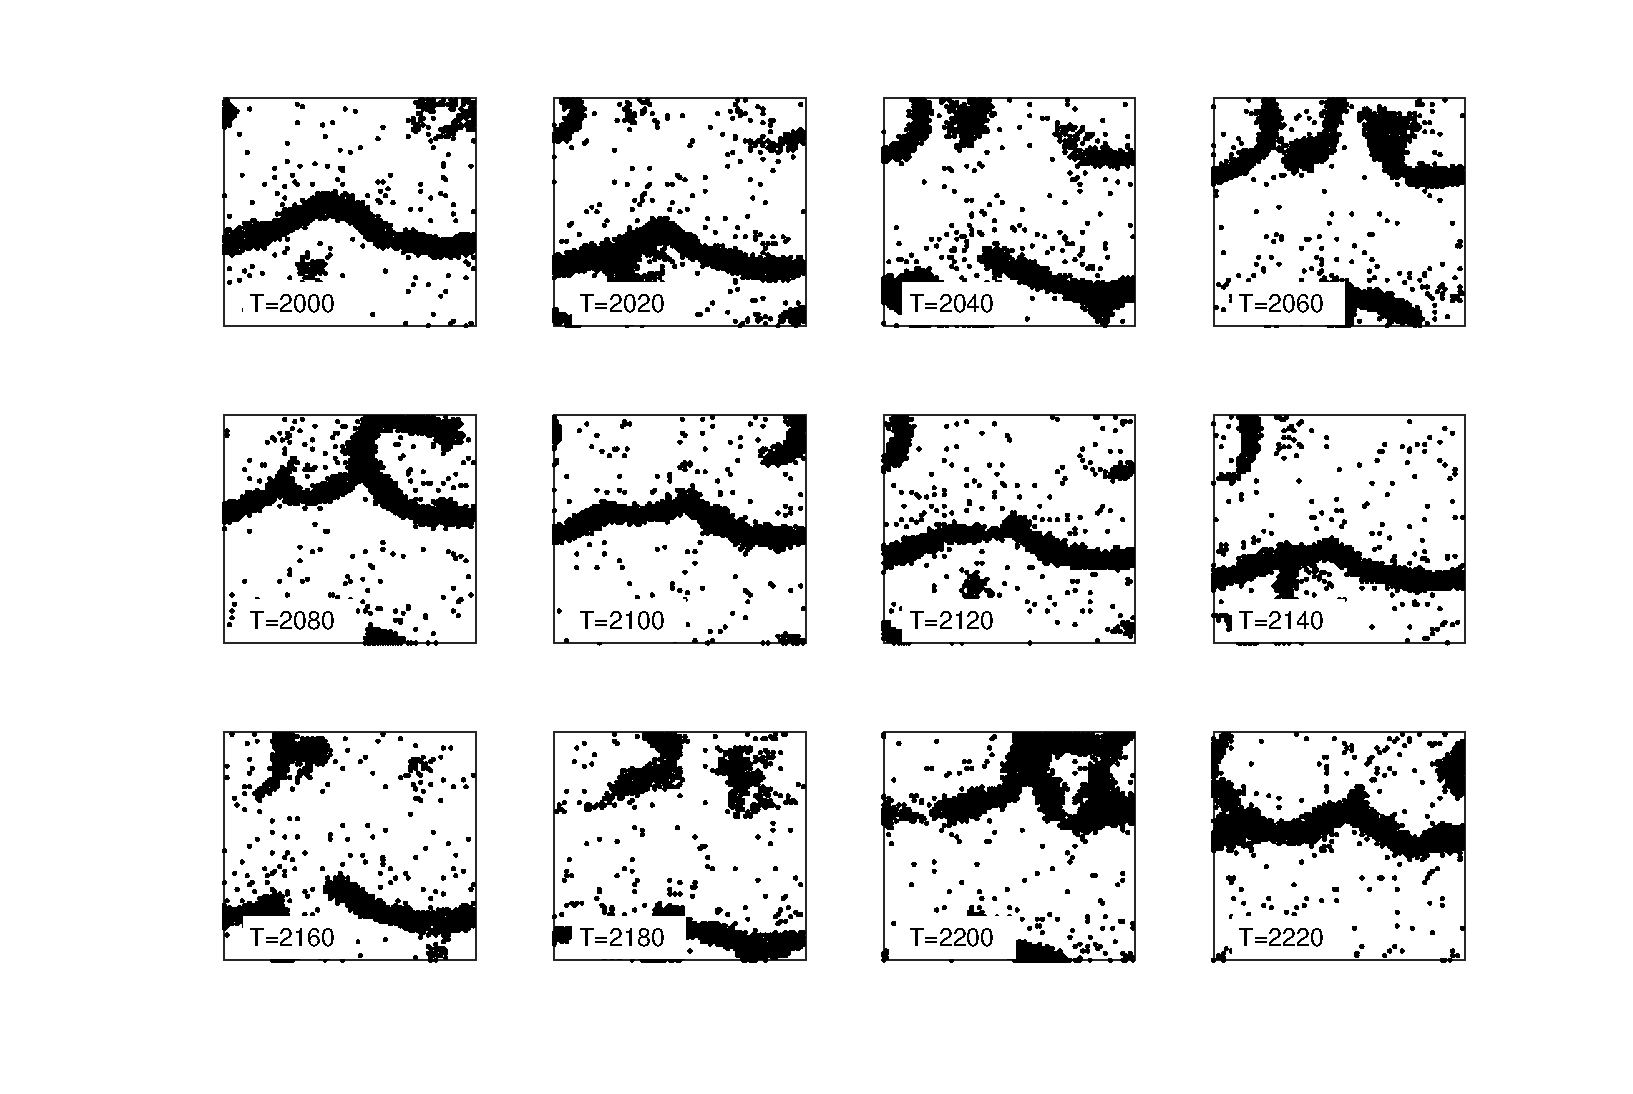
\includegraphics[width=\textwidth]{fig/2DWaveRasters_PlaneWave}
\end{figure}
\FloatBarrier

When the wave speed increases we observe attractor states, where waves spawned from a small number of locations come to dominate the firing activity.
In figure \ref{fig:2DWaveRasters_attractor} we see that the waves come to dominate the firing activity.
\begin{figure}[!htb]
 \caption{ Raster plots from our quasi 2-D system showing an attractor forming near X=70,Y=75.}
 \label{fig:2DWaveRasters_attractor}
 \centering
   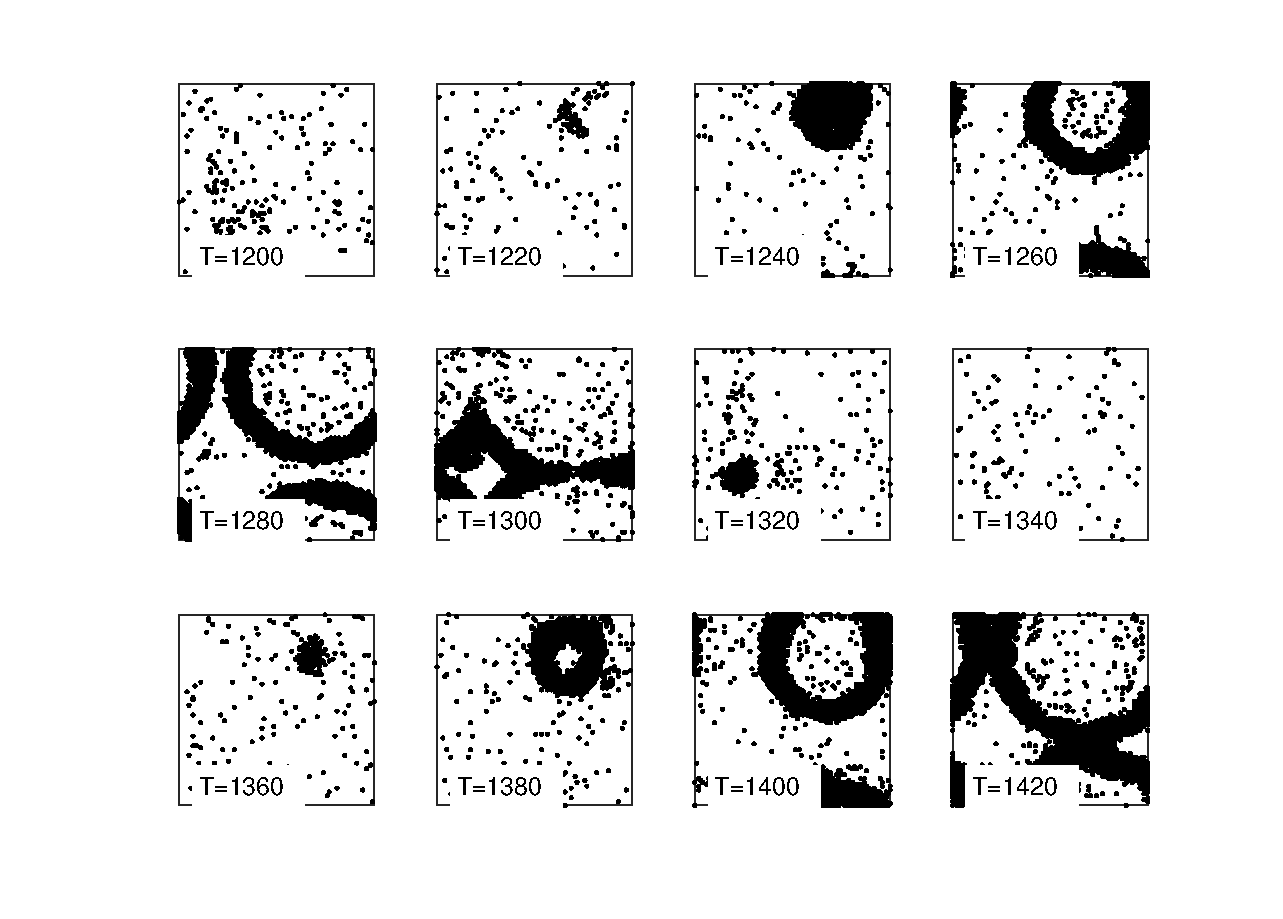
\includegraphics[width=\textwidth]{fig/2DWaveRasters_Attractor_kappa0p1_seed35}
\end{figure}

We suspect that these winner-take-all waves may be spawned by low-threshold spiking inhibitory neurons as seen in our minicolumns (section \ref{sub:wave_initiation}).
To test this hypothesis we plot calculate the density of inhibitory neurons across the sheet using MATlAB's 'ksdensity' function.
\begin{figure}[!htb]
 \caption{ Density plot of inhibitory neurons in the sheet. The color scale covers the top 10\% of the density.
           The area with the highest density of inhibitory neurons includes the location from which the attractor waves are spawned. }
 \label{fig:2DAttractor_InhibDensity}
 \centering
   \includegraphics[width=\textwidth]{fig/2DAttractor_seed35_InhibitoryDensity}
\end{figure}

\FloatBarrier

We do not observe spiral waves in our simulations with the model parameters set at $\Sigma$.
With the higher connectivity observed in the sheet (figure \ref{fig:connection_delay_distrbution_2D}) we see circular waves emanating from a point.
Although these waves can combine to form a plane wave structure (figure \ref{fig:2D_plane_wave}), we have not observed spiral wave patterns.
Given that the sheet has higher connectivity than the minicolumn, we reduce the connection strength K from $K=10$ to $K=6$.
The waves at the lower connection strength are thinner and sparser.
We now observe the formation of spiral wave pattern in figure \ref{fig:2DWaveRasters_Spiral}.
\begin{figure}[!htb]
 \caption{ Raster plots showing spiral wave behavior, especially in the center left. The sheet is 200x200x2, $K=6$, $\kappa=0.4$ }
 \label{fig:2DWaveRasters_Spiral}
 \centering
   \includegraphics[width=\textwidth]{fig/2DWaveRasters_SpiralWave}
\end{figure}
\FloatBarrier

In \citet{keane2015} traveling waves in 2-D sheets were proposed to explain simultaneous spike timing irregularity with fluctuations in the average firing rate of the ensemble. 
Despite the complex spatiotemporal patterns the overall mean voltage shows a small, steady oscillation.
\begin{figure}[!htb]
 \caption{ After initial fluctuations settle out, the system mean voltage settles into small oscillations.}
 \label{fig:2D_mean_voltage}
 \centering
   \includegraphics[width=\textwidth]{fig/MeanVoltage_PBC}
\end{figure}

\FloatBarrier

\section{Forests of minicolumns}
Our forest of minicolumns is an ensemble of 400 or 600 minicolumns arranged in a 20x20 or 30x30 pattern.
Each minicolumn is 2x2x10.
A small example foresst is shown in Figure \ref{fig:forest_structure}.
\begin{figure}[!htb]
 \caption{ Example forest of 16 minicolumns arranged in a 4x4 grid, with $1\lambda$ spacing between the closest neurons of any two minicolumns. 
              Each minicolumn has dimensions X=2, Y=2, Z=5, $\lambda$=2.5, and C=0.5. 
          a)  Sheet showing connections between neurons as lines colored using a color scale that indicates the connection length. 
          b)  Connection matrix. E-E connections are green, E-I are black and both I-E and I-I  are red. }
 \label{fig:forest_structure}
 \subfloat[][]{\includegraphics[width=0.75\textwidth]{fig/Forest_Structure_A}}
 \subfloat[][]{\includegraphics[width=0.75\textwidth]{fig/Forest_Structure_B}}
\end{figure}
\FloatBarrier

We wish to compare the overall 
The distribution of post-synaptic connections and delay times are shown in Figure \ref{fig:connection_delay_distrbution_forest} for an example minicolumn.
\begin{figure}[!htb]
 \caption{Distribution of (a) number of post-synaptic connections per neuron and (b) delay time. Data was taken from a 20x20 forest of 400 minicolumns, each minicolumn 2x2x10, $\lambda=2.5$, $\kappa=1$.  } 
     \subfloat[][]{\includegraphics[width=0.6\textwidth]{fig/ConnectionNumberDistributionForest} }
     \subfloat[][]{\includegraphics[width=0.6\textwidth]{fig/DelayDistributionForest} }
 \label{fig:connection_delay_distrbution_forest}
\end{figure}
 \FloatBarrier

We stimulate the forest with a uniform background stimulus. 
With $M=5$ there are many competing waves resulting in small-scale waves with many collisions.
We decrease M to 2 and increase K from 10 to 14.
We then observe traveling wave patterns in the forest.
\begin{figure}[!htb]
 \caption{ Raster plots from a forest of minicolumns with uniform background stimulus.}
   \includegraphics[width=\textwidth]{fig/ForestWaveRaster_Background_K14_M2}
   \label{fig:ForestBackground}
\end{figure}

We perform individual wave trials as in section \ref{sub:propagation_speed}.
In this case stimulate the minicolumn at X={0,1}. Y={0,1}.
We stimulate the first two layers Z={1,2}.
We observe a single wave traversing the forest in Figure \ref{fig:2_5D_Wave}.
\begin{figure}[!htb]
 \caption{ Raster plots from a forest of minicolumns looking down on the X/Y plane. 
           The 2x2 minicolumn in the lower left corner was stimulated at time $t=10\ ms$.}
   \includegraphics[width=\textwidth]{fig/Rasters_2_5D_Wave}
   \label{fig:2_5D_Wave}
\end{figure}


\FloatBarrier


\endinput
%%
%% End of file `example-1.tex'.

%%
%% This is file `example-1.tex',
%% generated with the docstrip utility.
%%
%% The original source files were:
%%
%% drexel-thesis.dtx  (with options: `example-part')
%% 
%% This is a generated file.
%% 
%% Copyright (C) 2010 W. Trevor King
%% 
%% This file may be distributed and/or modified under the conditions of
%% the LaTeX Project Public License, either version 1.3 of this license
%% or (at your option) any later version.  The latest version of this
%% license is in:
%% 
%%    http://www.latex-project.org/lppl.txt
%% 
%% and version 1.3 or later is part of all distributions of LaTeX version
%% 2003/06/01 or later.
%% 

\chapter{Neuron population activity encoding and transport via traveling waves in neuronal systems }

Individual neurons in the brain are tuned to fire upon specific events such as visual stimuli of a particular type \citep{Hubel1962} .
However, even neurons that are tuned to a specific stimulus show variability in their firing rate and timing when the same stimulus is repeatedly applied \citep{Georgopoulos1982}\citep{Newsome1989}.
This indicates that information in the brain is represented by the firing dynamics of populations of many neurons.
This population coding may take the form of variations in the average firing rate of the neurons in the population (rate coding) or variations in the synchronization between spikes (temporal coding).
The temporal and rate coding may also have a functional relation, i.e. through Hebbian learning \citep{Basawaraj2019}.
Various methods of decoding the information in these population dynamics have been studied \citep{Deneve1999}\citep{Xu2019}, and population dynamics are incorporated into modern theories of neural computation \citep{Pitkow2017}\citep{Nadeau2020}.

Traveling waves of neuronal activation have been observed in the cortex as reviewed in \citet{Muller2018}.
Various functional roles have been proposed for these traveling waves including spatiotemporal processing in the visual cortex \citep{wu2008}\citep{Muller2014}, place field coordination in the hippocampus \citep{lubernov2009}, and memory consolidation during sleep \citep{Dickey2021}.
Traveling waves have been shown to carry information in the  motor cortex \citep{Rubino2006} and visual cortex \citep{Besserve2015}.
These waves can provide synchronous activations of a population to serve functions such as gating perception of low-contrast images \citep{Davis2020}.
In addition to extensive observations in vivo, traveling waves have also been observed in neuronal network simulations at the mesoscopic level in simple one-dimensional systems \citep{Wilson1973}\citep{Golomb1999} and two-dimensional sheets \citep{keane2015}.
Traveling waves have also been studied in large-scale simulations of the entire brain \citep{Roberts2019}.

Previous studies have used one-dimensional structures largely for their computational or analytic simplicity. 
Consideration of a quasi one-dimensional system may seem as an unnecessary complication, but there is no a priori reason that quasi one-dimensional traveling waves may not be found in vivo.
Of interest, there are regions of the brain where there are what seem to be quasi one-dimensional structures \citep{mountcastle1997}\citep{Cruz2009} typically called micro- or minicolumns. 
These minicolumns are aligned perpendicular to the pia and can be hundreds of microns long.  
Although their relevance to cognition and function is still being debated \citep{horton2005}\citep{buxhoeveden2002}, it is possible that they can sustain traveling waves.

Here we consider how quasi one-dimensional neuronal structures could encode and transmit population activity via traveling waves.
We perform computational experiments using a quasi one-dimensional model we call a Small Columnar Ensemble (SCE), first reported in , with a network of Izhikevich neurons \citep{izhikevich2003} using the same local connectivity model as \citep{maass2002}.
We have previously shown that this model supports stimulus-evoked traveling waves across a variety of model parameters.
We now demonstrate that input from a population of neurons, simulated as Poisson spike trains, can evoke traveling waves in our quasi one-dimensional system.
The number of waves per second that span the SCE, which we term the wave arrival rate, increases as the average firing rate of the input pool of neurons is increased.
The plot of wave arrival rate versus input population firing rate resembles the activation functions of either a single neuron or a population of neurons.
This leads us to consider the SCE to have a nonlinear activation function in terms of input population rate, and to consider the SCE as encoding the input population firing rate into the wave arrival rate.

Just as a single neuron may be susceptible to noise or damage, a single SCE may also be an unreliable means of encoding and transmitting population rate information.
We therefore look at morphologies of multiple redundant SCE to enable reliable encoding and transport.
We find that simply increasing the cross-section of the SCE ...

We performed a series of computational experiments to determine how our SCE can encode and transmit population activity.
We first verified that our population of Poisson neurons can invoke traveling waves in a single SCE.
The wave rate in the single SCE was found to be proportional to the instantaneous firing rate of the population of Poisson neurons.
The relationship between population activity and wave rate resembled the activation functions of both single neurons and populations of neurons, so we termed this relationship the activation function of the SCE.
The activation function of the SCE showed significant variation across trials with randomly generated stimuli, indicating that the population rate encoding was not reliable.
We then created SCE with larger cross-section (X and Y extents) with varying topologies and observed that an ensemble of multiple SCE with loose coupling between them reduces the variation in the activation function.

\subsection{Traveling waves are evoked by population activity}
Our first configuration is an SCE with dimensions $2x2x40$ (X/Y/Z).
The SCE parameters are $C=0.5$, $\lambda=2.5$, $\kappa=0.1$, $K^{SCE}=24$ and $K^{stim}=6$.
The other parameters are fixed for all experiments as described in Methods.

We stimulated the SCE using several instantaneous firing rates for the input population.
Traveling waves are evoked in the SCE for higher firing rates (Figure \ref{fig:sce_raster}).

\begin{figure}[!htb]
 \centering
 \includegraphics[width=\textwidth]{fig/SCE_2x2_FRE_rasters}
 \caption{Poisson spike trains in the input population (bottom) evoke traveling waves in the SCE (top). Raster plots are shown for firing rates of 1 spike/second (left), 5 spikes/second (middle) and 21 spikes/second (right).  }
 \label{fig:sce_raster}
\end{figure}

\FloatBarrier

\subsection{The SCE possesses an activation function}
We stimulated the SCE with instantaneous firing rates from 1 to 21 spikes/second, with 100 random inputs created for each firing rate.
The resulting waves rates are shown in Figure \ref{fig:sce_activation_function}.
The mean wave rate showed a clear trend that is similar to a logarithmic curve. 
It also resembled the population activation rate shown in \citet{Trappenberg2010} Eq. 3.43 for the population response to slowly varying inputs:
\begin{align}
 g(x) &= \frac{1}{t^{ref}-\tau \log{(1-\frac{1}{\tau x})}}
\end{align}
where $t^{ref}$ is an absolute refractory period and $\tau$ is the charateristic response time.
We therefore consider our SCE to have an nonlinear activation function when stimulated by a  population of neurons.
This demonstrated that the SCE can be said to encode the population rate into the wave rate in a analogous manner to which single neurons and populations of neurons encode their stimulus strength into their firing rate.

\begin{figure}[!htb]
 \centering
 \includegraphics[width=\textwidth]{fig/SCE_2x2_FRE}
 \caption{The SCE encodes the input population firing rate into the wave arrival rate. }
 \label{fig:sce_activation_function}
\end{figure}

Although the mean wave rates showed a clear trend, the trial-to-trial wave rates were highly variable. 
This indicates that our SCE would not reliably encode population rate into wave rate.

\FloatBarrier

\subsection{Adding redundant columns to the SCE can reduce variability in the activation function}
Like our SCE, individual neurons also have variable firing responses to identical stimuli.
This variability is one of the key motivations for the population activity theories of information encoding in the cortex.
We next followed a similar approach and investigated the activation function of a population of multiple redundant SCE.
Several populations of SCE were generated with different distance (and therefore connectivity), between the individual SCE.
We found that a population of four SCE, with the individual SCE separated by $2\lambda$, produced a much smoother activation function.
A population of four widely separated SCE with no connectivity between them was still highly variable.


\begin{figure}[!htb]
 \centering
 \includegraphics[width=\textwidth]{fig/OneLambdaFourLambda}
 \caption{Activation functions of a population of 4 SCEs. 
	    A: When the SCE are spaced $2\lambda$ apart the activation function shows greatly reduced variability. 
	    B: When the SCE are widely spaced with no connectivity between the SCE there is still substantial variability in the activation function.}
 \label{fig:sce_4x4_coupled_activation_function}
\end{figure}

\FloatBarrier


\endinput
%%
%% End of file `example-1.tex'.

%%
%% This is file `example-1.tex',
%% generated with the docstrip utility.
%%
%% The original source files were:
%%
%% drexel-thesis.dtx  (with options: `example-part')
%% 
%% This is a generated file.
%% 
%% Copyright (C) 2010 W. Trevor King
%% 
%% This file may be distributed and/or modified under the conditions of
%% the LaTeX Project Public License, either version 1.3 of this license
%% or (at your option) any later version.  The latest version of this
%% license is in:
%% 
%%    http://www.latex-project.org/lppl.txt
%% 
%% and version 1.3 or later is part of all distributions of LaTeX version
%% 2003/06/01 or later.
%% 

\chapter{Conclusion}

\section{Quasi 1-D results}
Here we have demonstrated that a biologically influenced model of a small quasi one-dimensional columnar ensemble  can support traveling waves. 
Our model considers a wide variety of neuronal types using local connectivity and distance-dependent time delays.
Because of the substantial randomness in neuronal types and connections between neurons, we did not observe traveling waves in the purely one-dimensional ($X=1,Y=1$) version of our model, 
in contrast to previous work that considered traveling waves in homogeneous neuronal populations in strictly one-dimensional systems. 

In our model various parameters determine traveling wave formation and propagation including the connectivity, connection strength and excitatory/inhibitory balance.
Columns with local connectivity support traveling waves, consistent with other simulations and experimental studies of cortical traveling waves \citep{Kopell1986}\citep{ermentrout2001}\citep{Golomb1999} .
The speed of these waves are influenced by connectivity, with a logarithmic dependence on connection strength that is consistent with previous work \citep{Golomb1996}\citep{Golomb1999}.

We have also shown that  a fully-connected SCE exhibits traveling waves if the action potential propagation time depends on the inter-neuron distance. 
From the dynamics point of view, we have shown that the action potential propagation delays affect propagation speed (Figure \ref{fig:delay_speed}) but is not a determinant on whether a wave can exist 
(Figure \ref{fig:wave_parameters}d).
We have also shown that  the connectivity and connection strengths influence the wave propagation speed (Figures \ref{fig:delay_k} and \ref{fig:delay_topology}) 
through the neuron dynamics (Figure \ref{fig:delay_neurondynamics}) .
From the point of view of neuronal types  we have determined that preferential sites for wave initiation are due to the presence of inhibitory neurons with low spiking thresholds.

Previous research into traveling waves in neuronal networks has identified parameter regions of neural-field models for which traveling waves exist \citep{Wilson1973}\citep{Ermentrout1979}. 
In these models critical values of model parameters are usually revealed by a linear stability analysis.
Our exploration of model parameters (Figure \ref{fig:wave_parameters}) instead shows a gradual transition region in which waves emerge and dominate the firing activity.
In \citep{Senk2020} the authors derive critical parameters using linear stability analysis of a neural field and find the critical parameter values, then map those parameters
to a network of leaky integrate-and-fire neurons.
Although the stability analysis shows sharply defined regions (their Figure 3 and 4), their spiking neuron simulation results show a gradual transition between regions (their Figure 7) similar to our work.

We have investigated the effect of incrementally increasing the dimensionality of our SCE on the speed and existence of traveling waves by considering a larger base (width described by X and Y) 
but still preserving its quasi one-dimensional character (ratio of Z to X or Y from 50 to greater than 7).
Our results show that the speed of the traveling waves initiated at the bottom of the SCE increased as a function of width (Figure \ref{fig:delay_topology}).
This can be understood by noting that we use open boundary conditions that when considering a larger width will inevitably increase the average number of connections per neuron in the SCE.
This means that neurons on average will receive a higher input current that, by its similarity to the mechanisms behind Figure \ref{fig:delay_k}, will cause a higher speed. 
We further show that the increased number of connections per neuron is the sole mechanism behind this effect by obtaining a constant speed when keeping constant the average number of connections
(Figure \ref{fig:delay_topology_avgconn}).
By using the same system with a constant number of connections per neuron, but now using a background stimulation to all neurons, we show that the value of the connection strength beyond which traveling waves (or synchronous firing) exist is very similar to that shown in Figure \ref{fig:wave_parameters}a, independent of width of SCE (SI Figure 5).
Moreover, the graphs of raster plots as a function of width seem to indicate that there is a value for the width at which excitations change from traveling waves to synchronous firing (SI Figure 5).
Future work will consider whether this change represents a phase transition between traveling waves and synchronous firing, a transition that is not uncommon to find in other systems but controlled by other intrinsic coupling parameters \citep{ermentrout2001}\citep{Senk2020}.

Other research \citep{keane2015} has shown that complex spatial patterns emerge from two-dimensional networks of leaky-integrate-and-fire neurons when the excitation and inhibition are balanced.
In that work, when excitation dominates then only plane waves were observed instead of complex patterns.
Similarly, in one dimension we have found that traveling waves dominate the firing activity when the $P_{exc}$ grows close to $1$ (Figure \ref{fig:wave_parameters}).
Both studies show that traveling waves can become the dominant spatial pattern in excitatory networks.

We have found that low-threshold-spiking inhibitory neurons can determine the origin point of traveling waves when using a uniform background stimulus (Figure \ref{fig:lts_inhibit}).
Parameter variations in the Izhikevich model \citep{izhikevich2003} create low-threshold spiking found in some inhibitory neurons \citep{gibson2009}\citep{hayut2011}, leading to post-inhibitory rebound spiking in the connected excitatory neurons \citep{ascoli2010}.
Our result is fundamentally different than previous studies of oscillatory behavior in populations of coupled excitatory and inhibitory neurons \citep{Golomb1996}\citep{Golomb1999} as that work considered homogeneous populations with isotropic connectivity.
\citet{Sessolo2015} found that stimulating inhibitory neurons in vitro could eithertrigger or inhibit epiletiform activity depending on the location of the stimulus.

Our result implies that, when no stimulus is applied, a biological neuronal network might have an equilibrium dynamics governed by traveling waves initiated by low-threshold-spiking inhibitory neurons.
An applied stimulus could then disturb the network from this dynamic equilibrium state.
Our results show  that any network with sufficiently strong connectivity and delayed action potential propagation can exhibit traveling wave structure (Figure \ref{fig:delay_waves}).
Since biological action potentials always travel with some delay, this indicates that traveling waves could be observed in the brain regardless of the inter-neuron connectivity.
The numerical results presented here could be further refined to predict biological traveling wave speed for different neuron and network parameters.
This could help distinguish between the different classes of traveling waves presented in \citet{ermentrout2001}.

Traveling waves in one-dimensional networks have not been observed in the brain. 
Part of the reason might be that such an observation requires precise experiments that probe structures such as minicolumns in the cortex. 
These are not easy, as other properties of minicolumns are still elusive. 
However, our work shows that in biological quasi one-dimensional systems  traveling waves are not only possible, but that because of the wide range of values in their allowed parameter space, their existence should be expected.

\section{Quasi-2D results}
We have demonstrated traveling waves in quasi two-dimensional sheets with substantial spatial variation in the neurons and synapses.
Previous two-dimensional simulations using neural field models or leaky integrate-and-fire neurons addressed systems of identical neurons and isotropic connections.
In our model a purely two-dimensional system did not exhibit traveling waves, although it did exhibit spatial and temporal correlations in the neural activity.

We have shown that our model can exhibit the circular spreading waves, plane waves and spiral waves that are observed in the cortex.
The spiral waves are most prevalent at lower connection strengths.
We have shown that a single spreading wave can fracture into a spiral wave due to the variation in the underlying neural system.

Our quasi-2D sheets exhibit repeating spatio-temporal wave patterns.
These patterns are fairly stable over time and we consider them as attractor states of the system.
A given sheet can exhibit multiple attractor states, as applying different random background stimulus to the same sheet results in different wave patterns.

Previous work \citep{keane2015} proposed traveling waves as an explanation for the seeming contradictions between the irregular spiking behavior of individual neurons 
and the correlation between the firing of nearby neurons.
We reproduce these results, showing substantial variance in the inter-spike intervals as well as higher correlation between the firing rates of nearby neurons.
We confirm that the neurons mostly fire when a traveling wave passes, but any individual neuron may not fire at all or fire multiple times when a particular wave passes.
We also find that for the special case of sparse connectivity our systems can exhibit extremely regular inter-spike intervals if each neuron fires only once when a wave passes.

We have also demonstrated traveling waves in a forest of minicolumns that represents the laminar and minicolumnar organization of the cortex.
The forest organization creates anisotropy between the vertical connectivity (down the minicolumn) and the lateral connectivity between minicolumns.
Transverse traveling waves are supported in the forest even when the lateral connectivity is lower than would normally permit wave propagation.
We observe both spreading and spiral waves structures depending on the connection strength.
The transverse wave speed is slower than the vertical wave speed within the minicolumns.


\section{Information transport}
We have proposed a mechanism for the encoding and transport of the information contained in the activity of a population of neurons via traveling waves of neuronal activation.
We demonstrated that our minicolumn structure can encode the population firing rate into the minicolumn wave rate.
The minicolumn wave rate depends asymptotically on the firing rate of the input population in a manner that resembles the activation functions of both single neurons and neural populations. 
Although the single minicolumn encoding was noisy, we demonstrated that a forest of loosely coupled  minicolumns could more reliably encode and transmit the population rate information.

\section{Future work}
The present work has established fundamental methods and results for exploring traveling waves in simulations of neuronal systems.
There are a number of areas for further research based on the results shown so far.

The present models do not include time-varying connection strengths or any model of synaptic plasticity.
A common form of spike-timing-dependent plasticity enhances a synaptic connection between two neurons when the presynaptic neuron fires shortly before the postsynaptic neuron fires.
Since traveling waves naturally impose a spatial sequence to the neuron firing activity it is reasonable to expect that synaptic plasticity could enhance traveling waves.
Traveling waves could even be an emergent behavior due to the long-term potentiation of synaptic pathways in a given direction.

We have observed that a given quasi two-dimensional system can settle into different attractor states.
It is possible that an external stimulus could cause a system in one attractor state to switch to a different attractor state.
Such stimuli-induced switching between stable states would be an interesting phenomenon with a number of possible functional roles.

The present work does not include any representation of the damage that may occur to neurons and synapses due to trauma, disease or aging.
Previous work \citep{cruz2000} has shown a loss of minicolumnar structure in the cortex of sufferers of Alzheimer's disease.
Our methods could be extended to examine how such changes to cortical organization could disrupt the formation and structure of traveling waves

We have shown that a small forest of minicolumns can both encode and transport information.
Such a structure might also perform a filtering function by e.g. selectively transmitting certain stimulus frequencies.
The coupling between adjacent minicolumns may also provide a mechanism for spatial filtering if different stimuli are applied to different minicolumns. 
Such an experiment is suggested by the observed columnar structure of the visual cortex in which neurons in the same column are tuned to the same stimulus.

Our minicolumn structure was inspired by the neuronal structure described in the seminal paper on Liquid State Machines \citep{maass2002}.
The structures presented here could be used as the 'liquid' or 'reservoir' in that paradigm of machine learning.
The waves observed in the quasi-two dimensional systems are reminiscent of the ripples in a pool of water from a falling stone, 
the analogy that inspired the term Liquid State Machine.

Interaction between temporal oscillations at different frequencies, termed cross-frequency coupling \citep{Hyafil2015}, has been observed in mammalian brain.
One widely studied example is the relationship between theta oscillations ($4-8~Hz$) and gamma oscillations ($>30~Hz$), 
which have been proposed as a means to represent multiple items in an ordered way \citep{Lisman2013}. 
The present work has produced traveling waves with repetition rates in the theta range.
This work could be extended with models that include higher-frequency oscillations to study the mechanisms and computational roles of cross-frequency coupling.

\endinput
%%
%% End of file `example-1.tex'.

\end{thesis}

\bibliography{thesis}

%\appendix
%\include{}

%\begin{vita}

%\end{vita}

\end{document}
\endinput
%%
%% End of file `example.tex'.
